\documentclass[a4paper,12pt,twoside]{article}

%===========PACOTES
\usepackage[body={173mm,235mm}]{geometry}
%\usepackage[portuguese]{babel}
\usepackage{a1}
\usepackage[english]{babel}
\usepackage[latin1]{inputenc} %permite o uso de acentos
%\usepackage[dvips]{color}
\usepackage{amsfonts,amssymb}
%\usepackage{epsfig}
\usepackage{amsmath}
\usepackage{graphicx}
\usepackage{float}

% makeidx
\usepackage{makeidx}
% make index
\makeindex
%\usepackage[pdftex]{graphicx}


\def\mapright#1#2#3{\smash{\mathop{\hbox to
#3{\rightarrowfill}}\limits^{#1}_{#2}}}

\def\mapleft#1#2#3{\smash{\mathop{\hbox to
#3{\leftarrowfill}}\limits^{#1}_{#2}}}

\def\mapright#1#2{\smash{\mathop{\hbox to 0.90cm{\rightarrowfill}}\limits^{#1}_{#2}}}
\def\mapleft#1#2{\smash{\mathop{\hbox to 0.90cm{\leftarrowfill}}\limits^{#1}_{#2}}}

\def\mapleftright#1#2{\smash{\mathop{\hbox to 0.80cm{\leftarrowfill \rightarrowfill}}\limits^{#1}_{#2}}}
\def\ext{\times \! \vrule depth0pt height5pt width0.35pt}

\def\H{\mathcal H}
\def\D{\mathcal D}
\def\B{\mathcal B}
\def\C{\mathbb C}
\def\R{\mathbb R}
\def\S{\mathbb S}			
\def\U{\mathcal U}
\def\Z{\mathbb Z}

\title{PL-embedding the dual of two Jordan curves \\ 
into $\mathbb{S}^ 3$ by an $O(n^ 2)$-algorithm
\footnote{2010 Mathematics Subject Classification: 
57M25 and 57Q15 (primary), 57M27 and 57M15 (secondary)}} 
\author{S�stenes Lins and Ricardo Machado}

\date{\today}


\begin{document}

\maketitle
%\input{global}
%

\section{Introduction}
A {\em $J^ 2$-gem} is a 4-regular, 4-edge-colored planar graph $G$ obtained from the
intersection pattern of two Jordan curves $X$ and $Y$ with $2n$ transversal
crossings.
These crossings define consecutive segments of $X$ alternatively 
inside $Y$ and outside $Y$. Color the first type 2 and the second type 3.
The crossings also define consecutive segments of $Y$ alternatively 
inside $X$ and outside $X$. Color the first type 0 and the second type 1.
This defines a 4-regular 4-edge-colored graph $G$ where the vertices are the crossings
and the edges are the colored colored segments.
Let $K$ be the 3-dimensional abstract 3-complex formed by taking a set of 
vertex colored tetrahedra in 1--1 correspondence with $V(G)$ so that each tetrahedra
has vertices of colors 0,1,2,3. For each $i$-colored edge of $G$ with ends $u$ and $v$
paste the corresponding tetrahedra $\nabla_u$ and $\nabla_v$ so as to paste the two triangular
faces that do not contain a vertex of color $i$ in such a way as to
to match vertices of the other three colors. 
We show that the topological space 
$|K|$ induced by $K$ is $\mathbb{S}^ 3$. Moreover we describe an $O(n^2)$-algorithm
to make available a PL-embedding (\cite{rourke1982introduction}) of $G^\star$ 
into $\mathbb{S}^3$. We get explicit coordinates in $\mathbb{S}^ 3$ for the 0-simplices and
the p-simplices $(p \in \{1,2,3\}$) are linear simplices in the spherical geometry.



%\input{D.sect1.gems}
% \section{Definition of Gem}
For completeness we briefly recall the basic definitions of gem theory, leading to its definition, \cite{lins1995gca}.
A {\em 4-graph} $G$ is a finite bipartite 4-regular graph whose edges are partitioned into 4 colors,
0,1,2, and 3, 
so that at each vertex there is an edge of each color, a proper edge-coloration, \cite{bondy1976gta}.
For each $i \in \{0,1,2,3\}$, let $E_i$ denote the set of $i$-colored edges of $G$.
A $\{j,k\}$-residue in a $4$-graph $G$ is a connected component of the subgraph induced by $E_j \cup E_k$.
A 2-residue is a $\{j,k\}$-residue, for some distinct colors $j$ and $k$.
A {\em gem} is a 4-graph $G$ such that for each color $i$, $G\backslash E_i$ can be embedded in the plane 
such that the boundary of each face is a 2-residue. From a gem there exists a straightforward
algorithm to obtain a closed orientable 3-manifold, in two different, dual ways. Every such a manifold is obtainable in this way.
An unecessary big gem is obtained from a triangulation $T$ for a manifold by taking the dual of the 
barycentric subdivision of $T$. Here the colors corresponds to the dimensions. Doing simplifications in the gem
completely destroys this correspondence.


\section{Wings as seeds for obtaining the dual PL-complex $\mathcal{H}_n^\star$}

This is the third of 3 closely related articles.
References for the companion papers are \cite{linsmachadoA2012} and \cite{linsmachadoB2012}.

Let $\Pi_\ell$  ($\Pi_r$) be the half plane limited by the $z$-axis 
which contains $a_1=z_0z_2/2$ $(b_1=z_1z_2/2)$.
The construction of the wings and nervures of the next section are exemplified in Figs. \ref{fig:winglist01} to \ref{fig:winglist11}.

\subsection{Wings: reformulating a difficult 3D-problem 
into an easy planar one}\label{subsec:wings}

At some point in our research it became evident that what was needed to obtain the PL-complex $\mathcal{H}_n^\star$ 
was a proper embedding into $\mathbb{R}^3$ of the set of 0-simplices $\{a_1, a_2,\ldots,a_f\} \cup \{b_1, b_2,\ldots,b_g\}$.
The other 0-simplices are obtained by bisections of segments linking previously defined points. It came as a surprise to discover
that this apparently difficult 3D problem was reformulated as a plane problem for which we had at hand an easy solution,
namely Tutte's barycentric method.

We construct a 
sequence of pairs of plane
graphs $\{\{\mathcal{W}^\ell_1,\mathcal{W}^r_1\},
\{\mathcal{W}^\ell_2,\mathcal{W}^r_2\},\ldots,
\{\mathcal{W}^\ell_n,\mathcal{W}^r_n\} \}.$ The $m$-th such pair
constitutes the {\em left} and {\em right wings} \index{wings} of the colored $2$-complex
$\mathcal{H}_m^\star$. The left wings are embedded into $\Pi_\ell$ and
the right wings are embedded into $\Pi_r$. 
We define $\mathcal{W}^\ell_1$ as the set of $2n$ straight line segments
$a_1z_3^1, a_1z_3^2, \ldots, a_1z_3^{2n} \subseteq \Pi_\ell$,
and $\mathcal{W}^\ell_1$ as the set of $2n$ straight line segments
$b_1z_3^1, b_1z_3^2, \ldots, b_1z_3^{2n}  \subseteq \Pi_r$.
The {\em outer triangular region of the left wings} is the plane region
spanned by $a_1, z_3^1,z_3^{2n}$. The {\em outer triangular region of 
the right wings} is the plane region spanned by
$b_1, z_3^1, z_3^{2n}$. 
The passage from $\{\mathcal{W}^\ell_{m-1},\mathcal{W}^r_{m-1}\}$
to $\{\mathcal{W}^\ell_m,\mathcal{W}^r_m\}$ in the $(m-1)$-th $bp$-move,
which we call a {\em $wbp$-move}, corresponds
in $(\mathcal{H}_{m-1}, \mathcal{H}_{m})$ to either a 
0-flip that subdivides a 13-gon into two (case
where the tail of the balloon is of color 0)
or else to a 1-flip that subdivides a 03-gon into two (case
where the tail of the balloon's is of color 1).  
At this point, we need to define a tree called the \index{nervure of a wing} {\em nervure of a wing}.
This is done inductively.
The first ones, $\mathcal{W}^\ell_1$ and $\mathcal{W}^r_1$ have, respectively 
the degenerated trees formed by single points $a_1$ and $b_1$ as their nervures.
In the unique wing that changes with the $bp$-move, a vertex $x_\ell$ corresponding
to either a 13-gon or else to a 03-gon (in a way to be made clear in the poof of
Lemma \ref{lem:internalpointsbigons}).
The intersection of the balloon's head and 
its tail in $\mathcal{H}^\star_m$ is a PL1-face formed by two
simplices meeting at a point $a_p$ (if the tail of the balloon is of color 1)
or $b_q$, if it is of color 0. 
Along the process we define the following auxiliary functions, with arguments
%$1 \le m \le n-1$ or
 $1 \le m \le n-1$:  
$c(m),u(m),v(m),r(m),s(m),
\ell_a(m), \ell_b(m), t_a(m), t_b(m).$
The color
of the $m$-th balloon's tail is denoted by $c(m) \in \{0,1\}$.
Let $u(m), v(m)$ be the odd and even indices of the $m$-th 
balloon's head $\nabla_{u(m)} \cup \nabla_{v(m)}$. 
Let $r(m), s(m)$ be the odd and even indices of the $m$-th 
balloon's tail given by the PL2$_{c(m)}$-face $\subseteq 
\nabla_{r(m)} \cap \nabla_{s(m)}$.
The positive integers $\ell_a(m)$ and $\ell_b(m)$ are the last $a$- and $b$-indices
in left $m$-th wing and right $m$-th wing, respectively.
Indices $p$ or $q$ in the $m$-th $bp$-move satisfy $p=t_a(m)$ or $q=t_b(m)$.
In the passage $\mathcal{H}_m^\star$ to $\mathcal{H}_{m+1}^\ast$ either 
vertex $a_p$ is replaced by $a_{p'},A_p,a_{p''}$, where $p'=\ell_a(m)+1$ and 
$p'' =\ell_a(m)+2$ or else
$b_q$ is replaced by $b_{q'},B_p,b_{q''}$, where $q'=\ell_b(m)+1$ and $q''=\ell_b(m)+2$,
depending on the color of the balloon's tail. In the first case, we add two new edges
$a_{p'}A_p$ and $a_{p''}A_p$ to the nervure, in the second case, we add the edges
$b_{q'}B_p$ and $b_{q''}B_q$ to the nervure. In both cases, $p''=p'+1$ or
$q''=q'+1$. In the pictures the edges of the nervure
are thicker than the ones in the respective wing.
For $1\le m\le n$, and $h\in \{\ell,r\}$, the nervure of $\mathcal{W}^h_m$, 
denoted $\mathcal{N}^h_m$, is a spanning tree of the graph 
$\mathcal{W}^h_m \cup \mathcal{N}^h_m \backslash Z$, where $Z= \{z_3^j~|~ j\in \{1, \ldots, 2n\}\}.$
See Fig. \ref{fig:controlmaps01}, Fig. \ref{fig:controlmaps01novo1},  
Fig. \ref{fig:controlmaps01novo2}
and the complete sequence of figures for the $r^{24}_5$-example, 
Figs. \ref{fig:winglist01}-\ref{fig:winglist11}. 
A vertex in the tree $\mathcal{N}^h_m$ is {\em pendant} if it has degree at most 1.



\begin{lemma}
 Let $1\le m \le n$. The set of pendant vertices of $\mathcal{N}_m^\ell$ is
in 1-1 correspondence with the set of 13-gons of $\mathcal{H}_m$. 
 The set of pendant vertices in $\mathcal{N}_m^r$ is
in 1-1 correspondence with the 03-gons of $\mathcal{H}_m$.
\label{lem:internalpointsbigons}
\end{lemma}
\begin{proof}
The intersection of the $(m-1)$-th balloon's head and tail is a 
PL1-face with two 1-simplices. Their intersection is a point in $\Pi_h$.
The PL1-face dualy corresponds to a 13-gon (resp. 03-gon) in $\mathcal{H}_{m-1}$
if $h=\ell$ ($h=r$). After the 0-flip (resp. 1-flip) that produces  $\mathcal{H}_m$
the PL1-face is splitted into two, in a conformal way with the passage 
from  $\mathcal{W}^h_{m-1} \cup \mathcal{N}^h_{m-1}$ to  
$\mathcal{W}^h_m \cup \mathcal{N}^h_m$. Given this interpretation
the Lemma is easily established by induction.
\end{proof}


%--------------------
\begin{figure}[!htb]
\begin{center}
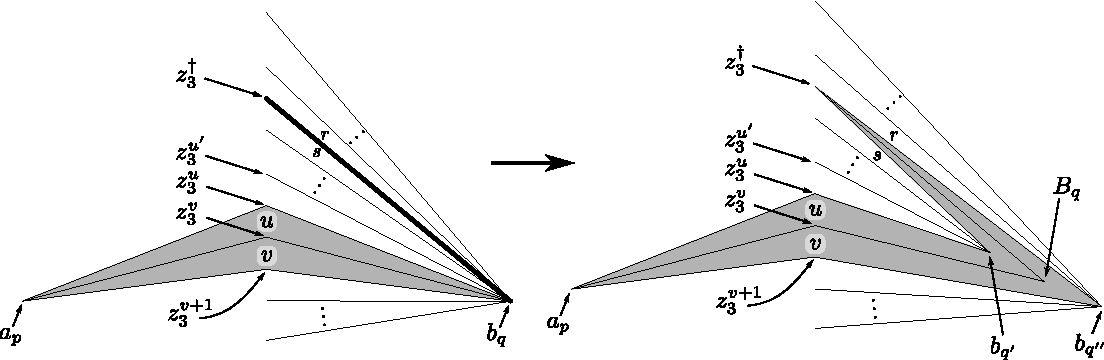
\includegraphics[width=15.4cm]{A.figs/controlmaps01.pdf}
\caption{$wbp$-move: balloon's head section is painted in gray, 
and the part of balloon's tail that is intersecting the appropriate
semi-plane is depicted as a {\em thick edge}. \index{thick edge}}
\label{fig:controlmaps01}
\end{center}
\end{figure}
%--------------------

\begin{figure}[!htb]
\begin{center}
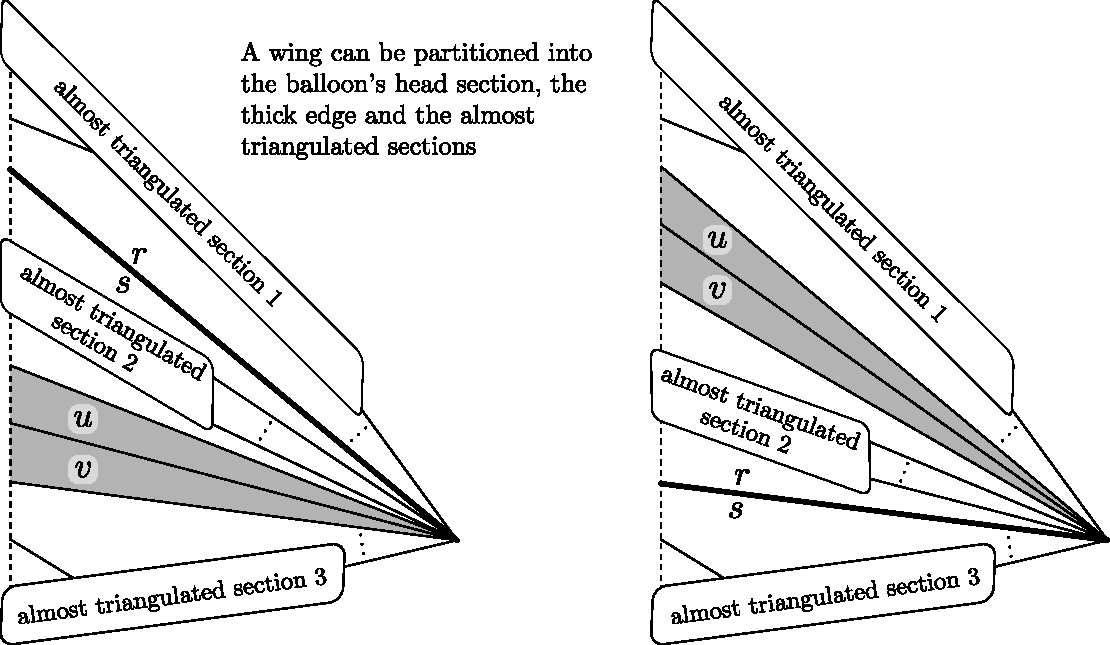
\includegraphics[width=15cm]{A.figs/controlmaps01novo1.pdf}
\caption{Given a half-wing and a balloon it can be partitioned into the 
balloon's head section, thick edge and
some {\em almost triangulated} sections.}
 %meaning that some faces are bounded by plane quadrilaterals instead of triangles.}
\label{fig:controlmaps01novo1}
\end{center}
\end{figure}

\begin{figure}[!htb] 
\begin{center}
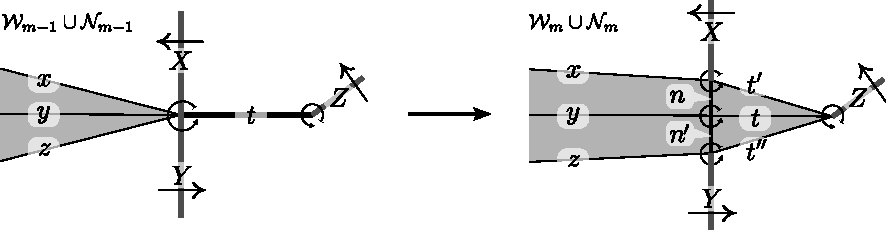
\includegraphics[width=15 cm]{A.figs/controlmaps01novo2.pdf}
\caption{The {\em star} \index{star} of a vertex of a graph embedded in a surface is the counterclockwise cyclic sequence of 
edges incident to the vertex (such an ordering is induced by the surface).
The set of stars is called a { \em rotation} \index{rotation} and has the 
characterizing property that each edge appears twice.
The general case of changing rotation when going from 
$\mathcal{W}_{\ell-1} \cup \mathcal{N}_{\ell-1}$ to
$\mathcal{W}_{\ell} \cup \mathcal{N}_{\ell}$ is depicted above. 
The rotation completely specifies the topological embedding.}
\label{fig:controlmaps01novo2}
\end{center}
\end{figure}

A graph is {\em rectilinearly embedded into $\mathbb{R}^3$} if 
the images of their edges are straight
line segments.
It is a straightforward application of Tutte's barycentric method \cite{tutte1963dg},
\cite{colin2003tutte} to obtain a rectilinear embedding of
$\mathcal{W}_n^h \cup \mathcal{N}_n^h$ which fixes the vertices in the boundary of the 
outer triangular region of $\Pi_h$, $h \in \{\ell,r\}$.
Tutte's method has an intrinsic connection with the Laplacian of graphs, see  \cite{Klarreich0412}.
We rotate $\Pi \in \{ \Pi_\ell, \Pi_r \}$
so that it becomes the $xz$-plane. After having the planar coordinates
$\Pi_h$ is rotated back to its initial position and we have the 
$\mathcal{W}_n^h \cup \mathcal{N}_n^h$ rectilinearly embedded into $\mathbb{R}^3$.
Tutte's method becomes very efficient because of Lemma \ref{lem:numberofedges}.


Tutte's method suffers of the clustering problem where vertices accumulate
in some small regions. Even though theoretically this is not 
needed, we present a heuristic of attaching weights to the edges
to improve the result. An edge with weight $k\in\mathbb{N}$ behaves
as $k$ parallel edges.
We define the weights for the edges of the wings as 1.
If the edge is in the nervure,
to calculate the weight, we use the whole wing. 
Start defining these weights as 0, so from leaves to root, 
define the weight of an edge
as the weight of the vertex incident to it and closer to 
the leaves minus 1, Fig. \ref{fig:arvorecompesos}.
In Fig. \ref{fig:controlmapsnovo6} we compare the two results,
without and with weights given by three times the weights in the nervure 
of Fig. \ref{fig:arvorecompesos}, 
for obtaining the final left wing of the $r^{24}_5$-example.


Tutte's method is applied twice: to plane graphs $\mathcal{W}_n^\ell \cup \mathcal{N}_n^\ell$ and to $\mathcal{W}_n^r \cup \mathcal{N}_n^r.$
In each application we use $O(n)$ iterations to solve a linear system in $\mathbb{C}$. This is theoretically sufficient
to achive rectilineatiry (which nevertheless can be verified). As each one of the plane graphs has less than $6n-4$ edges by Lemma \ref{lem:numberofedges}, 
the total time to obtain $\mathcal{W}_n^\ell \cup \mathcal{W}_n^r$ embedded into $\Pi_\ell \cup \Pi_r$ is $O(n^2)$.

\begin{lemma}\label{lem:numberofedges}
 The number of edges of $\mathcal{W}_n^h \cup \mathcal{N}_n^h$, $h \in \{\ell,r\}$
is at most $6n-4$.
\end{lemma}
\begin{proof}
The number of 1-simplices in the left wing and in the right wing of the 
initial complex in the sequence are both $2n$. At each one of the $n-1$ $bp$-moves
we add 4 edges either to the left or to the right wing with its nervure.
Thus each one of the final left and right wings with nervures has at most $6n-4$ edges.
\end{proof}

\begin{figure}[!htb]
\begin{center}
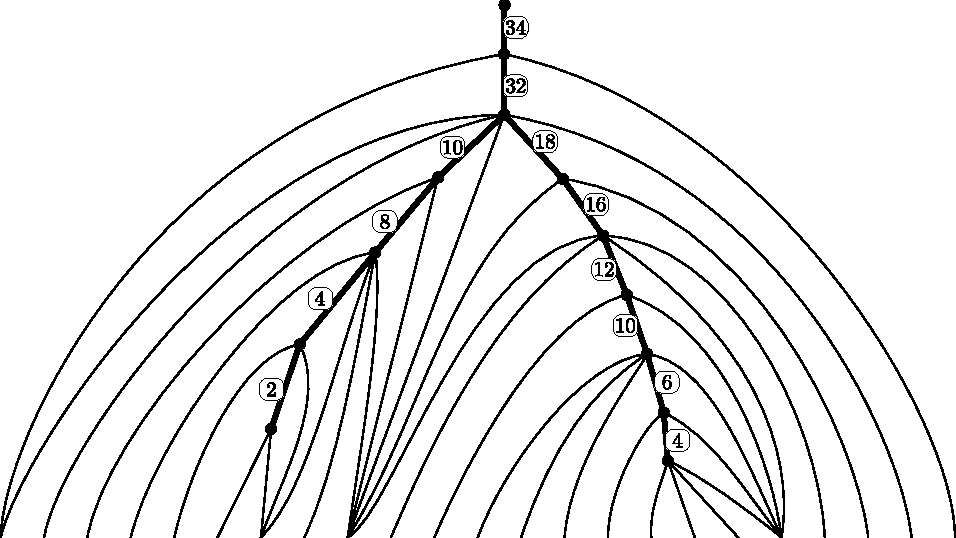
\includegraphics[width=13cm]{A.figs/arvorecompesos.pdf}
\caption{Computing the weights for Tutte's barycentric method via the wing nervure.}
\label{fig:arvorecompesos}
\end{center}
\end{figure}

\begin{figure}[!htb]
\begin{center}
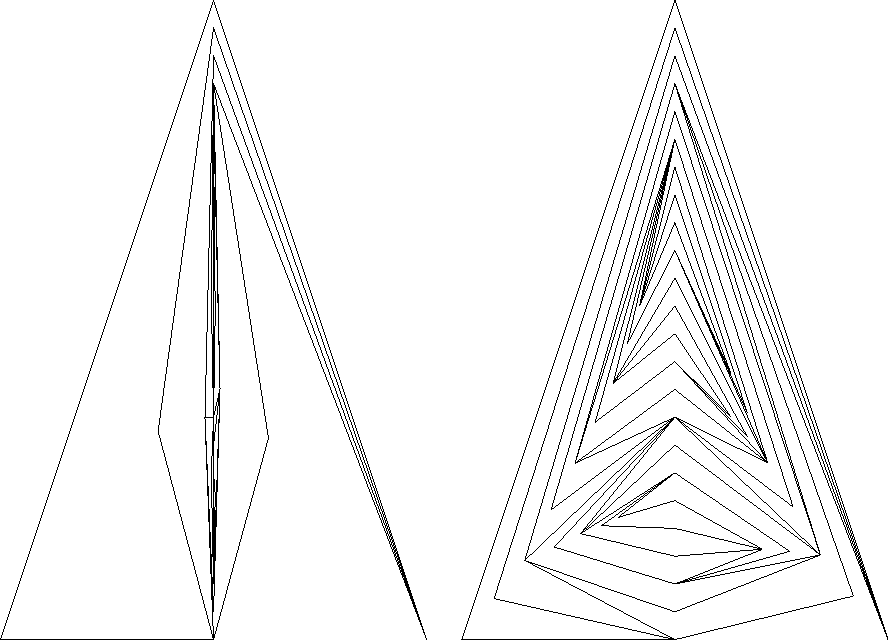
\includegraphics[width=13cm]{A.figs/controlmapsnovo6.pdf}
\caption{Tutte's embbeding without and with the weights (final pair of 
wings without nervure for the $r_5^{24}$-example).}
\label{fig:controlmapsnovo6}
\end{center}
\end{figure}
%\begin{lemma} 
%\label{theo:containement}
%$$\mathcal{U}^\star_n \subseteq (z_0 \ast W_n^\ell) 
%\cup (z_2 \ast W_n^\ell) \cup (z_1 \ast W_n^r) \cup (z_2 \ast W_n^r) 
%\bigcup_{i=1}^{2n} (z_3^i \ast z_0z_1) .$$
%\end{lemma}
%\begin{proof}
%Every 2-simplex of $\mathcal{U}^\star_m$ is contained in one of the 4+2n cones.
%\end{proof}


% 

\section{Defining the PL-embedding $\mathcal{H}_{1}^\diamond$}\label{sec:rect}


%Let $\mathcal{H}_1^\diamond=\mathcal{H}_1^\star$ be.
Let $\mathcal{L}_{i+1}^\star$ be a subset of the pillow $\mathcal{P}_{i+1}^\star$, formed by the part
that comes from the tail of the balloon after the i-th $bp$-move is applied, see Fig. \ref{fig:U3}.
%, see Fig. \ref{fig:001partenova}.
%In other words, $\mathcal{U}_n^\star=\{ v_0v_3^jv_1, v_0v_4^jv_3^j, v_4^jv_2v_3^j, v_2v_5^jv_3^j, v_5^jv_1v_3^j~|~ j\in \{ 1, \ldots, 2n \} \}$ 
%and $\mathcal{L}_n^\star=\mathcal{H}_n^\star \backslash \mathcal{U}_n^\star$, see Fig. \ref{fig:001partenova}.
%Note that $\mathcal{U}^\star_n$ denote the subcomplex  
%and
%$\mathcal{L}^\star_n$ denote the subcomplex formed by the tails 
%of the balloons or the part of the pillows that came from the tails of the balloons.

\begin{figure}[!htb]
\begin{center}
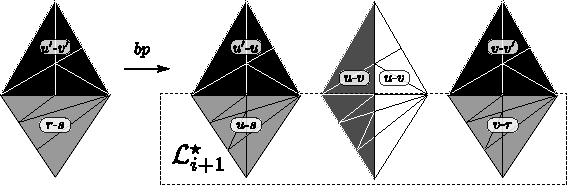
\includegraphics[width=13cm]{A.figs/U3.pdf}
\caption{The set $\mathcal{L}_{i+1}^\star$.} 
\label{fig:U3}
\end{center}
\end{figure}

%\begin{figure}[!htb]
%\begin{center}
%\includegraphics[width=14cm]{A.figs/001partenova.pdf}
%\caption{Two PL2$_3$-faces, a subset of a PL2$_0$- or PL2$_1$-face and a subset of a PL2$_2$-face (in the middle) at
% the pillow corresponding to the part that comes from the head of a balloon after all $bp$-moves be applied.}
%($\nabla_u$ and $\nabla_v$ sharing two 2-simplices in the pillow).} 
%\label{fig:001partenova}
%\end{center}
%\end{figure}


Let $\{x\} \cup Y \subseteq \mathbb{R}^N$, for $1\le N \in \mathbb{N}$. 
The \index{cone} {\em cone} \cite{rourke1982introduction} 
with vertex $x$ and base $Y$, denoted $x \ast Y \subseteq \mathbb{R}^N$,
is the union of $Y$ with all line 
segments which link $x$ to $y \in Y$.

%Let $\mathcal{U}^\star_n$ denote the subcomplex formed by the heads of 
%the balloons or the part 
%of the pillows that came from the heads of the balloons.
%Let $\mathcal{L}^\star_n$ denote the subcomplex formed by the tails 
%of the balloons or the part of the pillows that came from the tails of the balloons.
%Note that $\mathcal{H}^\star_n =  \mathcal{U}^\star_n\cup\mathcal{L}^\star_n$.

%It is now possible to use the (rectilinearly embedded into $\Pi_\ell \cup \Pi_r$) 
Now we define a PL-complex $\mathcal{H}^\diamond_1$ explicitly embedded into $\mathbb{R}^3$. 
We use the (rectilinearly embedded into $\Pi_\ell \cup \Pi_r$) 
final wings and the cone contruction to get the 
$\mathcal{H}^\diamond_1$. To this end, select a distinguished representative 
of the edges of $\mathcal{W}_n^\ell$ (resp. $\mathcal{W}_n^r$) incident to $z_3^j$ in the following way: if there is just one edge, choose it, 
otherwise the representative is the edge whose other end has the smallest indexed upper case label.
Let $R$ denote the set of representatives.

For each $e \in R$ 
%let  $v \in \{a_k,A_{k'},b_\ell,B_{\ell'}\}$ 
%be the other end of $e$.
add the two 2-simplices $z_0\ast e$ and $z_2\ast e$ (resp. the two 2-simplices 
$z_1\ast e$ and $z_2\ast e$) to  $\mathcal{H}^\diamond_1$.  
To complete 
$\mathcal{H}^\diamond_1$ add the 
2-simplices $\{z_3^jz_1z_0 \ | \ j=1,\ldots,2n\}$.
In Fig. \ref{fig:U} the solid lines
  (the edges of $R$) and the dashed edges are part of $\mathcal{L}^\star_i$,
and are treated in next section.

\begin{figure}[!htb]
\begin{center}
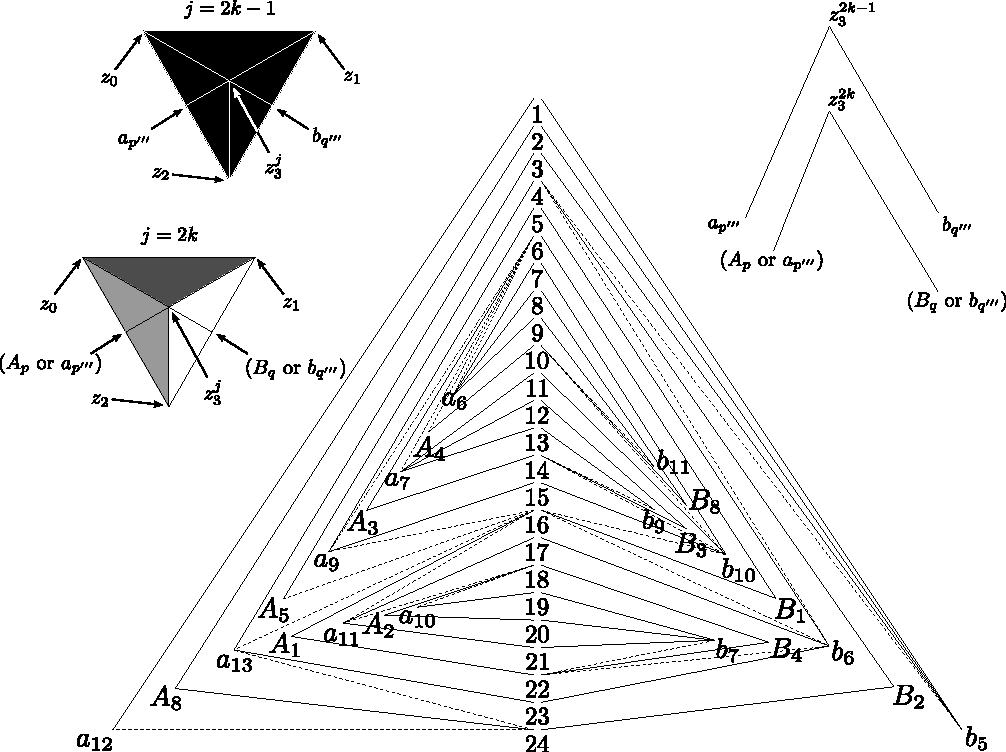
\includegraphics[width=15cm]{A.figs/U.pdf}
\caption{We use the cone construction with the solid lines to obtain $\mathcal{H}_1^\diamond.$ 
Then we use the dashed lines
to obtain the information of $z_3^\dagger$ and $a_{p'}, A_p, a_{p''}$ or $b_{q'}, B_q, b_{q''}$ 
latter when obtaining $\mathcal{L}_i^\star$. Also, we have $p'''\in\{p' ,p''\}$ and  $q'''\in\{q' ,q''\}$.} 
\label{fig:U}
\end{center}
\end{figure}

\begin{proposition}
\label{cor:embedcone}
If $\mathcal{W}_m^h$ is embedded rectilinearly in $\Pi_h$, $h \in \{\ell,r\}$,
then the pair of embeddings can be 
extended to an embedding of $\mathcal{H}^\diamond_1$ into $\mathbb{R}^3$,
via the cone construction.
\end{proposition}
\begin{proof}
 Straighforward from the simple geometry of the situation.
\end{proof}
%--------------------
%\begin{figure}
%\begin{center}
%\includegraphics[scale=1.2]{A.figs/grau.pdf}
%\caption{}
%\label{fig:grau}
%\end{center}
%\end{figure}
%--------------------







% 


\section{Blowing up the tails and
constructing\\ $\mathcal{H}_{2}^\diamond, \mathcal{H}_{3}^\diamond, 
\ldots, \mathcal{H}_{n}^\diamond=\mathcal{H}_{n}^\star$}

The process of replacing the embedded tail of a balloon by the corresponding
trio of PL2-faces in the pillow is denominated \index{blow up a tail} {\em the blowing up of the 
balloon's tail}.

%{\huge \bf Aqui insira seus $\alpha, \beta, \gamma$, bumps, etc}
%\begin{theorem}\label{theo:teoremadeumalinha}
% There is an $O(n)$-algorithm for blowing up a single balloon's tail.
%Thus finding $E\mathcal{L}_n^\star$ and  $E\mathcal{H}_n^\star= 
%E\mathcal{U}_n^\star \cup E\mathcal{L}_n^\star$
%take $O(n^2)$ steps.
%\end{theorem}
\begin{theorem}\label{theo:teoremadeumalinha}
 There is an $O(n)$-algorithm for blowing up a single balloon's tail.
Thus finding $\mathcal{H}_n^\star$ take, $O(n^2)$ steps.
\end{theorem}
\begin{proof}
%Here we get an explicit embedding $E\mathcal{L}_{n}^\star$.
%This finishes the description of $E\mathcal{H}_n^\star.$
%This 2-complex becomes geometrically
%consistent with the combinatorial one in the sense 
%that there are no spurious crossings. 
$\mathcal{H}_{i+1}^\diamond$ is the union of $\mathcal{H}_{i}^\diamond$ with $\mathcal{L}_{i+1}^\star$
and an {\em $\epsilon$-change} in some PL3-faces, if the rank of the type of balloon's tail of the i-th $bp$-move has rank greater than 1
(we call $\epsilon$-change because this change is small, as described below).
At the same time we update the colors of the middle layer to match the colors of the $i$-th pillow in the sequence of $bp$-moves.


%(We proceed the embed of $\mathcal{L}_i^\star$ in the same order as the $bp$-move.
%In each step from $E\mathcal{U}_i^\star$ to $E\mathcal{U}_{i+1}^\star$,
% we change the color of two 2-simplices in the medial layer, of the open balloon's head of this step in $E\mathcal{U}_i^\star$,
%to match with the medial layer of the $bp$-move and embed $\mathcal{L}_i^\star$.
%Basically $E\mathcal{U}_{i+1}^\star$ is the union of $E\mathcal{U}_{i}^\star$ with 
%$E\mathcal{L}_{i}^\star$ and a change of the color in two 2-simplices of $\mathcal{U}_{i}^\star$
%(in some steps we make changes in some tetrahedra which is already embedded to create space to the embed of $\mathcal{L}_i^\star$).
% The final embedding $E\mathcal{U}_n^\star$ is equals to $E\mathcal{H}_n^\star$,
%but $E\mathcal{U}_i^\star \neq E\mathcal{H}_i^\star$ if $i<n.$

Now we describe how to embed each kind of $\mathcal{L}_{i}^\star$ 
(explaining how to $\epsilon$-change some PL3-faces,
to get space for $E\mathcal{L}_i^\star$).


If the balloon's tail is of type $P_1$ (the case $B_1$ is analogous).
Make two copies of $P_1$, resulting in three $P_1$, but change the color of the one which will be in
the middle, and define the 0-simplices like in Fig. \ref{fig:3d2}.

\begin{figure}[!htb] 
\begin{center}
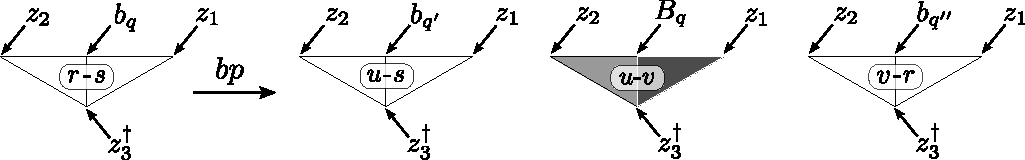
\includegraphics[width=14cm]{A.figs/3d2.pdf}
\caption{Embedding the part of the pillow corresponding to the tail of the balloon: case $P_1$ of the tail.}
\label{fig:3d2}
\end{center}
\end{figure}
If the balloon's tail is of type $B_i$, $i>1$ (the case $P_i$ is analogous).
Make two copies of $B_i$, refine the copies and the original, resulting in three $B_i'$, 
but change the color of the one which will be in
the middle, and define the 0-simplices like in Fig. \ref{fig:3d3}.


The images $\chi_j$ we already know from previous $bp$-move, now we need to define all the images
$\alpha_j, \beta_j$ and $\gamma_j.$
Let $\beta_j$ be $\frac{z_2+\chi_{j+1}}{2}$ 
for each $j=1,\ldots, i$.
As the images $\alpha_j$ and $\gamma_j$ can be defined in analogus way, we just explain how to define each $\alpha_j$.
We know that each $\alpha_j$ is in the PL3-face $\nabla_r$. To 
define each $\alpha_j$ we need 
to reduce the PL3-face $\nabla_r$
in order to get enough space for the PL2-faces of color 0 and 2 of the PL3-faces $\nabla_u$ and $\nabla_v$.
Consider the PL3-face $\nabla_r$, each $\beta_j$ is already defined, so 
define each $\zeta_j$ as $\frac{z_2+\omega_{j+1}}{2}$, where $\omega_k$ is previously defined, %that they are as if we where going to refine
 see Fig. \ref{fig:nextdual3}. Define $\alpha_j$ as $\frac{\zeta_j+\beta_j}{2}$. 

\begin{figure}[!htb] 
\begin{center}
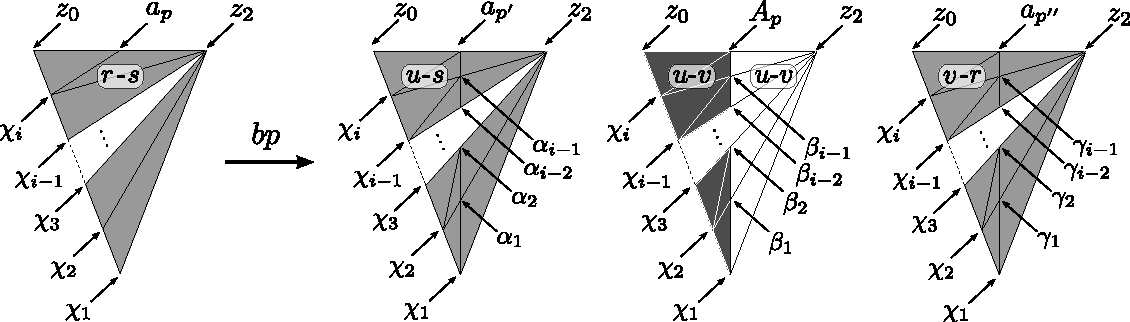
\includegraphics[width=14cm]{A.figs/3d3.pdf}
\caption{Embedding the part of the pillow corresponding to the tail of the balloon: case $B_i$ of the tail.}
\label{fig:3d3}
\end{center}
\end{figure}

\begin{figure}[!htb] 
\begin{center}
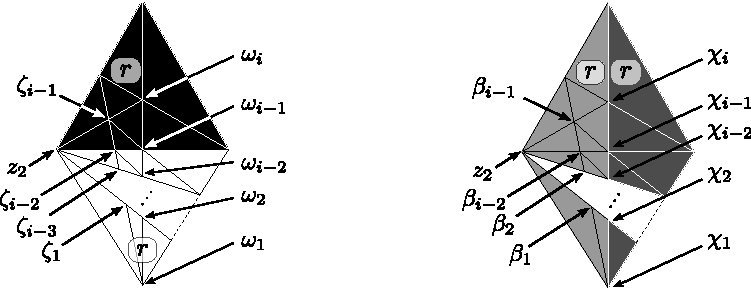
\includegraphics[scale=0.8]{A.figs/nextdual3.pdf}
\caption{Using the PL3-face corresponding to $r$ to define the $\alpha_j$ as $\frac{\zeta_j+\beta_j}{2}$.}
\label{fig:nextdual3}
\end{center}
\end{figure}


The last case is when balloon's tail is refined, that means it is of type $P_i'$ or $B_i'$, $i>1$. We treat the case $B_i'$,
 see Fig. \ref{fig:3d4}. All the 0-simplices $\beta_j$ are already defined, we need to define each
$\alpha_j$ and each $\gamma_j$. Observe that here $r\neq s-1$ and the definitions of $\alpha_j$ and $\gamma_j$ 
are not analogous.

\begin{figure}[!htb] 
\begin{center}
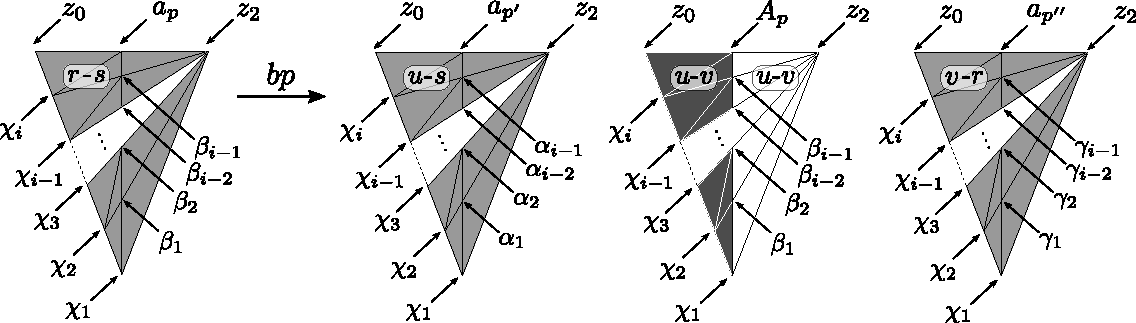
\includegraphics[width=15cm]{A.figs/3d4.pdf}
\caption{Embedding the part of the pillow corresponding to the tail of the balloon: case $B_i'$ of the tail.}
\label{fig:3d4}
\end{center}
\end{figure}


In this case, we need to reduce the PL3-faces $\nabla_r$ and $\nabla_s$
to create enough space to build PL2-faces 0- and 2-colored.
To define 0-simplices $\alpha_j$ and $\gamma_j$, one of these cases is analogous to the case not
 refined, but the other we describe here. ($\nabla_r$ is in the new case is the rank 
%of
%the PL2$_0$- and PL2$_1$-faces of $\nabla_r$, the new case 
%happens when the rank
 of PL2$_0$-face is equals to the rank of the PL2$_1$-face plus 2, if its not true,
the new case is in the PL3-face $\nabla_v$).
Suppose that the new case is in the PL3-face, $\nabla_r$. To define $\alpha_j$,
suppose that the PL2$_0$-face of this PL3-face is not refined,
 see Fig. \ref{fig:3d5}. Define each $\alpha_j$  as the middle point between $\beta_j$ and $\omega_j$.



\begin{figure}[!htb] 
\begin{center}
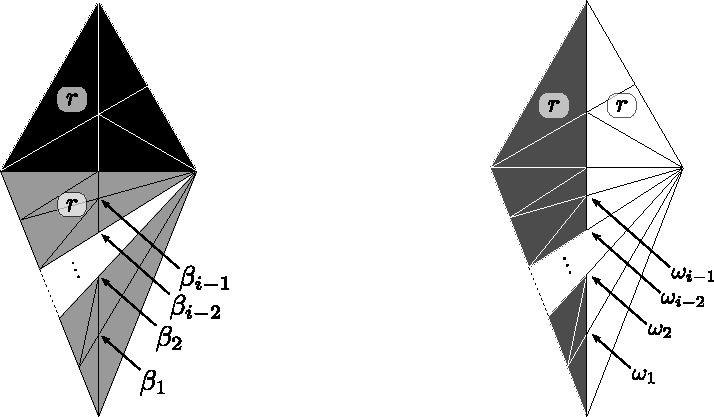
\includegraphics[scale=0.7]{A.figs/3d5.pdf}
\caption{Using the PL3-face $\nabla_r$ to define $\alpha_j$ as $\frac{\omega_j+\beta_j}{2}$.}
\label{fig:3d5}
\end{center}
\end{figure}

Consider the case that the PL2$_0$-face, of the PL3-face $\nabla_r$, is refined
see Fig. \ref{fig:3d6}.
 This is a final subtlety which 
is treated with the {\em bump}. \index{bump} This is characterized by a
non-convex pentagon shown in the bottom part of Fig. \ref{fig:3d6}.
Let $\nu_j$ be $\frac{z_2+\omega_j}{2}$
and $\alpha_j$ as $\frac{\beta_{j-1}+\nu_j}{2}$, for $j=1,\ldots, i-1$. Observe that
if we define $\alpha_j$ as if the PL2$_0$-face
where not refined, some 1-simplices may cross.

%\begin{figure}[!htb] 
%\begin{center}
%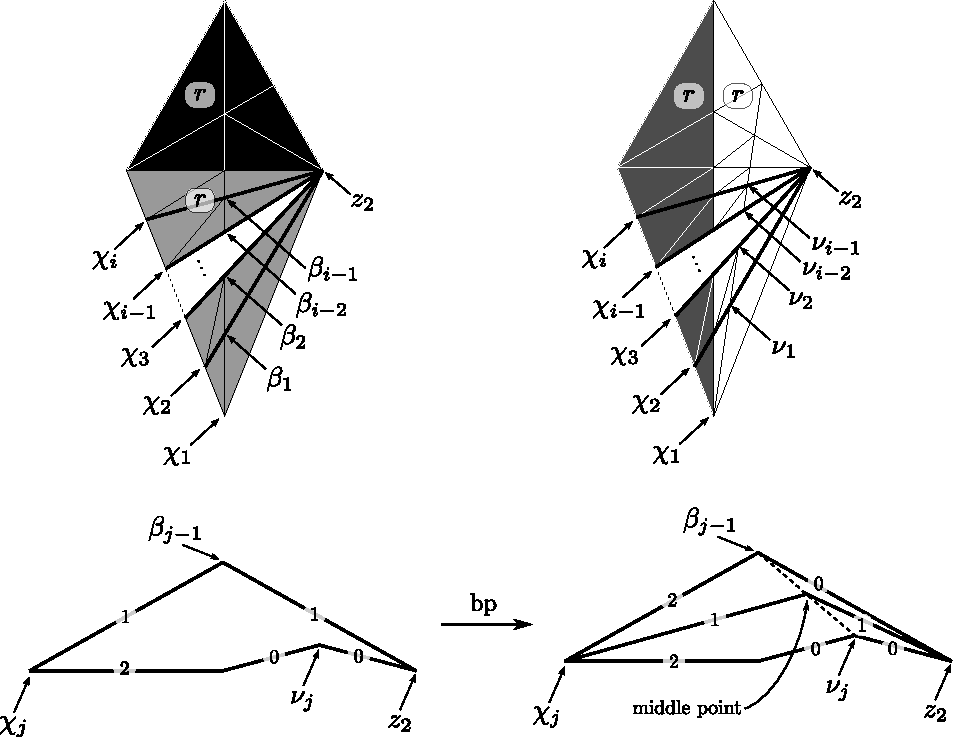
\includegraphics[scale=0.7]{A.figs/3d6.pdf}
%\caption{Using the PL-tetrahedron $\nabla_r$ to define $\alpha_j$ as the middle point between $\mathcal{\nu}_j$ and $\beta_{j-1}$
%(because of the bump, see Fig. \ref{fig:3d7}).}
%The bump: a final dificulty to overcome.}
%\label{fig:3d6}
%\end{center}
%\end{figure}


\begin{figure}[!htb] 
\begin{center}
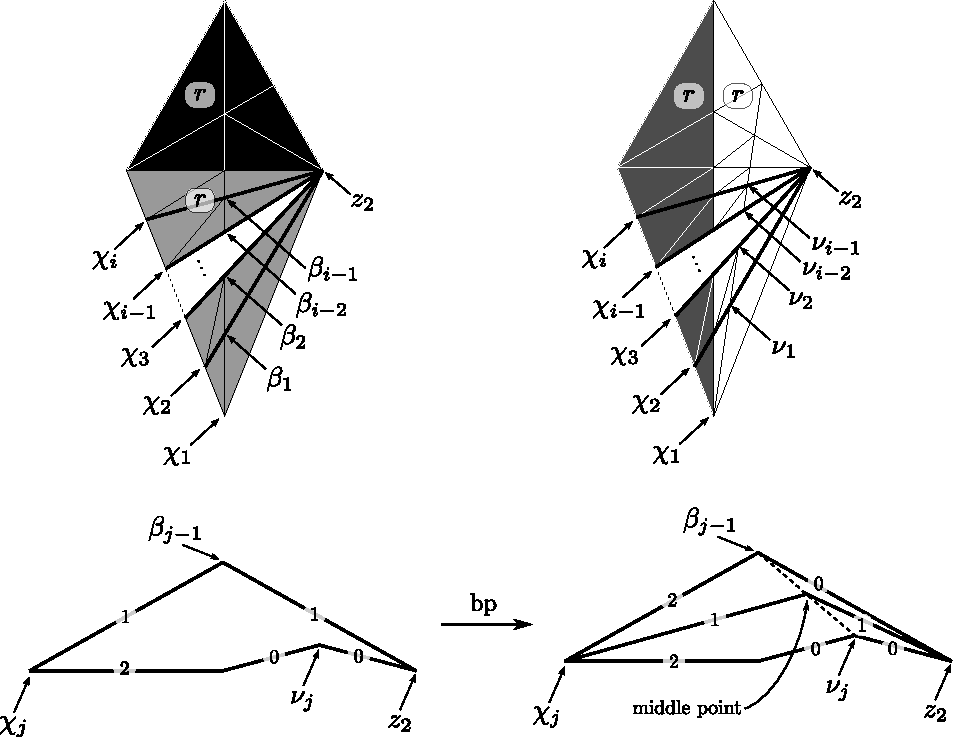
\includegraphics[scale=0.7]{A.figs/3d6.pdf}
\caption{The bump: a final subtlety and how to deal with it.}
\label{fig:3d6}
\end{center}
\end{figure}

\end{proof}

% 



\section{Obtaining the framed Link}
Given $\mathcal{H}_{n}^\star$ into
$\mathbb{R}^3$ we obtain the $k$-component 
framed link (corresponding to the $k$ twistors) as a set of 
PL-triangulated $k$ cylinders in the 2-skeleton of 
$\mathcal{H}_{n}^\star$, named $\mathcal{C}_1,$ $\mathcal{C}_2, \ldots,\mathcal{C}_k$.
Observe that at this stage every 0-simplex of  $\bigcup_{j=1}^k \mathcal{C}_j$ 
has a 3-D coordinate attached to it. These cylinders are parametrized
as $k$ pairs of isometric rectangles (forming a strip) as in Fig. \ref{fig:strips}.
We draw $k$ straight horizontal lines at different heights of the rectangles, in the example,
lines $c_1-c_1$, $c_2-c_2$ and $c_3-c_3$. These lines are 
mapped into polygons in $\mathbb{R}^3$ which are PL-closed curves. 
The data we need is $\bigcup_{j=1}^k \mathcal{C}_j \subset \mathcal{H}_{n}^\star$
and we can discard the rest of $\mathcal{H}_{n}^\star$. The link that we seek 
is $\bigcup_{j=1}^k c_j$ with framing $\ell_j$, where $\ell_j$ is
given by the linking number of the two components of $\mathcal{C}_j$ oriented in
the same (arbitrary) direction.
We briefly review the definition of linking number 
\cite {lickorish1997introduction}.
Consider two distinct components $K_1$ and $K_2$ of an oriented link projected into
the plane so that the crossings are transversal 
(no tangency) and that there are no triple points. 
The projection is also {\em decorated}
in the sense that at each crossing the upper and 
the lower strands are given, usually,
by omitting a small segment of the lower strand.
 The \index{linking number} {\em linking number} of $\{K_1, K_2\}$
is half of the algebraic sum of the signs of the crossings 
between $K_1$ and $K_2$, oriented 
in the same direction. If $G$ is a gem, $|G|$ means
the 3-manifold induced by $G$.
The link projection given in Fig. \ref{fig:projecoes2} 
which induce $|r^{24}_5|$ has its three linking numbers $-3$.




%----------------------


\begin{proposition}
\label{prop:totalnumberofsimplices}
 The number of 1-simplices in $\bigcup_{j=1}^k c_j$ is 
at most $12n^2$, where $2n$ is the number
of vertices of the input gem.
\end{proposition}
\begin{proof} 
 A $c_j$ crosses one PL2$_m$-face, for $m\in \{0,1,2,3\}$.
 It is easy to verify that the maximum number of 2-simplices in $B_i'$ or $ P'_i$ is
 $3i-1$ and this number exceeds similar numbers for $B_i$, $ P_i$, $R^b_i$ and $R^p_i$, for 
 $i \ge  1$. The maximum $i$ is $2n-1$, so the maximum number of 2-simplices 0-, 1- and 2-colored in one PL2-face of the 
 final complex is $6n-4$. Each 1-simplex of $c_j$ crosses at most once each 2-simplex.
 Therefore, the number of 1-simpices crossing a 2-simplex 0-, 1- and 2-colored is at most $12n-8$. 
 A $c_j$ crosses at most four 2-simplices 3-colored. The result follows because $n$ is an upper 
 bound for $k$, number of components. Just note that a component in the link
 is in 1-1 correspondence with the twistors of the original gem and a twistor 
is formed by 2 vertices. This proof is partially ilustrated in Fig. \ref{fig:strips}.
 The illustration is not faithful because we can replace the strips at the right by
their bottom parts, getting simpler cylinders homotopic to the ones illustrated.
\end{proof}

Each cylinder is formed by two strips. Each strip by two adequate
pairs of two PL2-faces in the boundary of the PL3-faces in the hinge.
In the way depicted we have one PL3-face of each color $c$, $c=0,1,2,3$.
The number of  crossings of the curves $c_j$, $j=1,2,3$ coincides with the
number of $1$-simplices (or $0$-simplices) of $\bigcup_{j=1}^3 \mathcal{C}_j$.
To decrease this number we can replace the part of the strip which does not use a
PL2$_3$-face by the two complementary PL2$_3$-faces in the corresponding PL3-face.
This produces isotopic cylinders, but the number of crossings of the $c_j$'s are smaller. 
Note that each PL2$_3$-face has just five 2-simplices. In Fig. \ref{fig:strips} we 
depict the situation for the wings arising from $r_5^{24}$ before the 3 replacements.


\begin{figure}[!htb]
\begin{center}
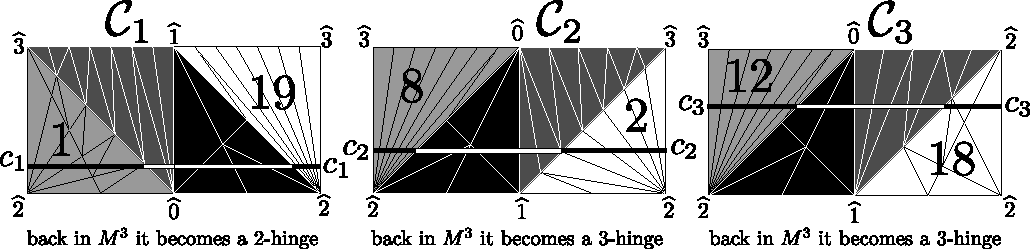
\includegraphics[width=15cm]{A.figs/strips.pdf}
\caption{From hinges to cylinders 
$\mathcal{C}_j$  to curves  $c_j$ (example inducing  $|r^{24}_5|$).
%Each cylinder is formed by two strips. Each strip by two adequate
%pairs of two PL2-faces in the boundary of the PL3-faces in the hinge.
%In the way depicted we have one PL3-face of each color $c$, $c=0,1,2,3$.
%The number of  crossings of the curves $c_j$, $j=1,2,3$ coincides with the
%number of $1$-simplices (or $0$-simplices) of $\bigcup_{j=1}^3 \mathcal{C}_j$.
%To decrease this number we can replace the right part of each strip by the
%two complementary faces at each right PL3-face. This produce isotopic cylinders,
%but the number of crossings of the $c_j$'s are smaller.
}  
\label{fig:strips}
\end{center}
\end{figure}

%----------------------
\begin{figure}[!htb]
\begin{center}
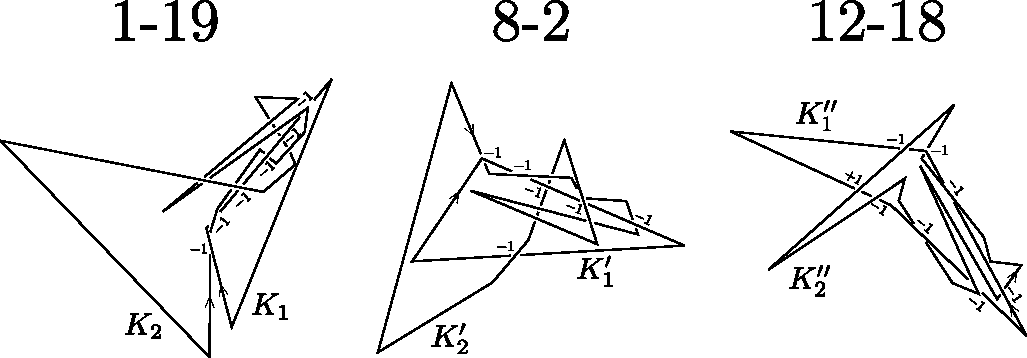
\includegraphics[scale=0.9]{A.figs/projecoes2.pdf}
\caption{Projection of the algorithm's output, yielding 
the linking numbers of the 
boundary components of the embedded cylinders of Fig. \ref{fig:strips}.}
\label{fig:projecoes2}
\end{center}
\end{figure}





% 



\section{Obtaining a Gauss code for the link}

At this point, we have the link as a set of cyclic sequences of points in $\mathbb{R}^3$.
We also have the framing of each component. Thus the theoretical problem is solved. 
However, it is convenient to go on getting adequate planar projections to produce 
planar diagram for the link.
We obtain the following Gauss code, 
(\cite{rosenstiehl1976solution}, chapter 3 of \cite{Lins1980}, 
\cite{lins2008hsg}),
where signs mean
up $(+)$ and down $(-)$ passages:
$ ((-2,+3, -4,+1), (-5, +6, +2, -1),$ $(-3, +4, -7, -6, +5, +7)).$
From this code we get the link planar diagram of 
Figs. \ref{fig:r24_5link2}.
Since we have the framings curls
can be removed. An explicit elegant framed link inducing the euclidean 
3-manifold $|r^{24}_5|$ was previously unknown. We use 
Fig. \ref{fig:r24_5link} as input for L. Lins's software \cite{lins2007blink} to obtain
the WRT-invariants from $r=3$ to $r=20$ for the space $|r^{24}_5|$. We also apply our algorithm
for the Weber-Seifert hyperbolic dodecahedron space, obtaining a link with
142 crossings, included in Appendix B.

\begin{figure}[!htb]
\begin{center}
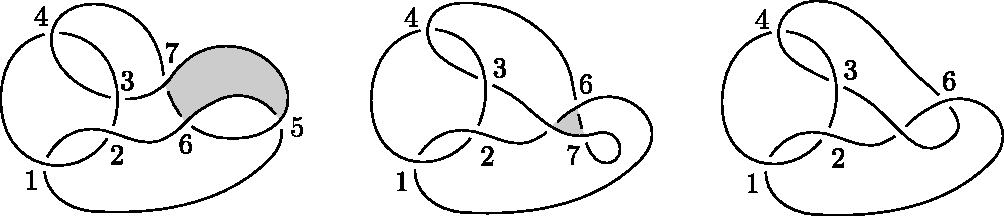
\includegraphics[width=12cm]{A.figs/r24_5link2.pdf}
\caption{Simplifying the link diagram for $|r_5^{24}|$.}
\label{fig:r24_5link2}
\end{center}
\end{figure}


\begin{figure}[!htb]
\begin{center}
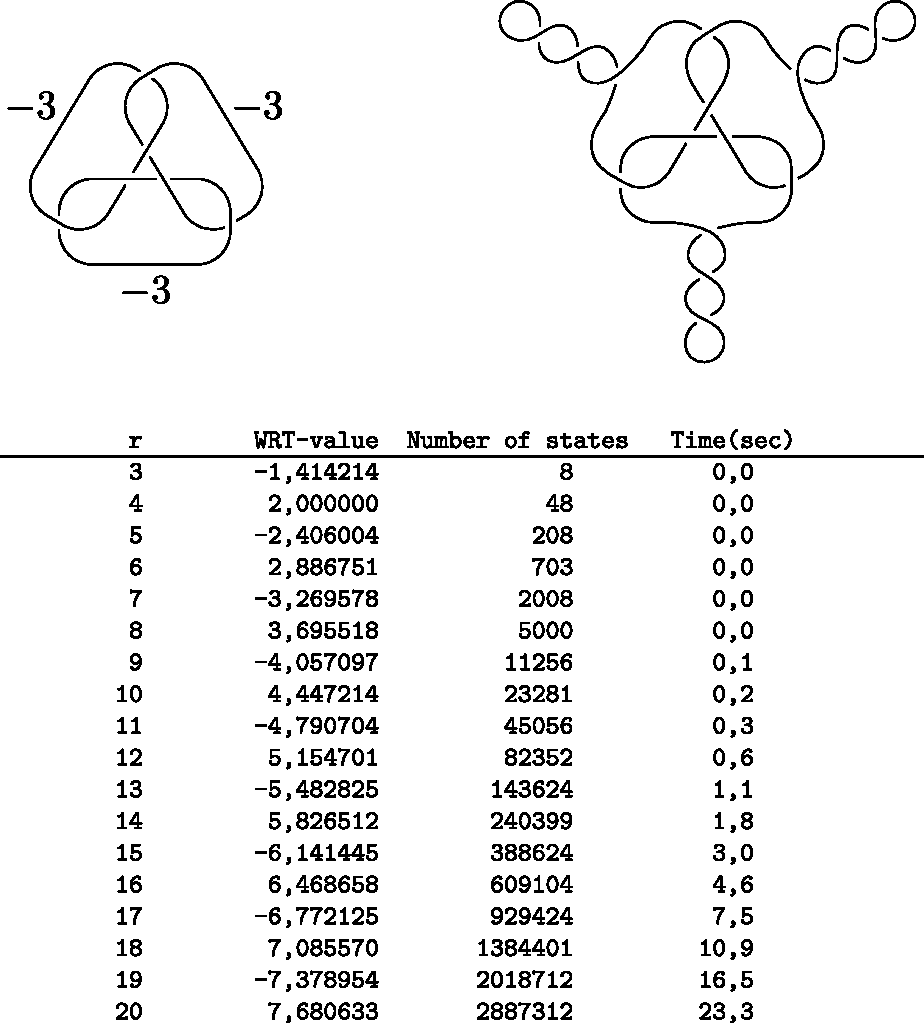
\includegraphics[width=11cm]{A.figs/r24_5link.pdf}
\caption{Framed link, blackboard framed link and WRT-invariants for $|r_5^{24}|$.
 %These invariants assume real values because the space is symmetric: the two
%oriented forms agree.
 Data obtained from L. Lins software \cite{lins2007blink}.}
\label{fig:r24_5link}
\end{center}
\end{figure}

%\begin{figure}[!htb]
%\begin{center}
%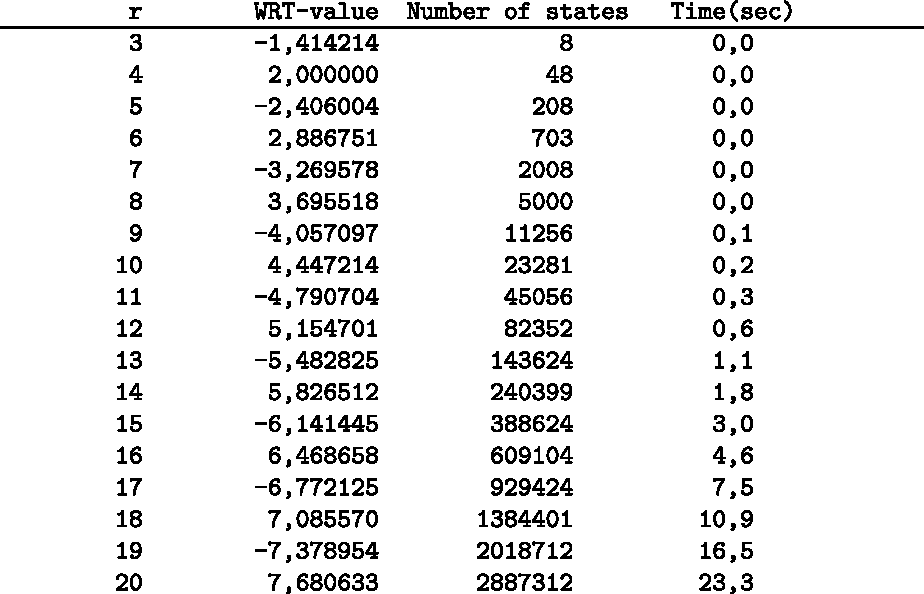
\includegraphics[width=13cm]{A.figs/r24_5linkinvariants.pdf}
%\caption{ WRT-invariants for $|r_5^{24}|$.
% These invariants assume real values because the space is symmetric: the two
%oriented forms agree. Data obtained from L. Lins software \cite{lins2007blink}.}
%\label{fig:r24_5link}
%\end{center}
%\end{figure}

\newpage
\begin{algorithm}
\label{theo:algorithm}
 There exists an $O(n^2)$-algorithm to produce, from a
  resoluble gem inducing an $M^3$,  a blackboard framed link also inducing $M^3$.
\end{algorithm}
\begin{proof} 
We start with a resoluble gem $G$ with $2n$ vertices. Here is the algorithm,
justified by the theory previously developed:
\begin{itemize}
 \item Form decreasing sequence of gems starting with $\mathcal{J}^2$,
 the $J^2$-gem associated with
the resolution of $G$ performing adequate $0$- or $1$-flips
 and finishing at the bloboid $\mathcal{B}_1$:
$\mathcal{J}^2=\mathcal{H}_{n},  \mathcal{H}_{n-1}, \ldots, \mathcal{H}_1=\mathcal{B}_1$.
%See Fig. \ref{fig:j2gemrSEQ} for the $r^{24}_5$-example.
 
 \item Form sequence of balloons $\mathcal{B}_1^\star,\ldots, \mathcal{B}_{n-1}^\star$
and pillows $\mathcal{P}_2^\star,\ldots, \mathcal{P}_n^\star$ defining implicitly the 
  sequence of combinatorial $2$-complexes $\mathcal{H}_1^\star, \mathcal{H}_1^\star, 
\ldots, \mathcal{H}_{2n}^\star$, together with 
their respective wings and nervures (combinatorially   
given by rotations), 
$\mathcal{W}_1^\ell \cup \mathcal{N}_1^\ell$, 
$\mathcal{W}_2^\ell \cup \mathcal{N}_2^\ell$,
\ldots, $\mathcal{W}_n^\ell \cup \mathcal{N}_n^\ell$ and 
$\mathcal{W}_1^r \cup \mathcal{N}_1^r$, 
$\mathcal{W}_2^r \cup \mathcal{N}_2^r$,
\ldots, $\mathcal{W}_n^r \cup \mathcal{N}_n^r$.
Each $bp$-move is simply a flip in the
primal sequence. See Figs. \ref{fig:winglist01} to \ref{fig:winglist11}
from the $r^{24}_5$-example.

\item Use Tutte's barycentric method with the edge weight 
heuristic (Fig. \ref{fig:arvorecompesos} from the $r^{24}_5$-example) 
to provide rectilinear embeddings
of $\mathcal{W}_n^\ell \cup \mathcal{N}_n^\ell$ in $\Pi_\ell$ and
of $\mathcal{W}_n^r \cup \mathcal{N}_n^r$ in $\Pi_r$ fixing the outer regions.
The nervures
are useful up to this point, and after obtaining the rectilinear embeddings
they can be discarded.

\item Get $\mathcal{H}_{1}^\diamond$ using
$\mathcal{W}_n^\ell \cup \mathcal{W}_n^r$ 
by the cone construction.


\item Get the sequence $\mathcal{H}_{2}^\diamond, \ldots, \mathcal{H}_{n}^\diamond = \mathcal{H}_n^\star$
by the blowing up technique in the proof of Theorem \ref{theo:teoremadeumalinha}.

\item Define the framings of the components of the link
as the linking numbers of the boundaries of the cylinders formed by
the strips coming from the hinges; special care: distinguish the
hinges which become 2-hinges from the
hinges which become 3-hinges in $M^3$. See Fig. \ref{fig:strips}.

\item Find an adequate projection of suitable medial curves in the cylinders.
These curves form the link. Find Gauss code for the link, and so,
a projection is combinatorially specified (\cite{rosenstiehl1976solution}, 
chapter 3 of \cite{Lins1980}, 
\cite{lins2008hsg}). Add curls to produce
a blackboard framed link. See Figs. \ref{fig:r24_5link2} and \ref{fig:r24_5link}
from the $r^{24}_5$-example.
\end{itemize}
This algorithm has both space complexity and time complexity $O(n^2)$.
Its output, first obtained as a set with no more than $n$ 
PL-polygons in $\mathbb{R}^3$,  
has a total of at most $12n^2$ vertices.
\end{proof}


%\chapter{Table of QI of spaces EUCLID$_i$}

%\section{EUCLID$_0$: Rep. $r_1^{24}$}

%\begin{figure}[!htb]
%\begin{center}
%\includegraphics[width=10.5cm]{A.figs/r24-1.pdf}
%\caption{3-gem, blackboard framed link for $|r_1^{24}|$ and
%WRT-invariants.}
%\label{fig:r24_5link}
%\end{center}
%\end{figure}

%\newpage

%\section{EUCLID$_1$: Rep. $r_5^{24}$}

%\begin{figure}[!htb]
%\begin{center}
%\includegraphics[width=10.5cm]{A.figs/r24_5GemLinkWRT.pdf}
%\caption{3-gem, blackboard framed link for $|r_5^{24}|$ and
%WRT-invariants.}
%\label{fig:r24_5link}
%\end{center}
%\end{figure}

%\newpage

%\section{EUCLID$_3$: Rep. $r_6^{24}$}%

%\begin{figure}[!htb]
%\begin{center}
%\includegraphics[width=10.5cm]{A.figs/r24_6.pdf}
%\caption{3-gem, blackboard framed link for $|r_6^{24}|$ and
%WRT-invariants.}
%\label{fig:r24_5link}
%\end{center}
%\end{figure}

%-----------------------------------

%\bibliographystyle{is-alpha}
%\addcontentsline{toc}{bibliografia}{\MakeTextUppercase{Refer�ncias Bibliogr�ficas}}
%\bibliography{d:/slsl\3.DadosSostenes.35.ArtigosLivros.bibtexGoogleScholar/bibtexIndex.bib} % bib file is slsl.bib
%\bibliography{~/home/ricardo/Dropbox/35.ArtigosLivros.bibtexGoogleScholar/bibtexIndex.bib}
%\bibliography{bibtexIndex.bib}
%\bibliography{slsl}

% \printindex
-----------


%\section{Appendix A: Proofs}\label{appA}

%\begin{proposition}
%\label{prop:planetwist}
%Let $G$ be a gem. $(a)$ A $ji$-twisting of a $j$-twistor of $G$ is factorable as
%one $i$-flip and one $j$-flip.
%$(b)$ If $G$ has a $0$-consecutive labelling on its vertices,
%then a $ji$-twisting can be accomplished by one $k$-flip (which maintains planarity
%of the $\widehat{0}$-residue) followed
%by the $\{u,v\}$ label interchange. The final gem has a $0$-consecutive labelling
%and so the $ji$-twisting is entirely depicted in the $\widehat{0}$-residue,
%a plane graph.
%\end{proposition}

%\begin{proof}\hspace{-4mm} ({\bf Theorem \ref{theo:bound}})
%The proof is provided at the end of the paper, as Algorithm
%\ref{theo:algorithm}.
%\end{proof}


\section*{Appendix A: a solution for the 
Weber-Seifert Dodecahedral Hyperbolic Space}

We found a projection for a framed link with 142 crossings for the 
Weber-Seifert Dodecahedral Hyperbolic Space. Actually the PL-link are nine PL-polygons in
$\mathbb{R}^3$ with a total of only 68 vertices.
The data that follows is a positive answer for Jeffrey Weeks' question more than
twenty years ago. Still in raw form, it can be substantially simplified

We apply our algorithm to the 50-vertex gem 
and its resolution given at the right side of Fig. 
\ref{fig:resolutionDhip50A}. 

%-----------------------------------
\begin{figure}[!htb]
\begin{center}
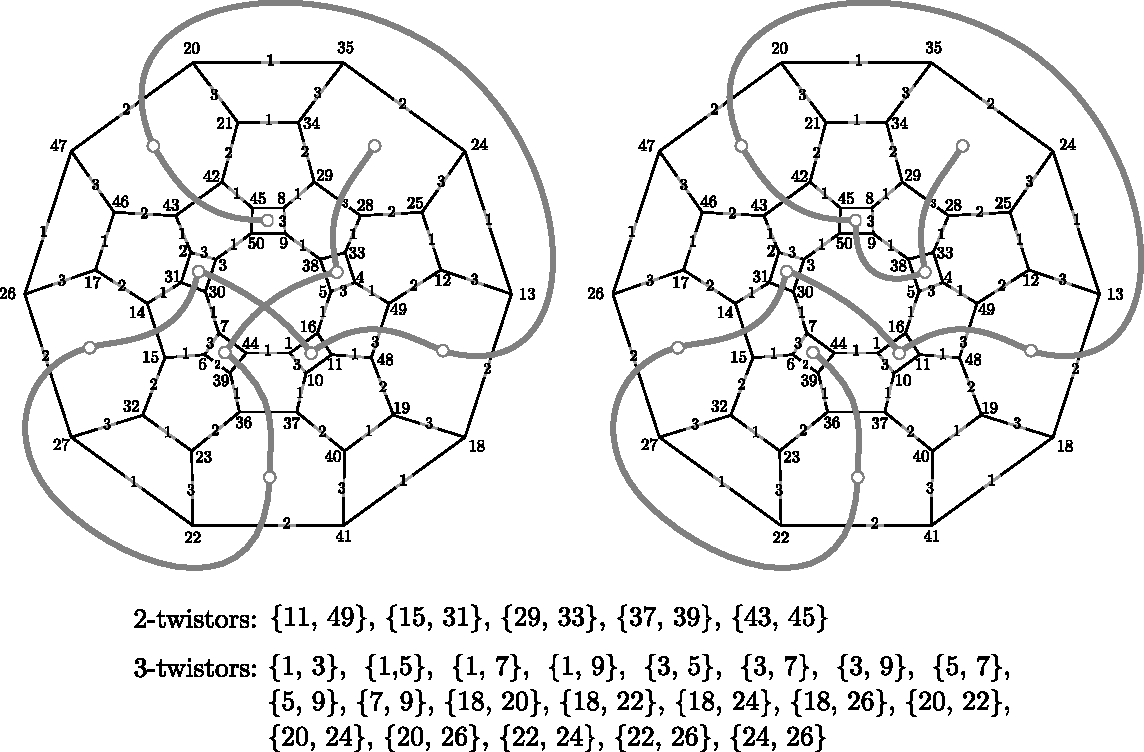
\includegraphics[width=14.5cm]{A.figs/resolutionDhip50A.pdf} \\
\caption{\sf This is a 50-vertex gem which behaves as the {\em attractor}.}
%(see \cite{lins1995gca})
%for the Weber-Seifert dodecahedral hyperbolic space.
%For a proof that it induces this space see also \cite{lins1995gca}.} 
\label{fig:resolutionDhip50A}
\end{center}
\end{figure}
%-----------------------------------

A crossing $x\in \mathbb{N}$ has 4 legs in counterclockwise 
order: $(4x-3, 4x-2, 4x-1, 4x)$.
A {\em duet} \index{duet} is a perfect matching of the legs.
The first entry of a \index{quintet} {\em quintet} is the number of the crossing.
Each crossing appears in two consecutive quintets. The second entry is $d$ 
or $u$ depending on whether the quintet holds the first or the second occurrence
of its crossing. The $d$ means that the southwest to the northeast passage
goes under, the $u$ means that it goes over. The third and fourth entries of a quintet
are legs and their order specifies a consistent orientation for all the components
of the link. The fifth and last entry of a quintet is the number of the component
of the link that contains the two legs. By properly embedding the quintets in the plane
and identifying the legs as specified by the duets we have a link diagram
with consistent orientation of all of its component. Thus to obtain a Gauss code
(\cite{rosenstiehl1976solution}, chapter 3 of \cite{Lins1980}, 
\cite{lins2008hsg}), for the link is straightforward. 
Even though 
there are 142 crossings in the projection, the number of 1-simplices
in the PL-link is only 68. This was obtained by a shortcutting technique 
which started with over two hundred 1-simplices:
each 0-simplex defines a triangle in $\mathbb{R}^3$; if this triangle
is not pierced by a 1-simplex, then the 0-simplex is removed from the link. 
Compare 68 with our theoretical 
bound, namely $12n^2=7500$, since $n=25$. We emphasize the issue that
the algorithm behaves very efficiently. 


\subsection{Duets of $DHIP_{50}^{142}$}
{\scriptsize
\begin{center}
$
\begin{array}{|c|c|c|c|c|c|c|c|} \hline
 1, 8 &
 2, 155 &
 3, 112 &
 4, 111 &
 5, 108 &
 6, 11 &
 7, 104 &
 9, 16 \\
 10, 101&
 12, 107&
 13, 564&
 14, 19&
 15, 102&
 17, 24&
 18, 97&
 20, 159 \\
 21, 158&
 22, 27&
 23, 468&
 25, 32&
 26, 465&
 28, 163&
 29, 340&
 30, 35 \\
 31, 336&
 33, 40&
 34, 267&
 36, 271&
 37, 560&
 38, 43&
 39, 268&
 41, 48 \\
 42, 75&
 44, 559&
 45, 72&
 46, 51&
 47, 76&
 49, 56&
 50, 495&
 52, 71 \\
 53, 68&
 54, 59&
 55, 188&
 57, 62&
 58, 185&
 60, 63&
 61, 500&
 64, 67 \\
 65, 70&
 66, 183&
 69, 184&
 73, 494&
 74, 79&
 77, 84&
 78, 263&
 80, 259 \\
 81, 258&
 82, 85&
 83, 26&
 86, 475&
 87, 92&
 88, 335&
 89, 472&
 90, 93 \\
 91, 466&
 94, 471&
 95, 98&
 96, 467&
 99, 156&
 100, 103&
 105, 110&
 106, 319 \\
 109, 320&
 113, 240&
 114, 239&
 115, 526&
 116, 117&
 118, 525&
 119, 122&
 120, 235 \\
 121, 236&
 123, 142&
 124, 127&
 125, 132&
 126, 531&
 128, 139&
 129, 136&
 130, 135 \\
 131, 532&
 133, 138&
 134, 317&
 137, 230&
 140, 141&
 143, 146&
 144, 231&
 145, 524 \\
 147, 528&
 148, 149&
 150, 527&
 151, 154&
 152, 383&
 153, 244&
 157, 164&
 160, 563 \\
 161, 464&
 162, 167&
 165, 172&
 166, 337&
 168, 463&
 169, 344&
 170, 175&
 171, 338 \\
 173, 180&
 174, 269&
 176, 275&
 177, 556&
 178, 181&
 179, 558&
 182, 497&
 186, 191 \\
 187, 496&
 189, 196&
 190, 489&
 192, 427&
 193, 432&
 194, 199&
 195, 488&
 197, 204 \\
 198, 435&
 200, 431&
 201, 448&
 202, 207&
 203, 544&
 205, 212&
 206, 443&
 208, 447 \\
 209, 446&
 210, 215&
 211, 538&
 213, 220&
 214, 483&
 216, 371&
 217, 370&
 218, 223 \\
 219, 376&
 221, 226&
 222, 373&
 224, 311&
 225, 522&
 227, 316&
 228, 229&
 232, 523 \\
 233, 530&
 234, 237&
 238, 529&
 241, 470&
 242, 247&
 243, 324&
 245, 252&
 246, 321 \\
 248, 327&
 249, 326&
 250, 253&
 251, 568&
 254, 329&
 255, 260&
 256, 479&
 257, 332 \\
 261, 334&
 262, 265&
 266, 333&
 270, 557&
 272, 339&
 273, 280&
 274, 553&
 276, 507 \\
 277, 506&
 278, 283&
 279, 416&
 281, 288&
 282, 413&
 284, 411&
 285, 552&
 286, 291 \\
 287, 504&
 289, 296&
 290, 295&
 292, 359&
 293, 364&
 294, 299&
 297, 304&
 298, 365 \\
 300, 363&
 301, 452&
 302, 305&
 303, 366&
 306, 451&
 307, 312&
 308, 369&
 309, 396 \\
 310, 313&
 314, 395&
 315, 318&
 322, 567&
 323, 392&
 325, 330&
 328, 473&
 331, 476 \\
 341, 404&
 342, 347&
 343, 408&
 345, 352&
 346, 511&
 348, 403&
 349, 516&
 350, 353 \\
 351, 512&
 354, 515&
 355, 360&
 356, 551&
 357, 514&
 358, 361&
 362, 519&
 367, 372 \\
 368, 445&
 374, 379&
 375, 484&
 377, 382&
 378, 535&
 380, 521&
 381, 536&
 384, 387 \\
 385, 390&
 386, 565&
 388, 391&
 389, 566&
 393, 456&
 394, 399&
 397, 402&
 398, 459 \\
 400, 455&
 401, 460&
 405, 510&
 406, 409&
 407, 508&
 410, 549&
 412, 505&
 414, 503 \\
 415, 420&
 417, 502&
 418, 421&
 419, 554&
 422, 501&
 423, 428&
 424, 499&
 425, 430 \\
 426, 429&
 433, 440&
 434, 485&
 436, 543&
 437, 542&
 438, 441&
 439, 546&
 442, 541 \\
 444, 537&
 449, 518&
 450, 453&
 454, 517&
 457, 462&
 458, 561&
 461, 562&
 469, 474 \\
 477, 482&
 478, 533&
 480, 539&
 481, 534&
 486, 545&
 487, 490&
 491, 548&
 492, 493 \\
 498, 555&
 509, 550&
 513, 520&
 540, 547 & & & & \\ \hline
\end{array}
$
\end{center}
}



%\subsection{Cylinders and framings}
%\begin{verbatim}
%boundary cylinder 1 linking number from 2-twistor {19,13} is -1
%boundary cylinder 2 linking number from 2-twistor {3,29} is 0
%boundary cylinder 3 linking number from 2-twistor {49,33} is -1
%boundary cylinder 4 linking number from 2-twistor {39,43} is -1
%boundary cylinder 5 linking number from 2-twistor {9,23} is -2
%boundary cylinder 6 linking number from 3-twistor {1,31} is 0
%boundary cylinder 7 linking number from 3-twistor {6,26} is 0
%boundary cylinder 8 linking number from 3-twistor {46,36} is 0
%boundary cylinder 9 linking number from 3-twistor {11,21} is 0
%\end{verbatim}


\subsection{Quintets, cylinders and framings of $DHIP_{50}^{142}$}


{\tiny
\begin{center}
$
\begin{array}{cccccc}
 \{1,\text{d},3,1,1\} & \{1,\text{u},4,2,3\} &
 \{2,\text{d},7,5,8\} & \{2,\text{u},8,6,1\} &
 \{3,\text{d},11,9,1\} & \{3,\text{u},10,12,1\} \\
 \{4,\text{d},13,15,8\} & \{4,\text{u},16,14,1\} &
 \{5,\text{d},18,20,2\} & \{5,\text{u},19,17,1\} &
 \{6,\text{d},24,22,1\} & \{6,\text{u},21,23,9\} \\
 \{7,\text{d},27,25,1\} & \{7,\text{u},28,26,5\} &
 \{8,\text{d},32,30,1\} & \{8,\text{u},31,29,4\} &
 \{9,\text{d},35,33,1\} & \{9,\text{u},34,36,3\} \\
 \{10,\text{d},39,37,9\} & \{10,\text{u},40,38,1\} &
 \{11,\text{d},42,44,8\} & \{11,\text{u},43,41,1\} &
 \{12,\text{d},48,46,1\} & \{12,\text{u},45,47,1\} \\
 \{13,\text{d},51,49,1\} & \{13,\text{u},50,52,6\} &
 \{14,\text{d},53,55,2\} & \{14,\text{u},56,54,1\} &
 \{15,\text{d},59,57,1\} & \{15,\text{u},60,58,8\} \\
 \{16,\text{d},61,63,8\} & \{16,\text{u},62,64,1\} &
 \{17,\text{d},66,68,2\} & \{17,\text{u},67,65,1\} &
 \{18,\text{d},70,72,1\} & \{18,\text{u},71,69,6\} \\
 \{19,\text{d},73,75,8\} & \{19,\text{u},76,74,1\} &
 \{20,\text{d},80,78,4\} & \{20,\text{u},79,77,1\} &
 \{21,\text{d},84,82,1\} & \{21,\text{u},81,83,3\} \\
 \{22,\text{d},86,88,9\} & \{22,\text{u},85,87,1\} &
 \{23,\text{d},91,89,9\} & \{23,\text{u},92,90,1\} &
 \{24,\text{d},93,95,1\} & \{24,\text{u},96,94,5\} \\
 \{25,\text{d},99,97,2\} & \{25,\text{u},98,100,1\} &
 \{26,\text{d},102,104,8\} & \{26,\text{u},103,101,1\} &
 \{27,\text{d},108,106,8\} & \{27,\text{u},107,105,1\} \\
 \{28,\text{d},109,111,3\} & \{28,\text{u},110,112,1\} &
 \{29,\text{d},115,113,6\} & \{29,\text{u},114,116,2\} &
 \{30,\text{d},120,118,8\} & \{30,\text{u},117,119,2\} \\
 \{31,\text{d},123,121,2\} & \{31,\text{u},122,124,2\} &
 \{32,\text{d},126,128,6\} & \{32,\text{u},127,125,2\} &
 \{33,\text{d},129,131,8\} & \{33,\text{u},132,130,2\} \\
 \{34,\text{d},135,133,2\} & \{34,\text{u},134,136,8\} &
 \{35,\text{d},138,140,2\} & \{35,\text{u},139,137,6\} &
 \{36,\text{d},141,143,2\} & \{36,\text{u},144,142,2\} \\
 \{37,\text{d},146,148,2\} & \{37,\text{u},145,147,6\} &
 \{38,\text{d},149,151,2\} & \{38,\text{u},150,152,8\} &
 \{39,\text{d},154,156,2\} & \{39,\text{u},155,153,3\} \\
 \{40,\text{d},159,157,2\} & \{40,\text{u},160,158,9\} &
 \{41,\text{d},164,162,2\} & \{41,\text{u},161,163,5\} &
 \{42,\text{d},167,165,2\} & \{42,\text{u},166,168,8\} \\
 \{43,\text{d},172,170,2\} & \{43,\text{u},171,169,4\} &
 \{44,\text{d},175,173,2\} & \{44,\text{u},174,176,3\} &
 \{45,\text{d},179,177,9\} & \{45,\text{u},180,178,2\} \\
 \{46,\text{d},181,183,2\} & \{46,\text{u},184,182,6\} &
 \{47,\text{d},188,186,2\} & \{47,\text{u},185,187,8\} &
 \{48,\text{d},192,190,7\} & \{48,\text{u},191,189,2\} \\
 \{49,\text{d},196,194,2\} & \{49,\text{u},195,193,7\} &
 \{50,\text{d},200,198,5\} & \{50,\text{u},199,197,2\} &
 \{51,\text{d},204,202,2\} & \{51,\text{u},203,201,7\} \\
 \{52,\text{d},207,205,2\} & \{52,\text{u},206,208,5\} &
 \{53,\text{d},209,211,7\} & \{53,\text{u},212,210,2\} &
 \{54,\text{d},214,216,8\} & \{54,\text{u},215,213,2\} \\
 \{55,\text{d},217,219,4\} & \{55,\text{u},220,218,2\} &
 \{56,\text{d},222,224,5\} & \{56,\text{u},223,221,2\} &
 \{57,\text{d},226,228,2\} & \{57,\text{u},227,225,6\} \\
 \{58,\text{d},230,232,6\} & \{58,\text{u},229,231,2\} &
 \{59,\text{d},233,235,8\} & \{59,\text{u},236,234,2\} &
 \{60,\text{d},237,239,2\} & \{60,\text{u},240,238,6\} \\
 \{61,\text{d},244,242,3\} & \{61,\text{u},241,243,9\} &
 \{62,\text{d},247,245,3\} & \{62,\text{u},246,248,4\} &
 \{63,\text{d},251,249,9\} & \{63,\text{u},252,250,3\} \\
 \{64,\text{d},253,255,3\} & \{64,\text{u},254,256,5\} &
 \{65,\text{d},257,259,4\} & \{65,\text{u},260,258,3\} &
 \{66,\text{d},263,261,4\} & \{66,\text{u},264,262,3\} \\
 \{67,\text{d},266,268,9\} & \{67,\text{u},265,267,3\} &
 \{68,\text{d},270,272,8\} & \{68,\text{u},271,269,3\} &
 \{69,\text{d},276,274,8\} & \{69,\text{u},275,273,3\} \\
 \{70,\text{d},279,277,6\} & \{70,\text{u},280,278,3\} &
 \{71,\text{d},284,282,5\} & \{71,\text{u},283,281,3\} &
 \{72,\text{d},287,285,9\} & \{72,\text{u},288,286,3\} \\
 \{73,\text{d},292,290,6\} & \{73,\text{u},291,289,3\} &
 \{74,\text{d},296,294,3\} & \{74,\text{u},295,293,6\} &
 \{75,\text{d},299,297,3\} & \{75,\text{u},300,298,4\} \\
 \{76,\text{d},304,302,3\} & \{76,\text{u},303,301,5\} &
 \{77,\text{d},305,307,3\} & \{77,\text{u},308,306,8\} &
 \{78,\text{d},312,310,3\} & \{78,\text{u},311,309,5\} \\
 \{79,\text{d},313,315,3\} & \{79,\text{u},314,316,6\} &
 \{80,\text{d},319,317,8\} & \{80,\text{u},318,320,3\} &
 \{81,\text{d},324,322,9\} & \{81,\text{u},323,321,4\} \\
 \{82,\text{d},326,328,9\} & \{82,\text{u},327,325,4\} &
 \{83,\text{d},330,332,4\} & \{83,\text{u},331,329,5\} &
 \{84,\text{d},335,333,9\} & \{84,\text{u},334,336,4\} \\
 \{85,\text{d},339,337,8\} & \{85,\text{u},340,338,4\} &
 \{86,\text{d},344,342,4\} & \{86,\text{u},341,343,5\} &
 \{87,\text{d},347,345,4\} & \{87,\text{u},346,348,9\} \\
 \{88,\text{d},351,349,6\} & \{88,\text{u},352,350,4\} &
 \{89,\text{d},353,355,4\} & \{89,\text{u},354,356,8\} &
 \{90,\text{d},357,359,6\} & \{90,\text{u},360,358,4\} \\
 \{91,\text{d},364,362,6\} & \{91,\text{u},361,363,4\} &
 \{92,\text{d},365,367,4\} & \{92,\text{u},368,366,5\} &
 \{93,\text{d},372,370,4\} & \{93,\text{u},371,369,8\} \\
 \{94,\text{d},376,374,4\} & \{94,\text{u},375,373,5\} &
 \{95,\text{d},379,377,4\} & \{95,\text{u},380,378,6\} &
 \{96,\text{d},382,384,4\} & \{96,\text{u},383,381,8\} \\
 \{97,\text{d},387,385,4\} & \{97,\text{u},386,388,9\} &
 \{98,\text{d},391,389,9\} & \{98,\text{u},390,392,4\} &
 \{99,\text{d},393,395,6\} & \{99,\text{u},396,394,5\} \\
 \{100,\text{d},399,397,5\} & \{100,\text{u},400,398,5\} &
 \{101,\text{d},403,401,9\} & \{101,\text{u},402,404,5\} &
 \{102,\text{d},407,405,6\} & \{102,\text{u},408,406,5\} \\
 \{103,\text{d},410,412,8\} & \{103,\text{u},409,411,5\} &
 \{104,\text{d},414,416,6\} & \{104,\text{u},413,415,5\} &
 \{105,\text{d},419,417,9\} & \{105,\text{u},420,418,5\} \\
 \{106,\text{d},421,423,5\} & \{106,\text{u},424,422,6\} &
 \{107,\text{d},425,427,7\} & \{107,\text{u},428,426,5\} &
 \{108,\text{d},429,431,5\} & \{108,\text{u},432,430,7\} \\
 \{109,\text{d},435,433,5\} & \{109,\text{u},436,434,6\} &
 \{110,\text{d},439,437,7\} & \{110,\text{u},440,438,5\} &
 \{111,\text{d},441,443,5\} & \{111,\text{u},444,442,6\} \\
 \{112,\text{d},448,446,7\} & \{112,\text{u},447,445,5\} &
 \{113,\text{d},451,449,8\} & \{113,\text{u},452,450,5\} &
 \{114,\text{d},454,456,6\} & \{114,\text{u},453,455,5\} \\
 \{115,\text{d},460,458,9\} & \{115,\text{u},459,457,5\} &
 \{116,\text{d},463,461,8\} & \{116,\text{u},462,464,5\} &
 \{117,\text{d},468,466,9\} & \{117,\text{u},465,467,5\} \\
 \{118,\text{d},472,470,9\} & \{118,\text{u},471,469,5\} &
 \{119,\text{d},473,475,9\} & \{119,\text{u},474,476,5\} &
 \{120,\text{d},479,477,5\} & \{120,\text{u},478,480,6\} \\
 \{121,\text{d},482,484,5\} & \{121,\text{u},481,483,8\} &
 \{122,\text{d},486,488,7\} & \{122,\text{u},485,487,6\} &
 \{123,\text{d},489,491,7\} & \{123,\text{u},490,492,6\} \\
 \{124,\text{d},496,494,8\} & \{124,\text{u},493,495,6\} &
 \{125,\text{d},498,500,8\} & \{125,\text{u},497,499,6\} &
 \{126,\text{d},501,503,6\} & \{126,\text{u},502,504,9\} \\
 \{127,\text{d},506,508,6\} & \{127,\text{u},505,507,8\} &
 \{128,\text{d},510,512,6\} & \{128,\text{u},509,511,9\} &
 \{129,\text{d},516,514,6\} & \{129,\text{u},513,515,8\} \\
 \{130,\text{d},519,517,6\} & \{130,\text{u},518,520,8\} &
 \{131,\text{d},523,521,6\} & \{131,\text{u},522,524,6\} &
 \{132,\text{d},525,527,8\} & \{132,\text{u},528,526,6\} \\
 \{133,\text{d},532,530,8\} & \{133,\text{u},529,531,6\} &
 \{134,\text{d},536,534,8\} & \{134,\text{u},535,533,6\} &
 \{135,\text{d},538,540,7\} & \{135,\text{u},539,537,6\} \\
 \{136,\text{d},542,544,7\} & \{136,\text{u},541,543,6\} &
 \{137,\text{d},548,546,7\} & \{137,\text{u},547,545,7\} &
 \{138,\text{d},551,549,8\} & \{138,\text{u},552,550,9\} \\
 \{139,\text{d},556,554,9\} & \{139,\text{u},553,555,8\} &
 \{140,\text{d},560,558,9\} & \{140,\text{u},559,557,8\} &
 \{141,\text{d},562,564,8\} & \{141,\text{u},561,563,9\} \\
 \{142,\text{d},566,568,9\} & \{142,\text{u},567,565,9\} &
\end{array}
$
\end{center}
}

\begin{figure}[!htb]
\begin{center}
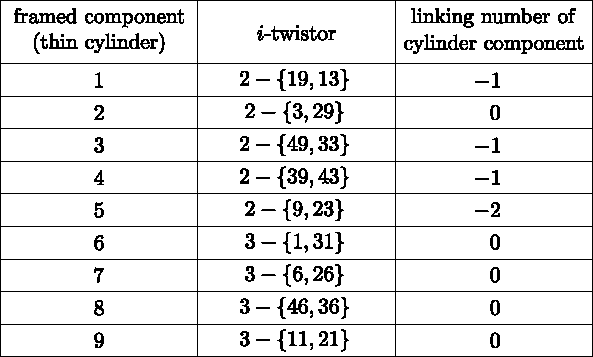
\includegraphics[width=5.8cm]{A.figs/U2.pdf}
\end{center}
\end{figure}


\section*{Appendix B: all figures for the $r_5^{24}$-example. This produces
an overview of the data structure and their interrelations illustrating the general case
of the algorithm}

In the following figures, the notation
% $\nabla_{v,1}$ denotes the PL3-face dual of the vertex $v$ in $E\mathcal{H}_1^\star$.
 $\nabla_{v,i+1}$, $i\geq1$, denotes the PL3-face dual of the
vertex $v$ of the input gem obtained after the $i$-th $bp$-move is performed. If after the $i$-th
$bp$-move $\nabla_{v,i}$ does not change, then $\nabla_{v,i+1}=\nabla_{v,i}$. When there is a change,
it is an $\epsilon$-change.


%-----------------------------------
\begin{figure}[!htb]
\begin{center}
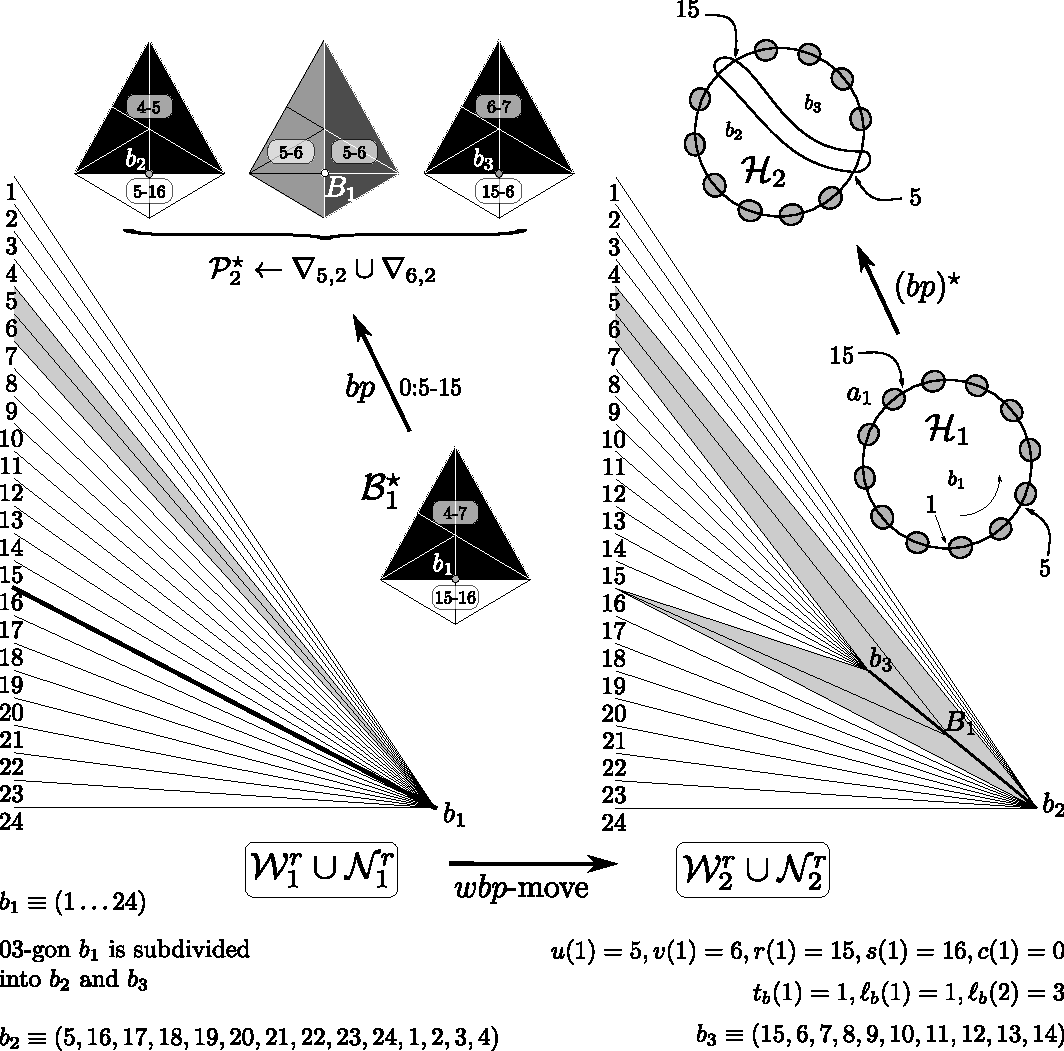
\includegraphics[width=15cm]{A.figs/bpandwinglist01.pdf} \\
\caption{\sf 
$\mathcal{H}^\star_{2} \leftarrow \mathcal{H}^\star_1 
\cup (\mathcal{P}_{2}^\star \backslash \mathcal{B}_1^\star)$. 
Pillow $\mathcal{P}_{2}^\star \leftarrow 
\nabla_{5,12}\cup \nabla_{6,12}$
($r^{24}_5$-example).}
\label{fig:winglist01}
\end{center}
\end{figure}
%-----------------------------------

%-----------------------------------
\begin{figure}
\begin{center}
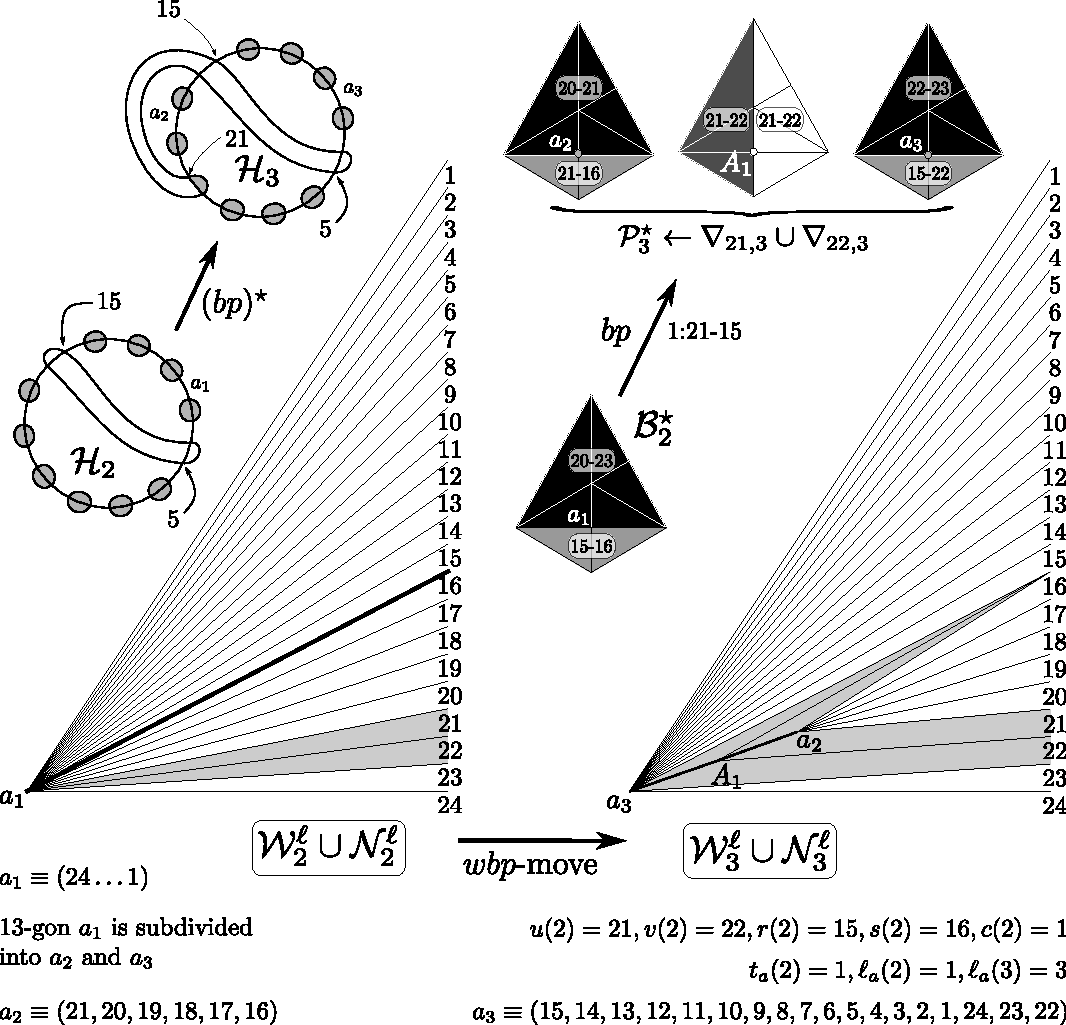
\includegraphics[width=15cm]{A.figs/bpandwinglist02.pdf} \\
\caption{\sf 
$\mathcal{H}^\star_{3} \leftarrow \mathcal{H}^\star_2 
\cup (\mathcal{P}_{3}^\star \backslash \mathcal{B}_2^\star)$. 
Pillow $\mathcal{P}_{3}^\star \leftarrow 
\nabla_{21,12}\cup \nabla_{22,12}$
($r^{24}_5$-example).}
\label{fig:winglist02}
\end{center}
\end{figure}
%-----------------------------------

%-----------------------------------
\begin{figure}
\begin{center}
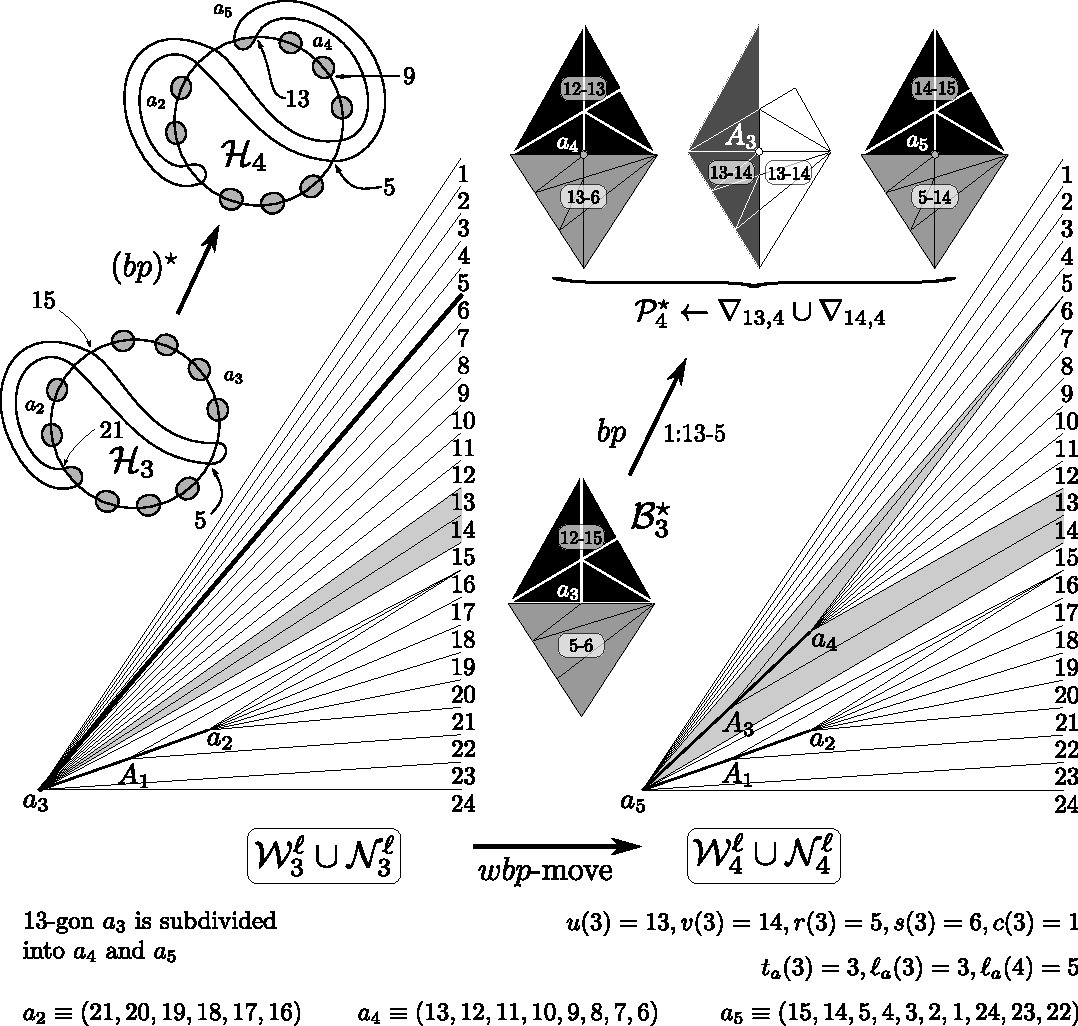
\includegraphics[width=15cm]{A.figs/bpandwinglist03.pdf} \\
\caption{\sf 
$\mathcal{H}^\star_{4} \leftarrow \mathcal{H}^\star_3 
\cup (\mathcal{P}_{4}^\star \backslash \mathcal{B}_3^\star)$. 
Pillow $\mathcal{P}_{4}^\star \leftarrow 
\nabla_{13,12}\cup \nabla_{14,12}$
($r^{24}_5$-example).}
\label{fig:winglist03}
\end{center}
\end{figure}
%-----------------------------------

%-----------------------------------
\begin{figure}
\begin{center}
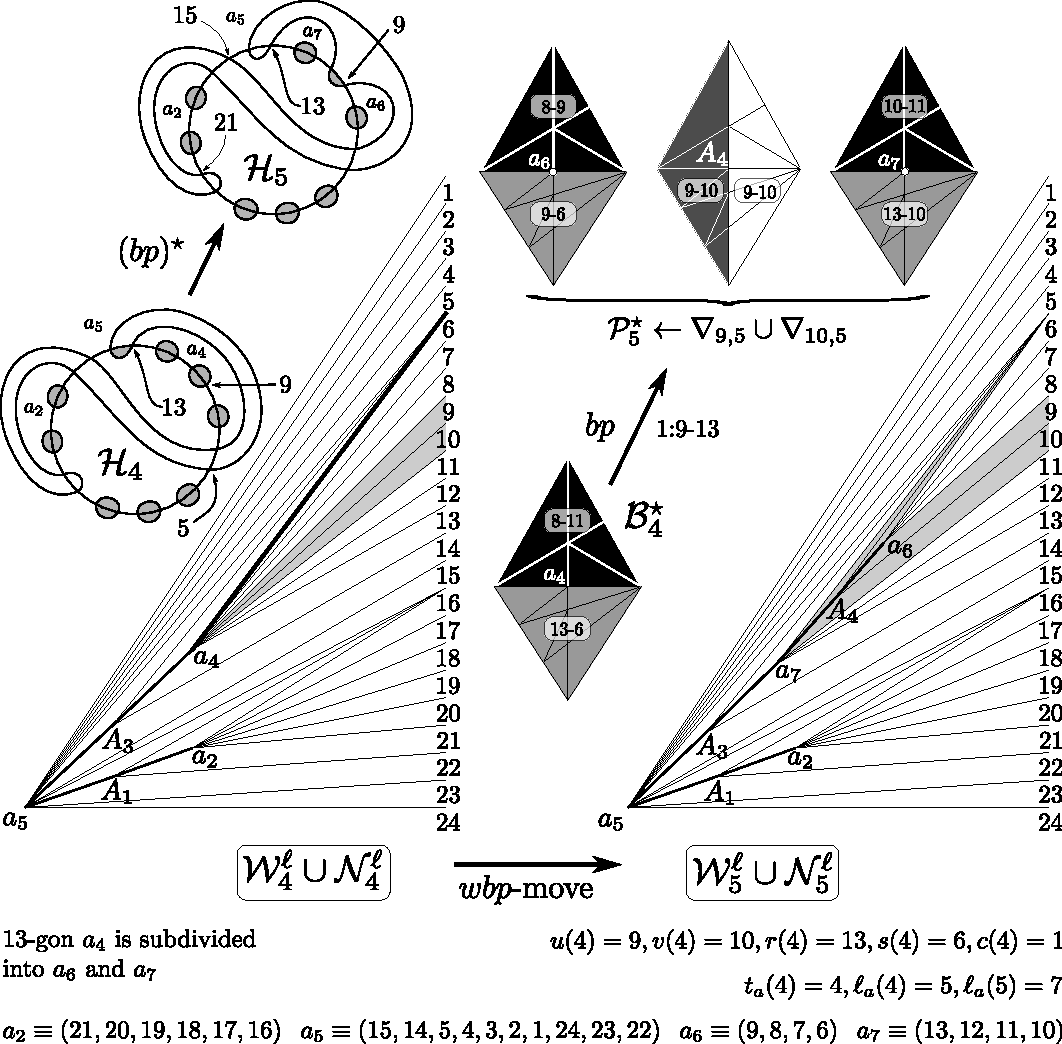
\includegraphics[width=15cm]{A.figs/bpandwinglist04.pdf} \\
\caption{\sf 
$\mathcal{H}^\star_{5} \leftarrow \mathcal{H}^\star_4 
\cup (\mathcal{P}_{5}^\star \backslash \mathcal{B}_4^\star)$. 
Pillow $\mathcal{P}_{5}^\star \leftarrow 
\nabla_{9,12}\cup \nabla_{10,12}$
($r^{24}_5$-example).}
\label{fig:winglist04}
\end{center}
\end{figure}
%-----------------------------------

%-----------------------------------
\begin{figure}
\begin{center}
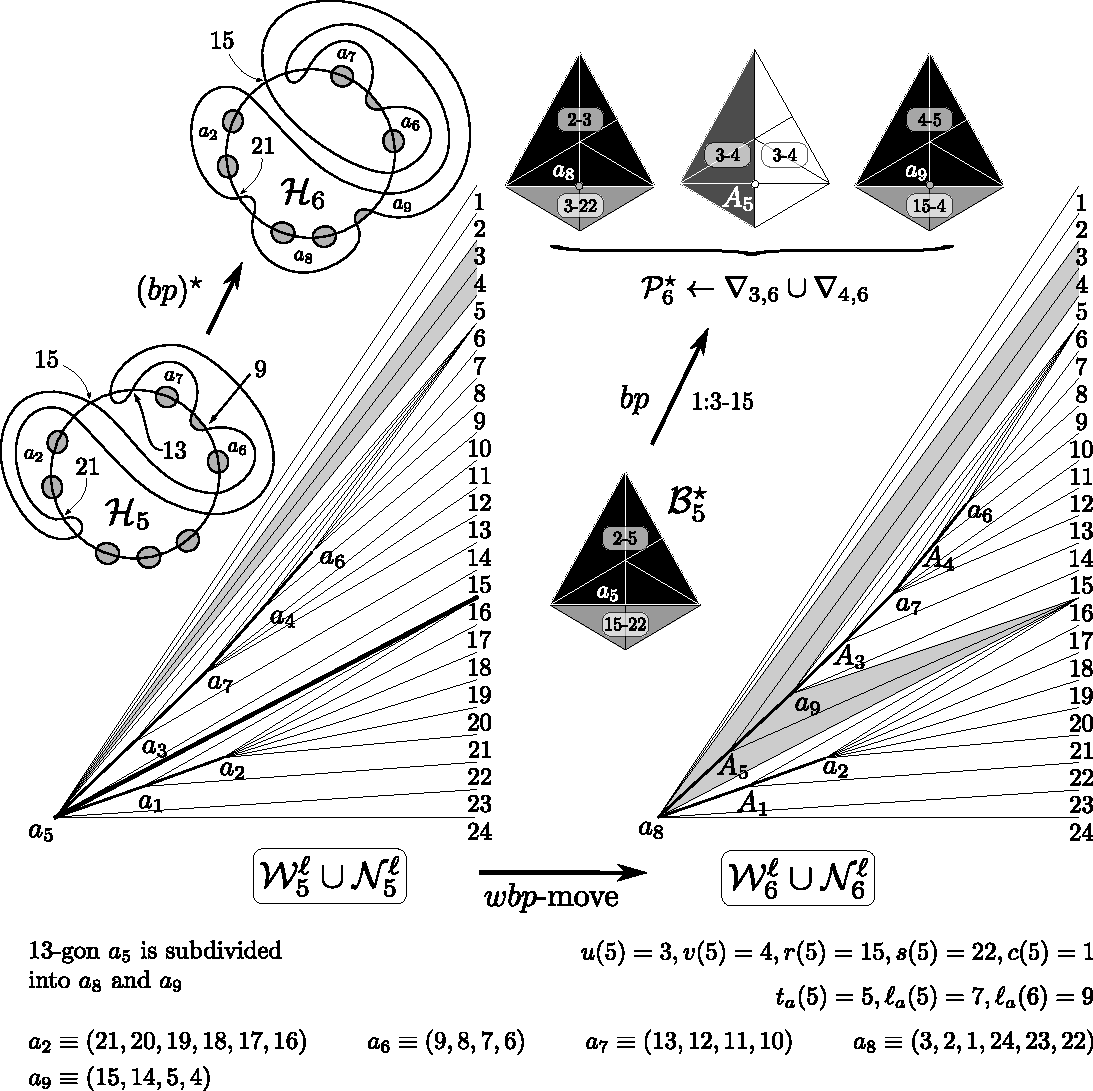
\includegraphics[width=15cm]{A.figs/bpandwinglist05.pdf} \\
\caption{\sf 
$\mathcal{H}^\star_{6} \leftarrow \mathcal{H}^\star_5 
\cup (\mathcal{P}_{6}^\star \backslash \mathcal{B}_5^\star)$. 
Pillow $\mathcal{P}_{6}^\star \leftarrow 
\nabla_{3,12}\cup \nabla_{4,12}$
($r^{24}_5$-example).}
\label{fig:winglist05}
\end{center}
\end{figure}
%-----------------------------------

%-----------------------------------
\begin{figure}
\begin{center}
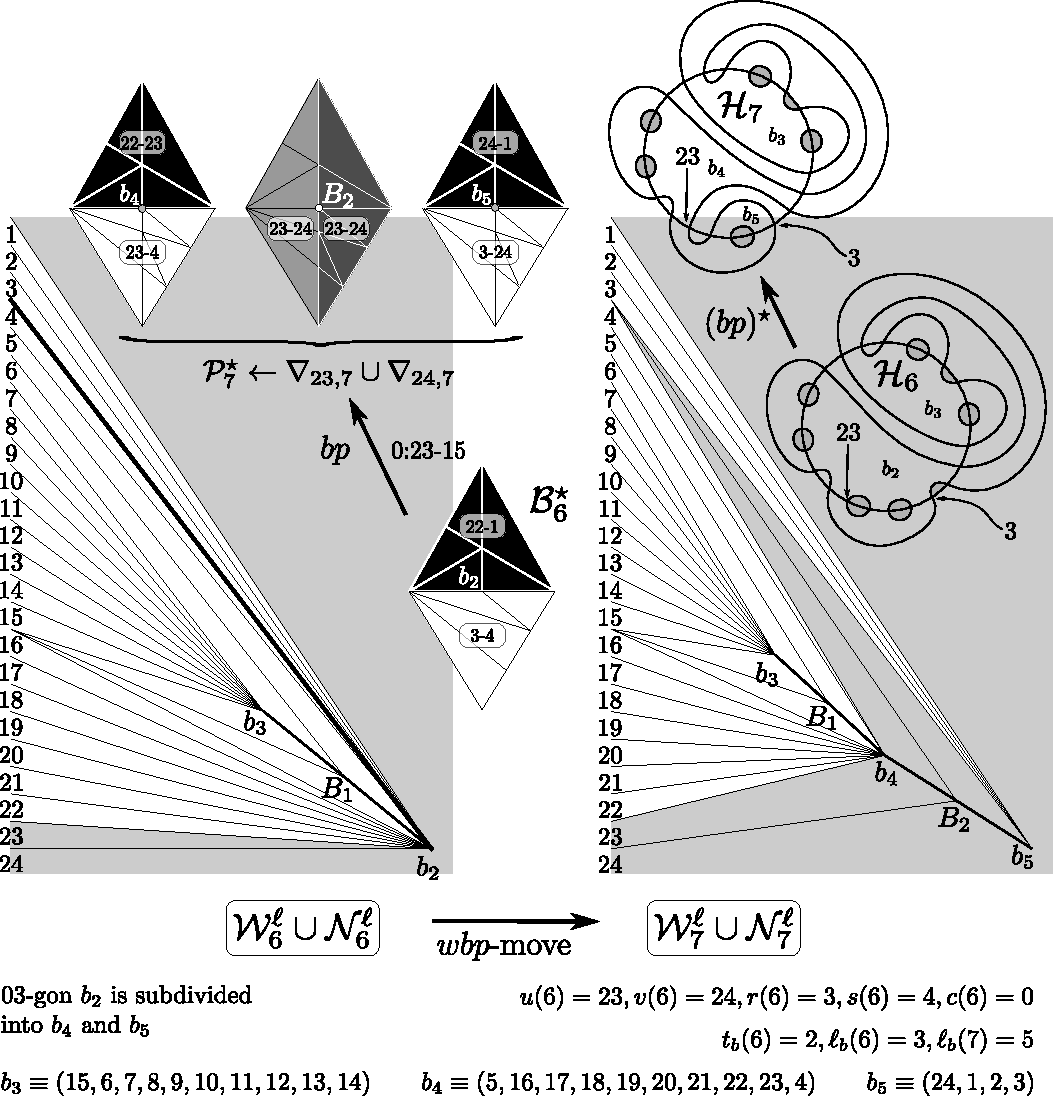
\includegraphics[width=15cm]{A.figs/bpandwinglist06.pdf} \\
\caption{\sf 
$\mathcal{H}^\star_{7} \leftarrow \mathcal{H}^\star_6 
\cup (\mathcal{P}_{7}^\star \backslash \mathcal{B}_6^\star)$. 
Pillow $\mathcal{P}_{7}^\star \leftarrow 
\nabla_{23,12}\cup \nabla_{24,12}$
($r^{24}_5$-example).}
\label{fig:winglist06}
\end{center}
\end{figure}
%-----------------------------------


%-----------------------------------
\begin{figure}
\begin{center}
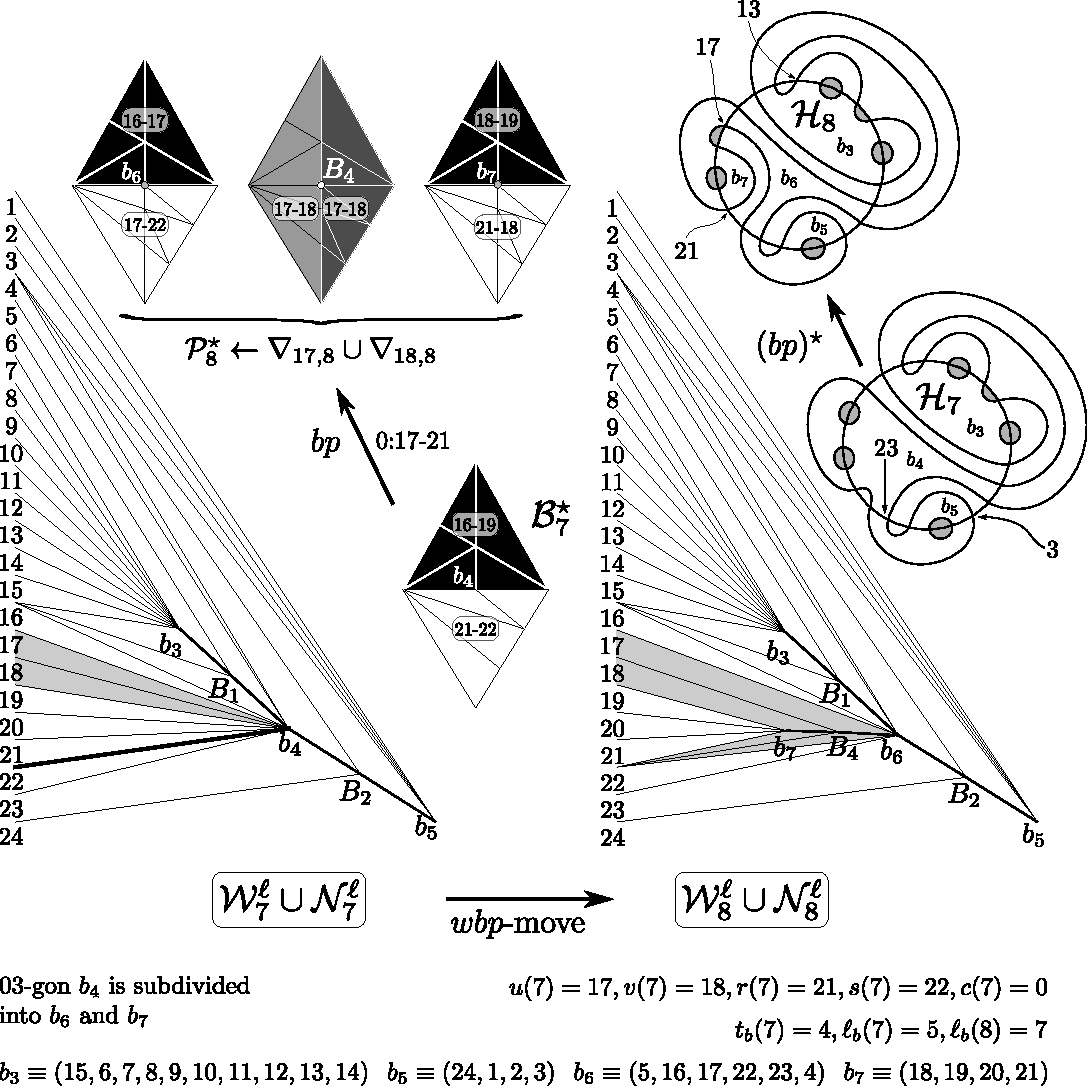
\includegraphics[width=15cm]{A.figs/bpandwinglist07.pdf} \\
\caption{\sf 
$\mathcal{H}^\star_{8} \leftarrow \mathcal{H}^\star_7 
\cup (\mathcal{P}_{8}^\star \backslash \mathcal{B}_7^\star)$. 
Pillow $\mathcal{P}_{8}^\star \leftarrow 
\nabla_{17,12}\cup \nabla_{18,12}$
($r^{24}_5$-example).}
\label{fig:winglist07}
\end{center}
\end{figure}
%-----------------------------------

%-----------------------------------
\begin{figure}
\begin{center}
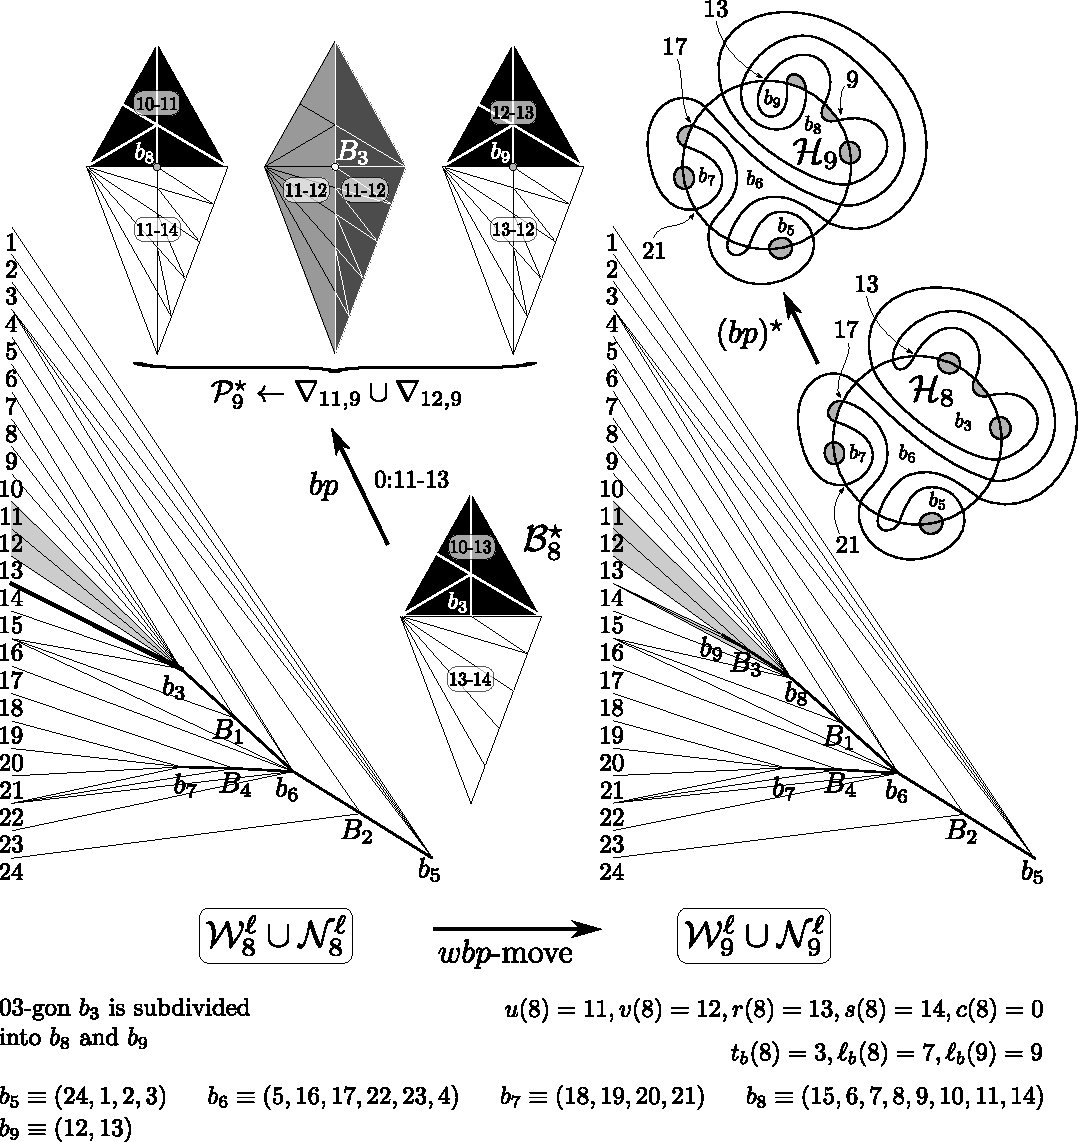
\includegraphics[width=15cm]{A.figs/bpandwinglist08.pdf} \\
\caption{\sf 
$\mathcal{H}^\star_{9} \leftarrow \mathcal{H}^\star_8 
\cup (\mathcal{P}_{9}^\star \backslash \mathcal{B}_8^\star)$. 
Pillow $\mathcal{P}_{9}^\star \leftarrow 
\nabla_{11,12}\cup \nabla_{12,12}$
($r^{24}_5$-example).}
\label{fig:winglist08}
\end{center}
\end{figure}
%-----------------------------------

%-----------------------------------
\begin{figure}
\begin{center}
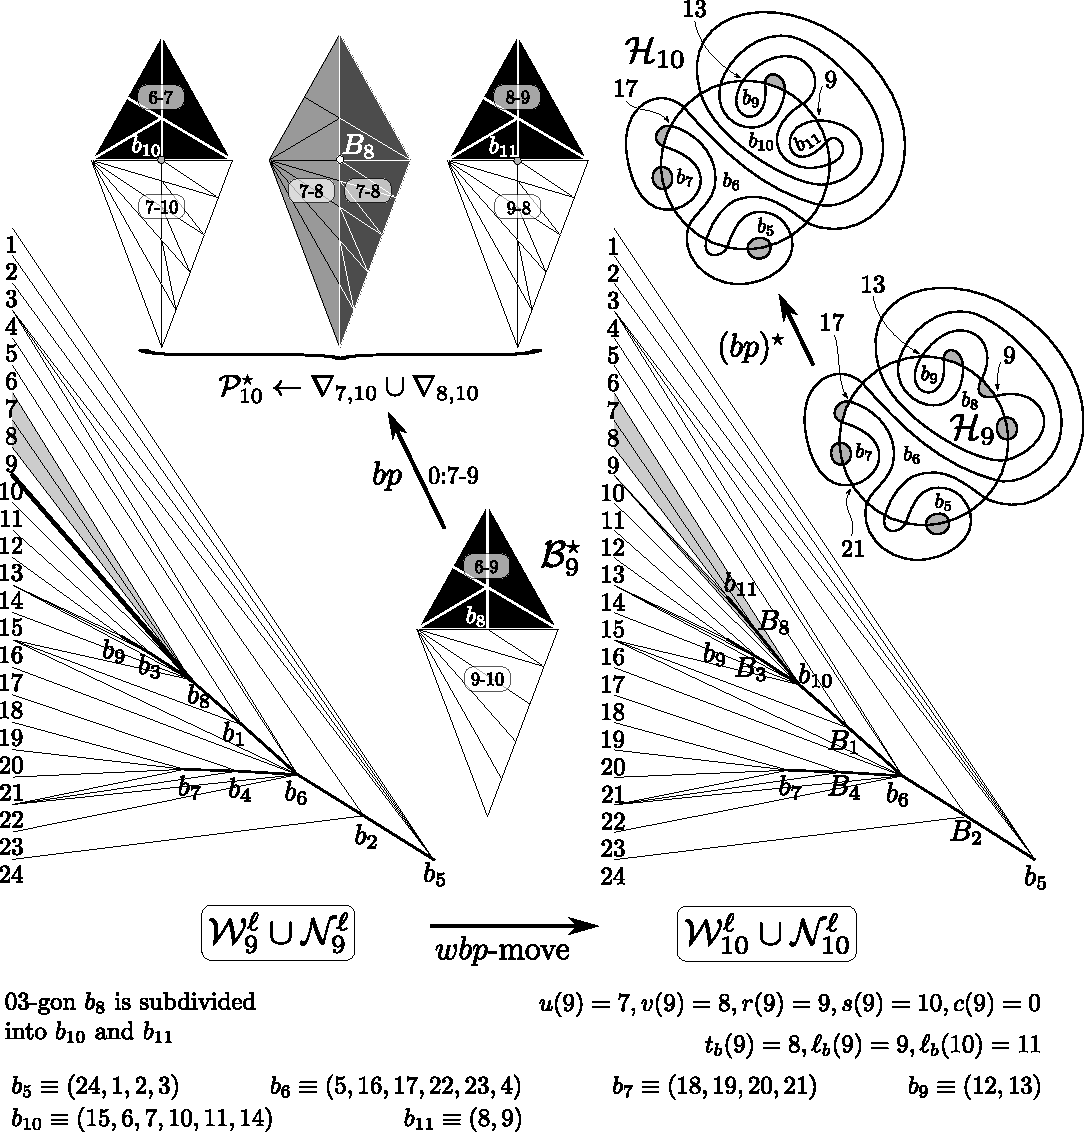
\includegraphics[width=15cm]{A.figs/bpandwinglist09.pdf} \\
\caption{\sf 
$\mathcal{H}^\star_{10} \leftarrow \mathcal{H}^\star_9 
\cup (\mathcal{P}_{10}^\star \backslash \mathcal{B}_9^\star)$. 
Pillow $\mathcal{P}_{10}^\star \leftarrow 
\nabla_{7,12}\cup \nabla_{8,12}$
($r^{24}_5$-example).}
\label{fig:winglist09}
\end{center}
\end{figure}
%-----------------------------------

%-----------------------------------
\begin{figure}
\begin{center}
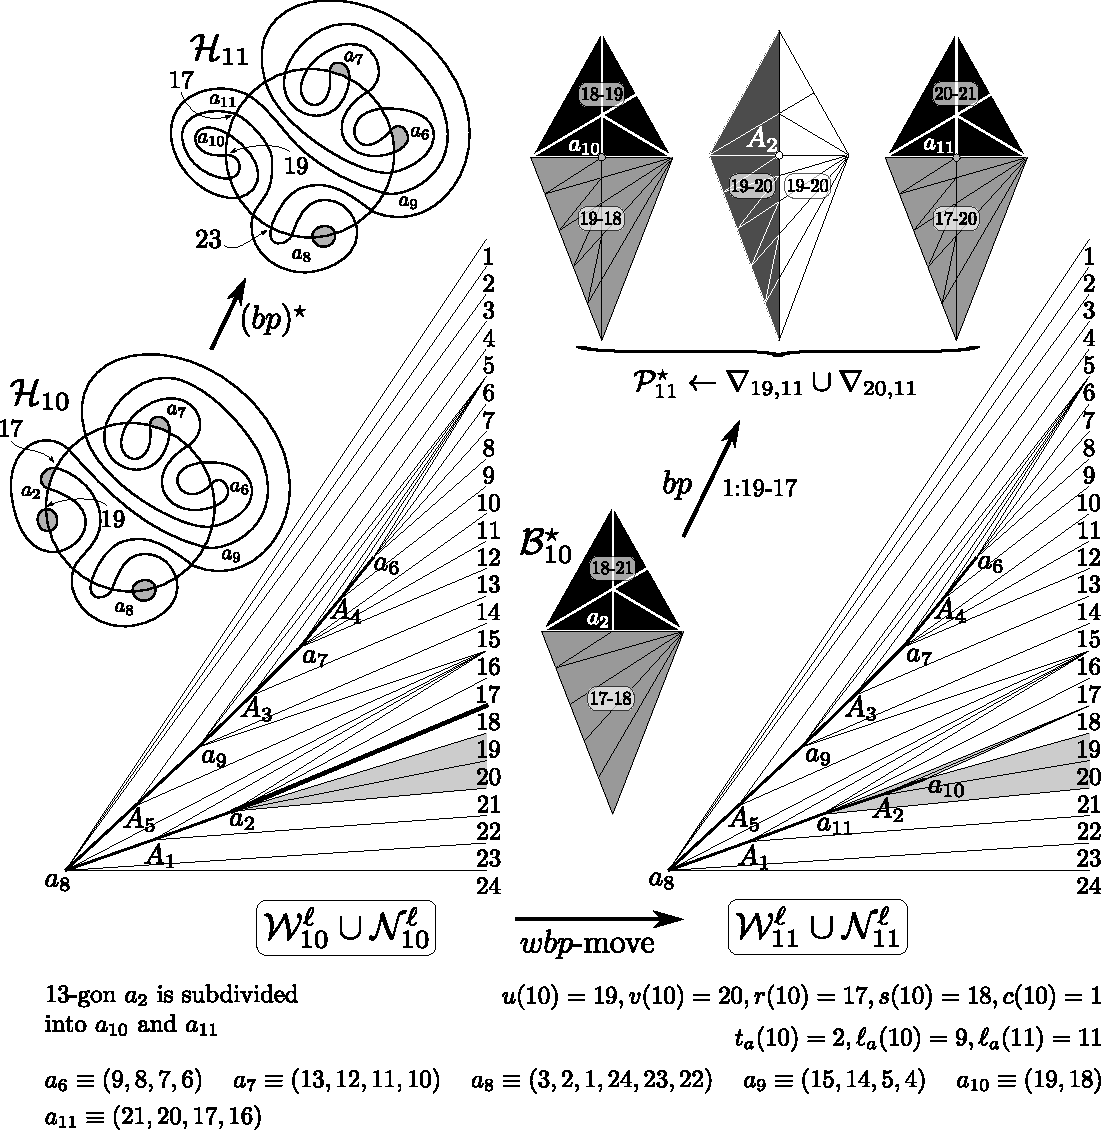
\includegraphics[width=15cm]{A.figs/bpandwinglist10.pdf} \\
\caption{\sf 
$\mathcal{H}^\star_{11} \leftarrow \mathcal{H}^\star_{10}
\cup (\mathcal{P}_{11}^\star \backslash \mathcal{B}_{10}^\star)$.
Pillow $\mathcal{P}_{11}^\star \leftarrow 
\nabla_{19,12}\cup \nabla_{20,12}$
($r^{24}_5$-example).}
\label{fig:winglist10}
\end{center}
\end{figure}
%-----------------------------------

%-----------------------------------
\begin{figure}
\begin{center}
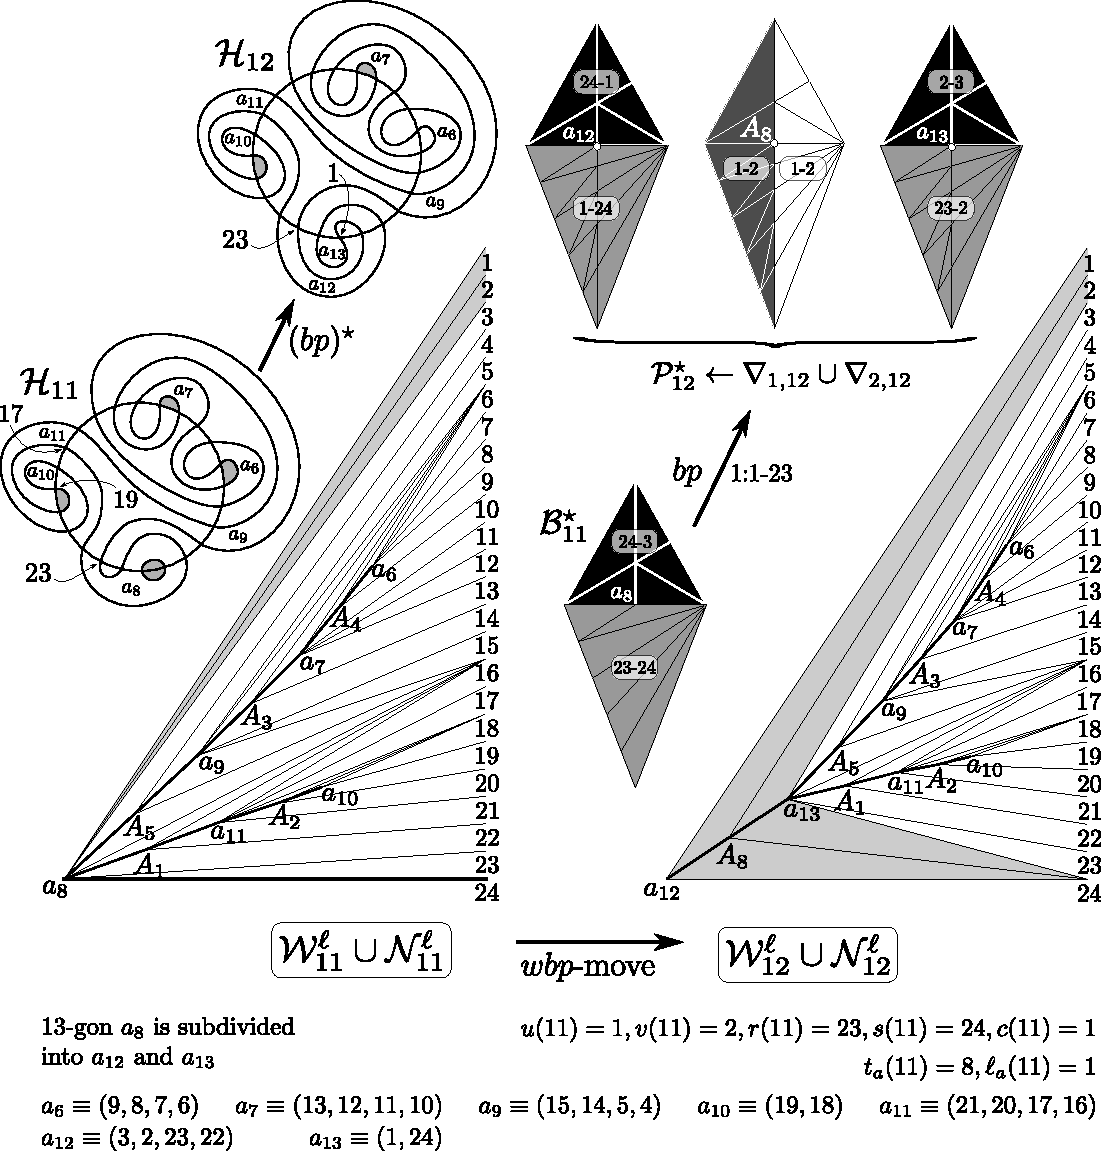
\includegraphics[width=15cm]{A.figs/bpandwinglist11.pdf} \\
\caption{\sf 
$\mathcal{H}^\star_{12} \leftarrow \mathcal{H}^\star_{11} 
\cup (\mathcal{P}_{12}^\star \backslash \mathcal{B}_{11}^\star)$. 
Pillow $\mathcal{P}_{12}^\star \leftarrow \nabla_{1,12}\cup \nabla_{2,12}$
($r^{24}_5$-example).}
\label{fig:winglist11}
\end{center}
\end{figure}
%-----------------------------------

%-----------------------------------
%\begin{figure}
%\begin{center}
%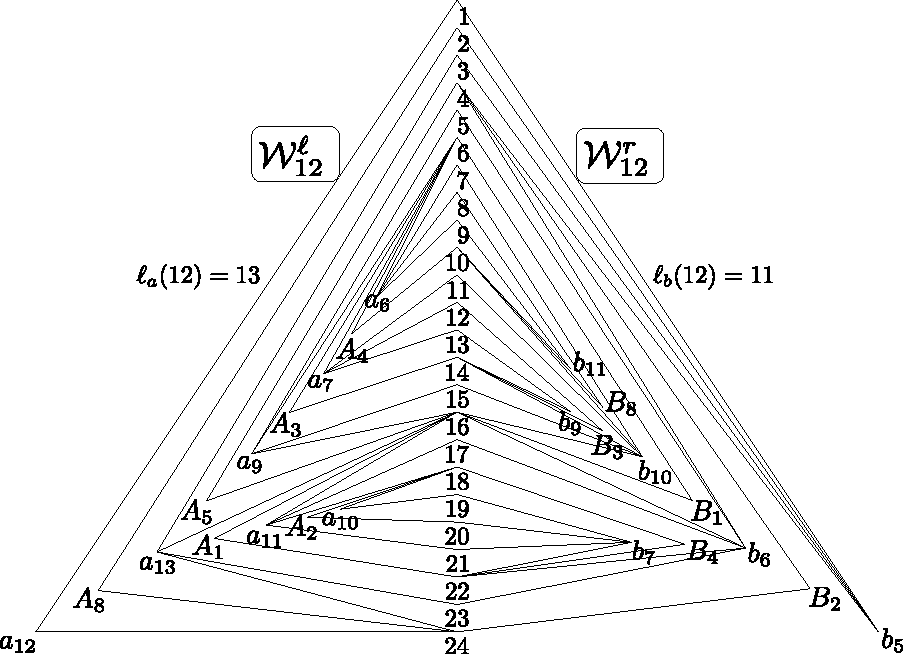
\includegraphics[width=15cm]{A.figs/bpandwinglist12.pdf} \\
%\caption{\sf 
%$\mathcal{H}^\star_{12} \leftarrow \mathcal{H}^\star_{11} 
%\cup (\mathcal{P}_{12}^\star \backslash \mathcal{B}_{11}^\star)$ 
%and wings (without nervures) of $\mathcal{H}^\star_{12}$
%($r^{24}_5$-example).}
%\label{fig:winglist12}
%\end{center}
%\end{figure}



%-----------------------------------
%\bibliographystyle{plain}
%\bibliographystyle{is-alpha}
%\addcontentsline{toc}{bibliografia}{\MakeTextUppercase{Refer�ncias Bibliogr�ficas}}
%\bibliography{d:/slsl\3.DadosSostenes.35.ArtigosLivros.bibtexGoogleScholar/bibtexIndex.bib} % bib file is slsl.bib
%\bibliography{~/home/ricardo/Dropbox/35.ArtigosLivros.bibtexGoogleScholar/bibtexIndex.bib}
%\bibliography{bibtexIndex.bib}
%\bibliography{slsl}

% \vspace{10mm}
% \begin{center}
% 
% 
% \hspace{7mm}
% \begin{tabular}{l}
%    S\'ostenes L. Lins\\
%    Centro de Inform\'atica, UFPE \\
%    Recife--PE \\
%    Brazil\\
%    sostenes@cin.ufpe.br
% \end{tabular}
% \hspace{20mm}
% \begin{tabular}{l}
%    Ricardo N. Machado\\
%    N�cleo de Forma��o de Docentes, UFPE\\
%    Caruaru--PE \\
%    Brazil\\
%    ricardonmachado@gmail.com
% \end{tabular}
% 
% \end{center}


%\end{document}







\begin{abstract}
Let be given a {\em colored 3-pseudo-triangulation} $\mathcal{H}^\star$ with $n$ tetrahedra.
Colored means that each tetrahedron have vertices 
distinctively colored 0,1,2,3.
In a {\em pseudo} 3-triangulation the intersection of simplices might be subsets of simplices
of smaller dimensions, instead of singletons of such faces, 
as for true triangulations. If $\mathcal{H}^\star$ is the dual of a $J^2$-gem 
(shortly to be defined in the Introduction),
then we show that the induced 3-manifold $|\mathcal{H}^\star|$ is $\mathbb{S}^3$ and we make available an $O(n^2$)-algorithm to produce a
PL-embedding (\cite{rourke1982introduction}) of $\mathcal{H}^\star$ into $\mathbb{S}^3$.
This is rather surprising because such PL-embeddings are often of exponential size.
This work is the first step towards obtaining, via an $O(n^ 2)$-algorithm,
a framed link presentation inducing the same closed orientable 3-manifold
as the one given by a colored pseudo-triangulation. 
% A {\em $J^ 2$-gem} is a 4-regular, 4-edge-colored planar graph $\mathcal{H}$ obtained from the
% intersection pattern of two Jordan curves $X$ and $Y$ with $2n$ transversal
% crossings.
% These crossings define consecutive segments of $X$ alternatively 
% inside $Y$ and outside $Y$. Color the first type 2 and the second type 3.
% The crossings also define consecutive segments of $Y$ alternatively 
% inside $X$ and outside $X$. Color the first type 0 and the second type 1.
% This defines a 4-regular 4-edge-colored graph $\mathcal{H}$ where the vertices are the crossings
% and the edges are the colored colored segments.
% Let $\mathcal{H}^ \star$ be the 3-dimensional abstract 3-complex formed by taking a set of 
% vertex colored tetrahedra in 1--1 correspondence with $V(\mathcal{H})$ so that each tetrahedra
% has vertices of colors 0,1,2,3. For each $i$-colored edge of $\mathcal{H}$ with ends $u$ and $v$
% paste the corresponding tetrahedra $\nabla_u$ and $\nabla_v$ so as to paste the two triangular
% faces that do not contain a vertex of color $i$ in such a way as to
% to match vertices of the other three colors. 
% We show that the topological space 
% $|\mathcal{H}^\star|$ induced by $\mathcal{H}^\star$ is $\mathbb{S}^ 3$. Moreover we describe an $O(n^2)$-algorithm
% to make available a PL-embedding (\cite{rourke1982introduction}) of $\mathcal{H}^\star$ 
% into $\mathbb{S}^3$. We get explicit coordinates in $\mathbb{S}^ 3$ for the 0-simplices and
% the p-simplices $(p \in \{1,2,3\}$) are linear simplices in the spherical geometry.
Previous work on this topic appear in
\cite{linsmachadoA2012}, \cite{linsmachadoB2012} and \cite{linsmachadoC2012}.
However, the exposition and the new proofs of this paper are meant to be entirely self-contained.

\end{abstract}


\section{Introduction}
\subsection{$J^2$-gems}
A {\em $J^ 2$-gem} is a 4-regular, 4-edge-colored planar graph $\mathcal{H}$ obtained from the
intersection pattern of two Jordan curves $X$ and $Y$ with $2n$ transversal
crossings.
These crossings define consecutive segments of $X$ alternatively 
inside $Y$ and outside $Y$. Color the first type 2 and the second type 3.
The crossings also define consecutive segments of $Y$ alternatively 
inside $X$ and outside $X$. Color the first type 0 and the second type 1.
This defines a 4-regular 4-edge-colored graph $\mathcal{H}$ where the vertices are the crossings
and the edges are the colored colored segments.
Let $\mathcal{H}^\star$ be the 3-dimensional abstract 3-complex formed by taking a set of 
vertex colored tetrahedra in 1--1 correspondence with the set of vertices of $\mathcal{H}$,
$V(\mathcal{H})$, so that each tetrahedra
has vertices of colors 0,1,2,3. This vertex coloring induces a face coloring of the 
triangular faces of the tetrahedron: color $i$ the face opposite to the vertex colored $i$.
For each $i$-colored edge of $\mathcal{H}$ with ends $u$ and $v$
paste the corresponding tetrahedra $\nabla_u$ and $\nabla_v$ so as to paste the two triangular
faces that do not contain a vertex of color $i$ in such a way as to
to match vertices of the other three colors. 
We show that the topological space 
$|K|$ induced by $\mathcal{H}^\star$ is $\mathbb{S}^ 3$. Moreover we describe an $O(n^2)$-algorithm
to make available a PL-embedding (\cite{rourke1982introduction}) of $\mathcal{H}^\star$ 
into $\mathbb{S}^3$. We get explicit coordinates in $\mathbb{S}^ 3$ for the 0-simplices and
the p-simplices $(p \in \{1,2,3\}$) are linear simplices in the spherical geometry.


\subsection{Gems and their duals}
A {\em (3+1)-graph} \index{(3+1)-graph} $\mathcal{H}$ is a connected regular graph of degree 4 where 
to each vertex there are four incident differently colored edges in the color 
set $\{0,1,2,3\}$.
\index{residue}
For $I \subseteq \{0,1,2,3\}$, an {\em $I$-residue} is a component of the subgraph 
induced by the $I$-colored edges. Denote by $v(\mathcal{H})$ the number of
$0$-residues (vertices) of $\mathcal{H}$. For $0\le i < j\le3$, an $\{i,j\}$-residue is also 
called an {\em $ij$-gon} or an $i$- and $j$-colored {\em bigon} (it is an even polygon, where the edges are 
alternatively colored $i$ and $j$). Denote by $b(\mathcal{H})$ the total number of $ij$-gons 
for $0\le i < j\le3$. Denote by $t(\mathcal{H})$ the total number of 
$\overline{i}$-residues for $0\le i\le 3$, where $\overline{i}$ 
means complement of $\{i\}$ in $\{0,1,2,3\}$.

We briefly recall the definition of gems taken from \cite{lins1995gca}.
A {\em $3$-gem} \index{3-gem} is a $(3+1)$-graph $\mathcal{H}$
satisfying $v(\mathcal{H})+t(\mathcal{H})=b(\mathcal{H})$. This relation is equivalent to having the vertices, 
edges and bigons 
restricted to any $\{i,j,k\}$-residue inducing a plane graph where the 
faces are bounded by the 
bigons. Therefore we can embed each such $\{i,j,k\}$-residue into a sphere 
$\mathbb{S}^2$. We consider
the ball bounded this $\mathbb{S}^2$ as induced by the  $\{i,j,k\}$-residue. For this reason
an $\{i,j,k\}$-residue in a 3-gem, $i<j<k$, is also called a \index{triball} {\em triball}.
An $ij$-gon appears once in the boundary of triball $\{i,j,k\}$ and once in the boundary
of triball $\{i,j,h\}$. By pasting the triballs along disks bounded by all 
the pairs of $ij$-gons, $\{i,j\} \subset \{0,1,2,3\}$ of a gem $\mathcal{H}$,
we obtain a closed 3-manifold denoted by $|\mathcal{H}|$. 
This general construction is dual to the one 
exemplified in the abstract and produces any closed 3-manifold. 
The manifold is orientable if and only if 
$\mathcal{H}$ is bipartite, \cite{lins1985graph}. A {\em crystallization} is a
gem which remains connected after deleting all the edges of any given color, that is,
it has one $\{i,j,k\}$-residue for each trio of colors $\{i,j,k\} \subset \{0,1,2,3\}$.

Let $\mathcal{H}^\star$ be the dual of a gem $\mathcal{H}$.
An $\overline{i}$-residue of $\mathcal{H}$ corresponds in $\mathcal{H}^\star$ to a $0$-simplex of $\mathcal{H}^\star$. Most 0-simplices of $\mathcal{H}^\star$
do not correspond to $\overline{i}$-residues of $\mathcal{H}$.
An $ij$-gon of a gem $\mathcal{H}$ corresponds in $\mathcal{H}^\star$ to a {\em PL1-face} formed by a sequence of
1-simplices of $\mathcal{H}^\star$; this PL1-face is the intersection of two PL2-faces of colors $i$ and $j$; their
two bounding $0$-simplices correspond to an $\overline{h}$- and to a $\overline{k}$-residue, where
$\{h,i,j,k\}=\{0,1,2,3\}$.
An $i$-colored edge of $\mathcal{H}$ corresponds to a {\em PL2-face} 
which is a 2-disk triangulated by a subset of $i$-colored 2-simplices of $\mathcal{H}^\star$. Finally to a vertex of $\mathcal{H}$, 
it corresponds a {\em PL3-face} of $\mathcal{H}^\star$ which is a 3-ball formed by a subset of 3-simplices of $\mathcal{H}^\star$.

\begin{proposition}
\label{prop:j2shere}
The $3$-manifold induced by a $J^2$-gem $\mathcal{H}$ is $\mathbb{S}^3$.
\end{proposition}
\begin{proof}
Removing from $\mathcal{H}$ all the edges of a given color still yields a connected graph
which a plane graph and they come embedded so that the faces are the 2-residues.
So $\mathcal{H}$ has four 3-residues, one of each type. 
Denote by $b_{ij}$ the number of $ij$-gons of $\mathcal{H}$.
Each one of these residues are planar graphs
having $v=2n$ vertices, $3v/2$ edges and $b_{12}+b_{13}+b_{23}$, 
$b_{02}+b_{03}+b_{23}$, $b_{01}+b_{13}+b_{03}$ and  $b_{12}+b_{01}+b_{02}$ faces
for, respectively, the $\overline{0}$-, $\overline{1}$-, $\overline{2}$-, 
$\overline{3}$-residue. Adding the four formulas for the Euler characteristic of the sphere
imply that $v(\mathcal{H})+4=b(\mathcal{H})$. Therefore, $\mathcal{H}$ is a crystallization having one $0i$-gon and
one $jk$-gon. This implies that the fundamental group of the induced manifold is trivial:
as proved in \cite{lins1988fundamental}, the fundamental group of the space induced by a crystallization
is generated by $b_{0i}-1$ generators, and in our case this number is 0.
Since Poincar� Conjecture is now proved, we are done. 
However, we can avoid using this fact and, as a bonus, obtaining the validity
of the next corollary, which is used in the sequel.

Assume that $\mathcal{H}$ is a $J^2$-gem which does not induce $\mathbb{S}^3$ and has the smallest possible
number of vertices satisfying these assumptions. By planarity we must have a pair of edges of
$\mathcal{H}$ having the same ends $\{p,q\}$. Consider the graph $\mathcal{H} fus \{p,q\}$ obtained from
$\mathcal{H}$ by removing the vertices $p$, $q$ and the 2 edges linking them as well as welding the 2
pairs of pendant edges along edges of the same color. In \cite{lins1985simple} S. Lins proves that
if $\mathcal{H}$ is a gem, $\mathcal{H}'=\mathcal{H} fus \{p,q\}$ is also a gem and that two exclusive 
relations hold regarding $|\mathcal{H}|$ and $ |\mathcal{H}'|$, their induced 3-manifolds:
either $|\mathcal{H}| = |\mathcal{H}'|$ in the case that $\{p,q\}$ induces a 2-dipole
or else  $|\mathcal{H}| = |\mathcal{H}'| \# (\mathbb{S}^2\times \mathbb{S}^1)$. Since
$\mathcal{H}'$ is a $J^2$-gem, by our minimality hypothesis on $\mathcal{H}$
the valid alternative is the second. But this
is a contradiction: the fundamental group of $|\mathcal{H}|$ would not be trivial, 
because of the summand $\mathbb{S}^2\times \mathbb{S}^1$. 
\end{proof}


\subsection{Dipoles, pillows and balloons} 

Suppose there are $m$ edges linking vertices $x$ and $y$ of a gem, $m \in \{1,2,3\}$.
We say that $\{u,v\}$ is an {\em $m$-dipole} if removing all edges in the colors of the ones linking $x$ to $y$,
these vertices are in distinct components of the graph induced by the edges in the complementary
set of colors. To {\em cancel the dipole} means deleting the subgraph induced by $\{u,v\}$ and identify pairs 
of the hanging edges along the same remaining color. To {\em create the dipole} is the inverse operation.
It is simple to prove that the manifold of a gem is invariant under dipole cancellation or creation.
Even though is not relevant for the present work state the foundational result on gems: two $3$-manifolds
are homeomorphic if and only if any two gems inducing it are linked by a finite number of
cancellations and creations of dipoles, \cite{ferri1982crystallisation, lins2006blobs}.

The dual of a $2$-dipole $\{u,v\}$, with internal colors $i,j$ is named a {\em pillow}. 
It consistes of two PL3-faces $\nabla_u$ and $\nabla_v$ sharing two PL2-faces colored $i$ and $j$.
The {\em thickening of a 2-dipole into a 3-dipole} is defined as follows. Let
$i,j$ be the two colors internal to 2-dipole $\{u,v\}$ and $k$ a third color.
Let $a$ be the $k$-neighboor of $x$ and $b$ be the $k$-neighboor of $y$. Remove
edges $[a,x]$ and $[b,y]$ and put back $k$-edges $[u,v]$ and $[r,s]$. This completes
the thickening. It is simple to prove that the thickening in a gem produces a gem. 
We must be carefull because the inverse blind inverse operation {\em thinning a 3-dipole} 
not always produces a gem. The catch is that the result of the thinning perhaps is not a 2-dipole.
In this sense the thinning move is not local: we must make sure that the result is a 2-dipole.
To the data needed in thinning a 3-dipole $\{u,v\}$ with internal colors $\{i,j,k\}$ 
we must add the $k$-edge $[r,s]$. Note that the $k$-edges $[u,v]$ and $[r,s]$ are in the same $hk$-gon,
where $h$ is the fourth color. Denote by $\Delta_{rs}$ the dual of $[r,s]$.
Let $\nabla_u \cup \nabla v \cup \Delta_{rs}$ be called a {\em balloon}. 
Note that it consists of 2 PL3-faces $\nabla_u$ and $\nabla_v$ sharing three PL2-faces 
in colors $\{i,j,k\}$ together
with a $k$-colored PL2-face whose intersection with  $\nabla_u \cup \nabla_v$ is 
a PL1-face corresponding to the dual of the $hk$-gon, where $h$ is the fourth color.
Let $\nabla_u \cup \nabla_v$ be the {\em balloon's head} and let $\Delta_{rs}$
be the {\em balloon's tail}.


\subsection{The Strategy for finding the $O(n^2)$-algorithm}
We want to find a PL-embedding for the dual $\mathcal{H}^\star$ of a $J^2$-gem $\mathcal{H}$ 
into $\mathbb{S}^3$. To this end we remove one PL3-face of $\mathcal{H}^\star$ 
(one vertex of $\mathcal{H}$) and find
a PL-embedding in $\mathbb{R}^3$  forming a a PL-triangulated tetrahedron. 
After we use the inverse of a stereographic projection with center
in the exterior of the triangulated tetrahedron. In this way we recover in $\mathbb{S}^3$
the missing PL3-face.

In this work we describe the PL-embedded PL3-faces of $\mathcal{H}^\star$ 
into $\mathbb{R}^3$ by making it geometrically clear that its boundary
is a set of 4 PL2-faces, one of each color, forming an embedded $\mathbb{S}^2$ whose interior is
disjoint from the interior of 
$\mathbb{S}^2$'s corresponding to others PL3-faces. Thus, for our purposes
it will be only necessary to embed the 2-skeleton of $\mathcal{H}^\star$.

A direct approach to find the PL-embedding of the dual of a general $J^2$-gem with $2n$ vertices,
seems very hard. Therefore, we split the algorithm into 4 phases. 

In the first phase we find a sequence of $n-1$ 2-dipole thickenings into
3-dipoles not using color 3, where the new involved edge is either 0 or 1 so that the 
final gem is simply a circular arrangement 
of $n$ 3-dipoles with internal
colors $0,1,2$. Such a canonical $n$-gem is 
named a {\em bloboid} and is denoted $\mathcal{B}_n$. 
Such 3-dipoles are also named a {\em blob over a 3-colored edge}.
A $J^2B$-gem is a gem that, after cancelling blobs over $3$-colored edge becomes
a $J^2$-gem. 
This indexing decreasing sequence is easily obtainable from the
primal objects, in the case, simplifying $J^2B$-gems until the bloboid is obtained: 
$$\mathcal{H}=\mathcal{H}_{n} \mapright{2dip}{thick_1} \mathcal{H}_{n-1} \mapright{2dip}{thick_2} \ldots 
\mapright{2dip}{thick_{n-1}} \mathcal{H}_{1}=\mathcal{B}_n=\mathcal{B}.$$ 

In the second phase we first find (phase 2A) specific abstract PL-triangulations, 
for the PL2-faces for the index increasing sequence of abstract colored 2-dimensional PL-complexes.
Each of these complexes, latter, are going to be PL-embedded into $\mathbb{R}^3$ so 
that the PL2-faces are topologically 2-spheres with disjoint interior. Attaching 
3-balls bounded by these spheres we get the dual of the $J^2$-gem $\mathcal{H}$ (with a vertex
removed).
$$\mathcal{B}^\star=\mathcal{H}^\star_{1} \mapright{bp}{move_1}  \mathcal{H}^\star_{2}  
\mapright{bp}{move_{2}} \ldots
\mapright{bp}{move_{n-1}} \mathcal{H}^\star_{n}=\mathcal{H}^\star.$$ 
In parallel to the construction of the sequence $\mathcal{H}^\star_{m}$'s we also construct
(phase 2B) a sequence of {\em wings} $\mathcal{W}_{m}$'s and their {\em nervures} 
$\mathcal{N}_{m}$'s so that  
$\mathcal{S}_m=\mathcal{W}_{m} \cup \mathcal{N}_{m}$,
called {\em a strut}, is an adequate planar graph, defined recursively. 
Moreover, wings and nervures are partitioned into their {\em left} and {\em right} parts: 
$\mathcal{W}_m=\mathcal{W}'_m \cup \mathcal{W}''_m$ and
$\mathcal{N}_m=\mathcal{N}'_m \cup \mathcal{N}''_m$. The sequence of struts is
$$\mathcal{S}_1^\star=\mathcal{W}_{1} \cup \mathcal{N}_{1} 
\mapright{wbp}{move_{1}} 
\mathcal{S}_2^\star=\mathcal{W}_{2} \cup \mathcal{N}_{2} \mapright{wbp}{move_{2}} \ldots
\mapright{wbp}{move_{n-1}} 
\mathcal{S}_n^\star=\mathcal{W}_{n} \cup \mathcal{N}_{n}=
\mathcal{W} \cup \mathcal{N}=\mathcal{S}^\star.$$ 
Each wing $\mathcal{W}_m$'s corresponds to a section 
of the previous sequence $\mathcal{H}_m^\star$'s by two adequated 
fixed semi-planes $\Pi'$ and $\Pi''$.
The construction of the struts (which are planar graphs) is
recursive. Initially $\mathcal{W}_1^\star$ is a pincel of lines and $\mathcal{N}_1^\star$ 
is $\varnothing$.  Going from $\mathcal{S}^\star_{m}$
to $\mathcal{S}_{m+1}^\star$ is very simple: two new vertices and four
new edges appear, so as to maintain planarity.
% a vertex is broken into two
% and a new vertex of $\mathcal{N}_{m}^\star$ appear;
% two new edges are adjoined to $\mathcal{W}_{m}^\star$ and two new edges are adjoined to 
% $\mathcal{N}_{m}^\star$, in a way as to respect some cyclic ordering around the new vertices.


In the third phase we make the abstract final element 
$\mathcal{W}^\star \cup \mathcal{N}^\star$
of the second phase {\em rectilinearly} (that is each edge is a straihgt line segment) PL-embedded. 
By a cone construction we obtain from the rectilinearly PL-embedded strut
$\mathcal{S}^\star$ a special
PL-complex, named $\mathcal{H}_1^\diamond$. This complex does not correpond to a gem dual
and it can be loosely explained as $\mathcal{H}_1^\star$ with all balloon's heads ``opened''.
% More details can only be given in the actual construct of Section \ref{}.


The fourth phase, the {\em pillow filling phase} 
starts with $\mathcal{H}_1^\diamond$ and the uses the abstract sequence 
$\mathcal{H}^\star_{m}$'s to produce 
a pillow filling sequence $$\mathcal{H}^\diamond_{1}  \mapright{pillow}{filling_{1}}  
\mathcal{H}^\diamond_2  \mapright{pillow}{filling_{2}} \ldots  \mapright{pillow}{filling_{n-1}}
\mathcal{H}^\diamond_{n}=\mathcal{H}^\star.$$
In this phase everything is embedded into $\mathbb{R}^3$ and the last 
element, $\mathcal{H}^\star$,
is the PL-embedding that we seek: the PL-embedding of the dual of the original
$J^2$-gem $\mathcal{H}$ minus a vertex into $\mathbb{R}^3$.
% It is worth mentioning that (except for the last one) these
% complexes have no counterpart in the dual gems, that is they do not have PL2-faces, only
% the part correspondig to the balloon's head  $\nabla_u \cup \nabla_v$.

The whole procedure can be implemented as a formal 
algorithm that takes $O(n^2)$-space
and $O(n^2)$-time complexity, where $2n$ is the number of vertices of the original $J^2$-gem.

\subsection{A complete example}
In the example coming from $r^{24}_5$ (Figs. \ref{fig:winglist01} to \ref{fig:winglist06})
we gather and display the data structure we need for the $O(n^2)$-algorithm
to PL-embed the dual of a $J^2$-gem. The wings, nervures and their union the struts are
partitioned into left and right parts:
$$\mathcal{W}_m =  \mathcal{W}'_m \cup  \mathcal{W}''_m, \hspace{4mm} 
\mathcal{N}_m =  \mathcal{N}'_m \cup  \mathcal{N}''_m, \hspace{4mm}
\mathcal{S}^\star_m =  \mathcal{S}^{\star'}_m \cup  \mathcal{N}''_m, \hspace{4mm} 
$$

%

%-----------------------------------
\begin{figure}[!htb]
\begin{center}
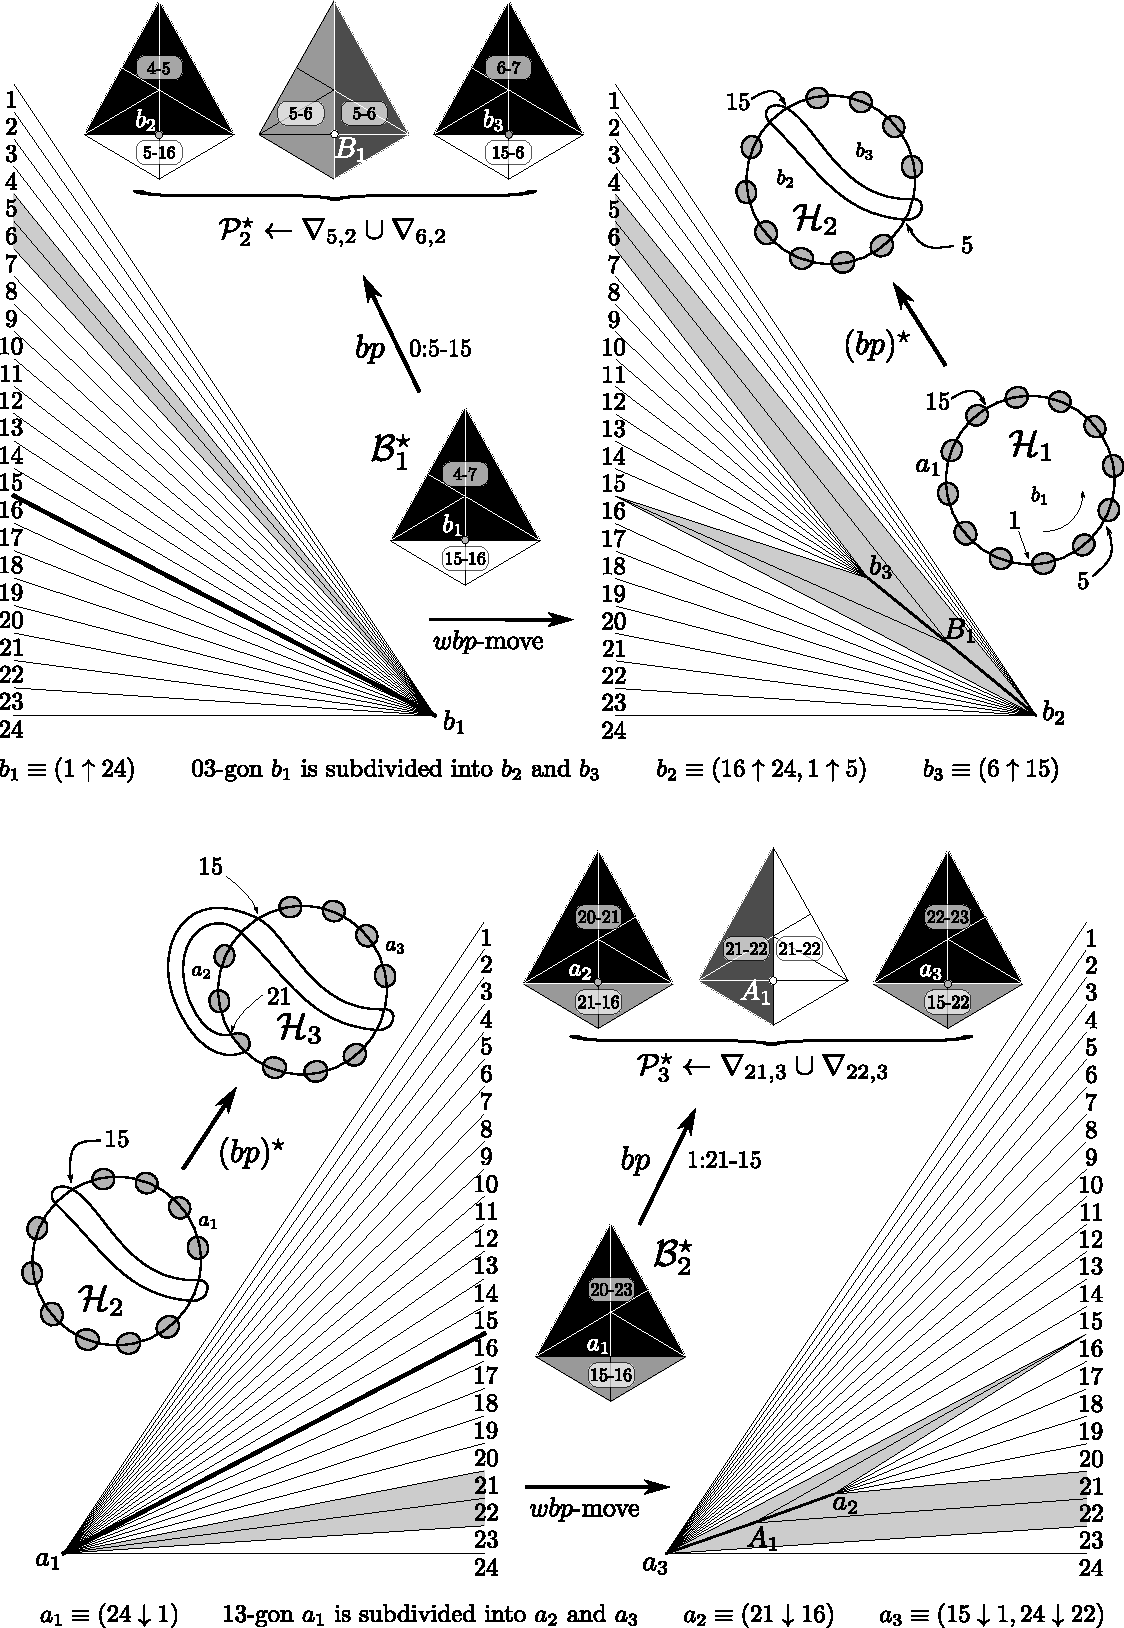
\includegraphics[width=15cm]{A.figs/bpandwinglist123.pdf} \\
\caption{\sf 
$\mathcal{H}^\star_{2} \leftarrow \mathcal{H}^\star_1 
\cup (\mathcal{P}_{2}^\star \backslash \mathcal{B}_1^\star)$. 
Pillow $\mathcal{P}_{2}^\star \leftarrow 
\nabla_{5,12}\cup \nabla_{6,12}$
($r^{24}_5$-example).}
\label{fig:winglist01}
\end{center}
\end{figure}
%-----------------------------------

%-----------------------------------
\begin{figure}
\begin{center}
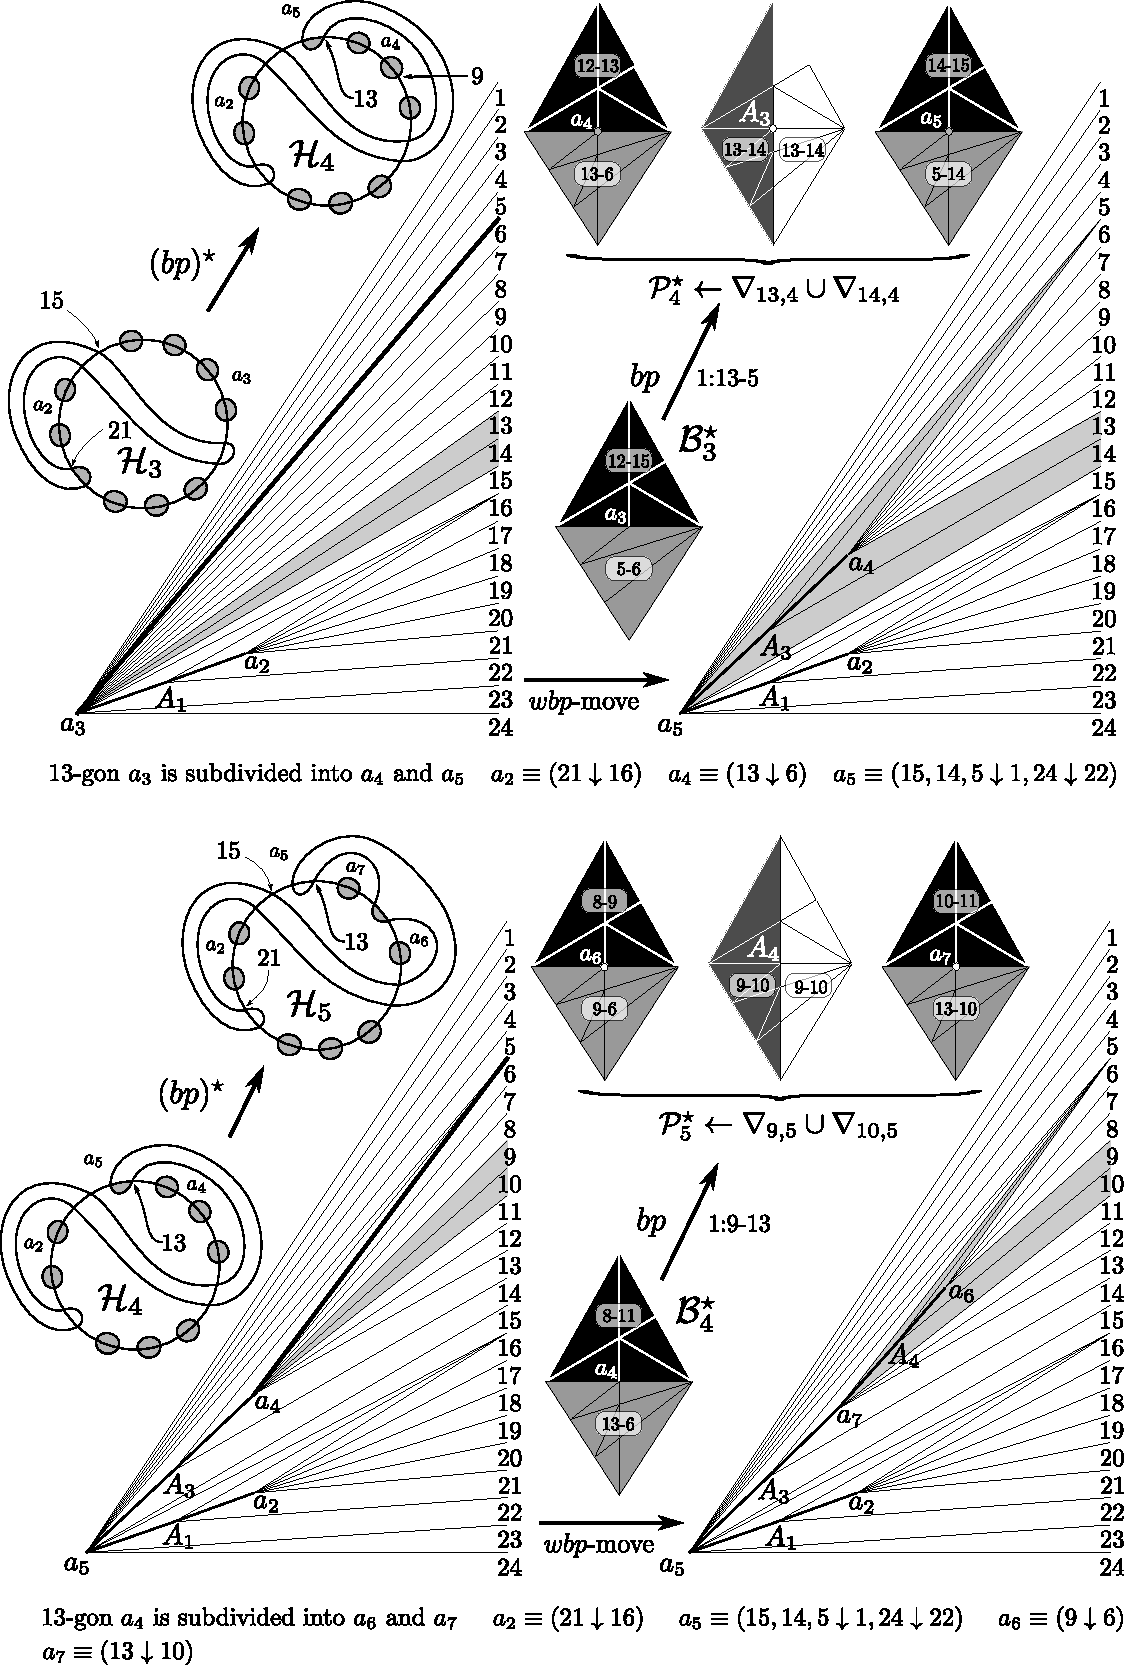
\includegraphics[width=15cm]{A.figs/bpandwinglist345.pdf} \\
\caption{\sf 
$\mathcal{H}^\star_{3} \leftarrow \mathcal{H}^\star_2 
\cup (\mathcal{P}_{3}^\star \backslash \mathcal{B}_2^\star)$. 
Pillow $\mathcal{P}_{3}^\star \leftarrow 
\nabla_{21,12}\cup \nabla_{22,12}$
($r^{24}_5$-example).}
\label{fig:winglist02}
\end{center}
\end{figure}
%-----------------------------------

%-----------------------------------
\begin{figure}
\begin{center}
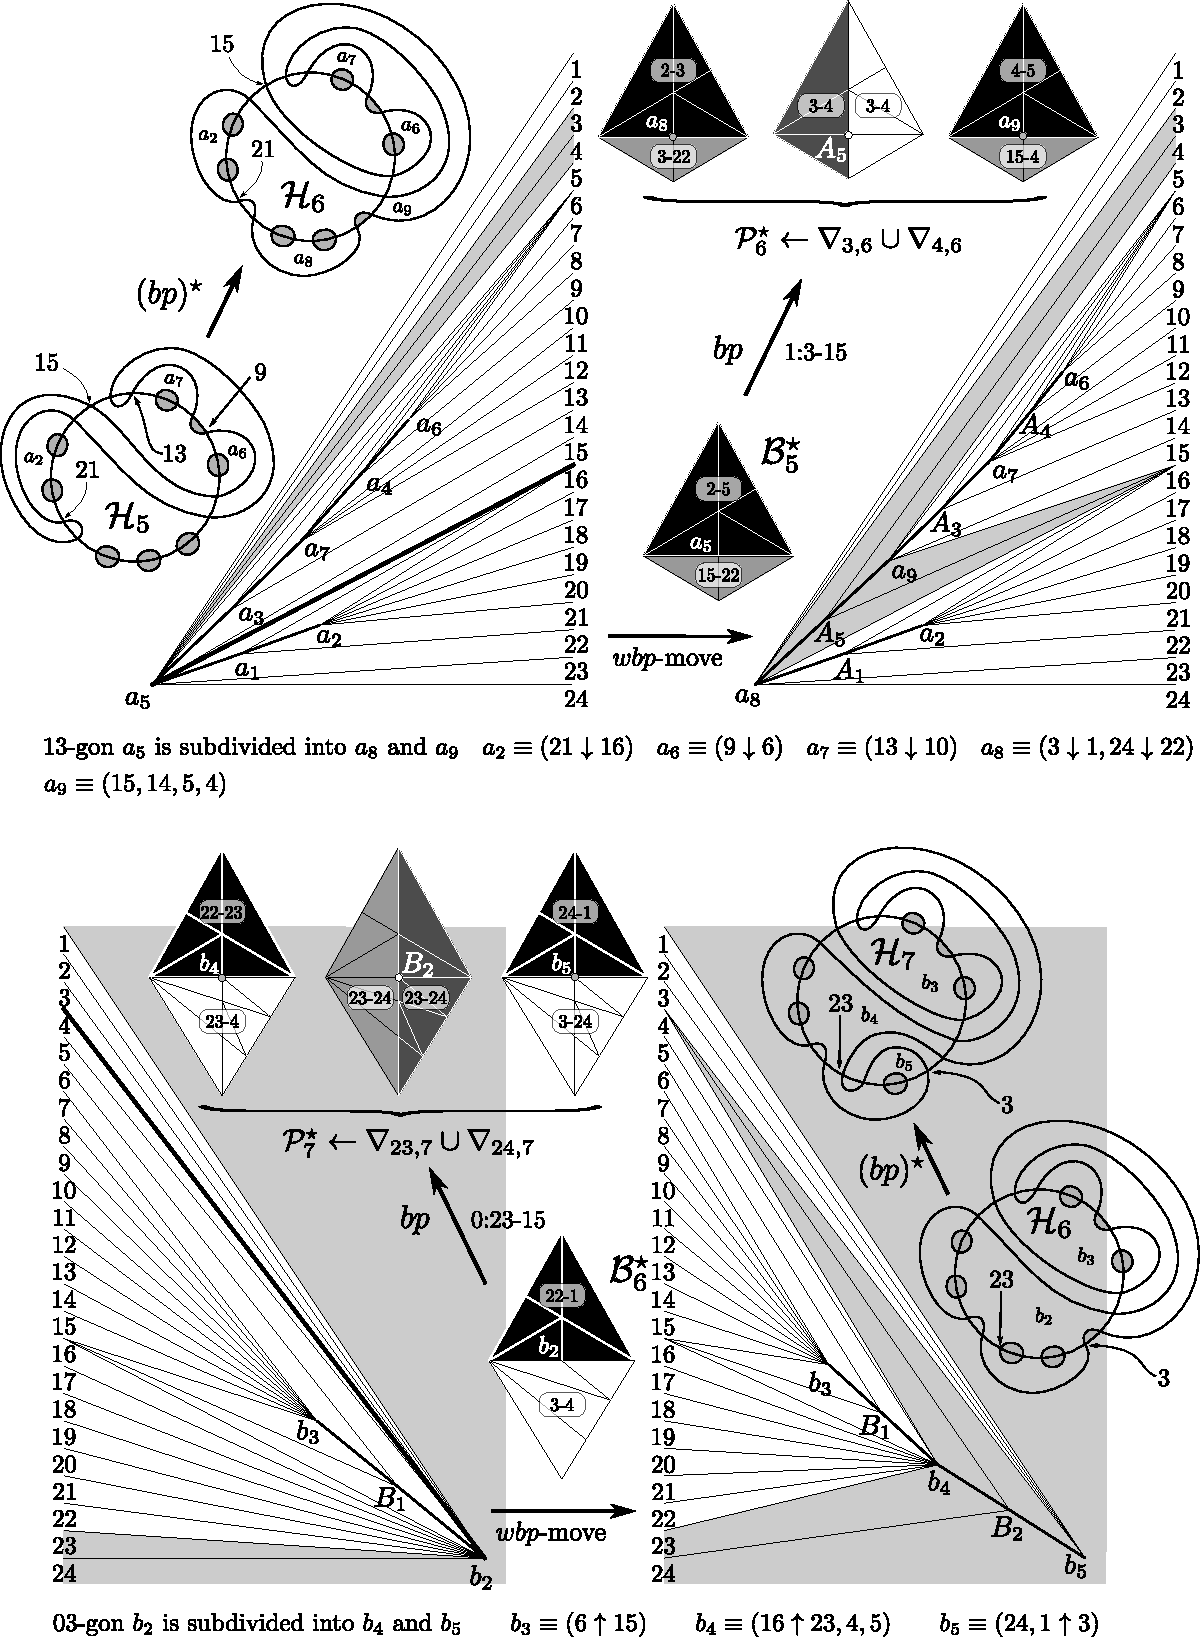
\includegraphics[width=15cm]{A.figs/bpandwinglist567.pdf} \\
\caption{\sf 
$\mathcal{H}^\star_{4} \leftarrow \mathcal{H}^\star_3 
\cup (\mathcal{P}_{4}^\star \backslash \mathcal{B}_3^\star)$. 
Pillow $\mathcal{P}_{4}^\star \leftarrow 
\nabla_{13,12}\cup \nabla_{14,12}$
($r^{24}_5$-example).}
\label{fig:winglist03}
\end{center}
\end{figure}
%-----------------------------------

%-----------------------------------
\begin{figure}
\begin{center}
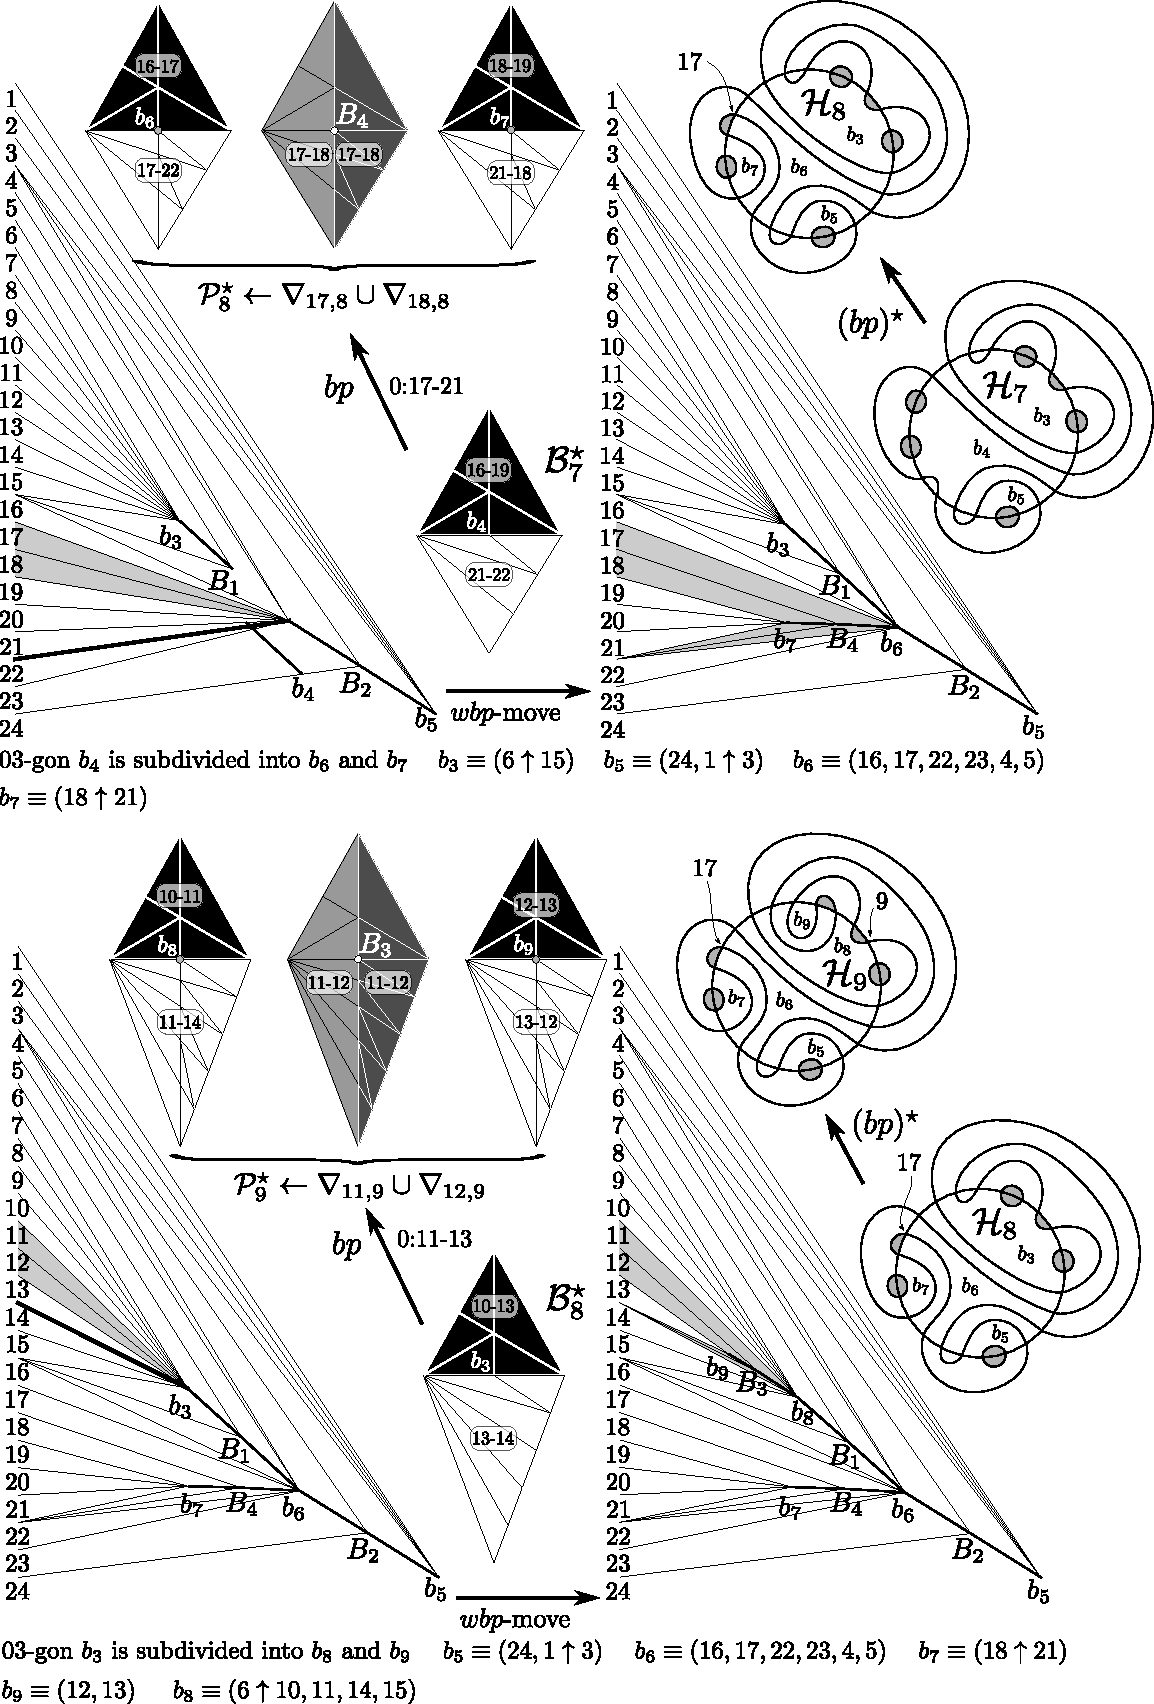
\includegraphics[width=15cm]{A.figs/bpandwinglist789.pdf} \\
\caption{\sf 
$\mathcal{H}^\star_{5} \leftarrow \mathcal{H}^\star_4 
\cup (\mathcal{P}_{5}^\star \backslash \mathcal{B}_4^\star)$. 
Pillow $\mathcal{P}_{5}^\star \leftarrow 
\nabla_{9,12}\cup \nabla_{10,12}$
($r^{24}_5$-example).}
\label{fig:winglist04}
\end{center}
\end{figure}
%-----------------------------------

%-----------------------------------
\begin{figure}
\begin{center}
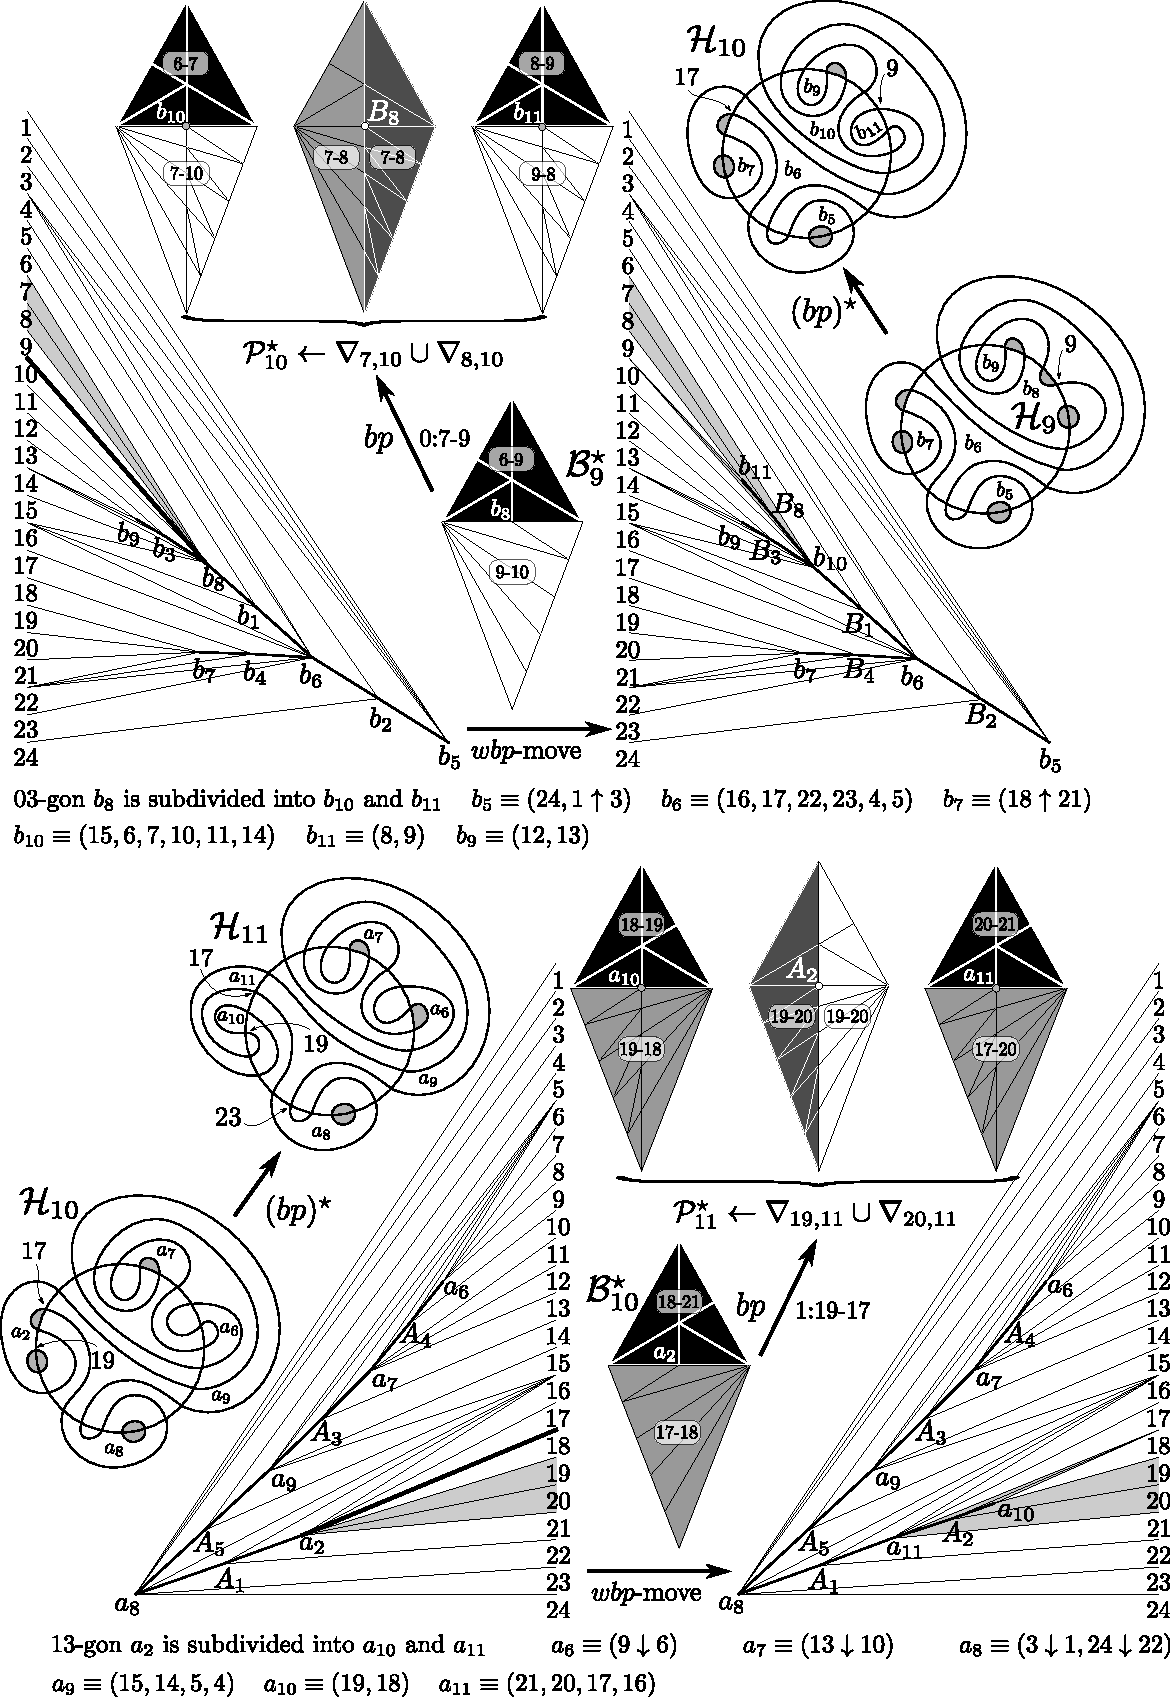
\includegraphics[width=15cm]{A.figs/bpandwinglist91011.pdf} \\
\caption{\sf 
$\mathcal{H}^\star_{6} \leftarrow \mathcal{H}^\star_5 
\cup (\mathcal{P}_{6}^\star \backslash \mathcal{B}_5^\star)$. 
Pillow $\mathcal{P}_{6}^\star \leftarrow 
\nabla_{3,12}\cup \nabla_{4,12}$
($r^{24}_5$-example).}
\label{fig:winglist05}
\end{center}
\end{figure}
%-----------------------------------

%-----------------------------------
\begin{figure}
\begin{center}
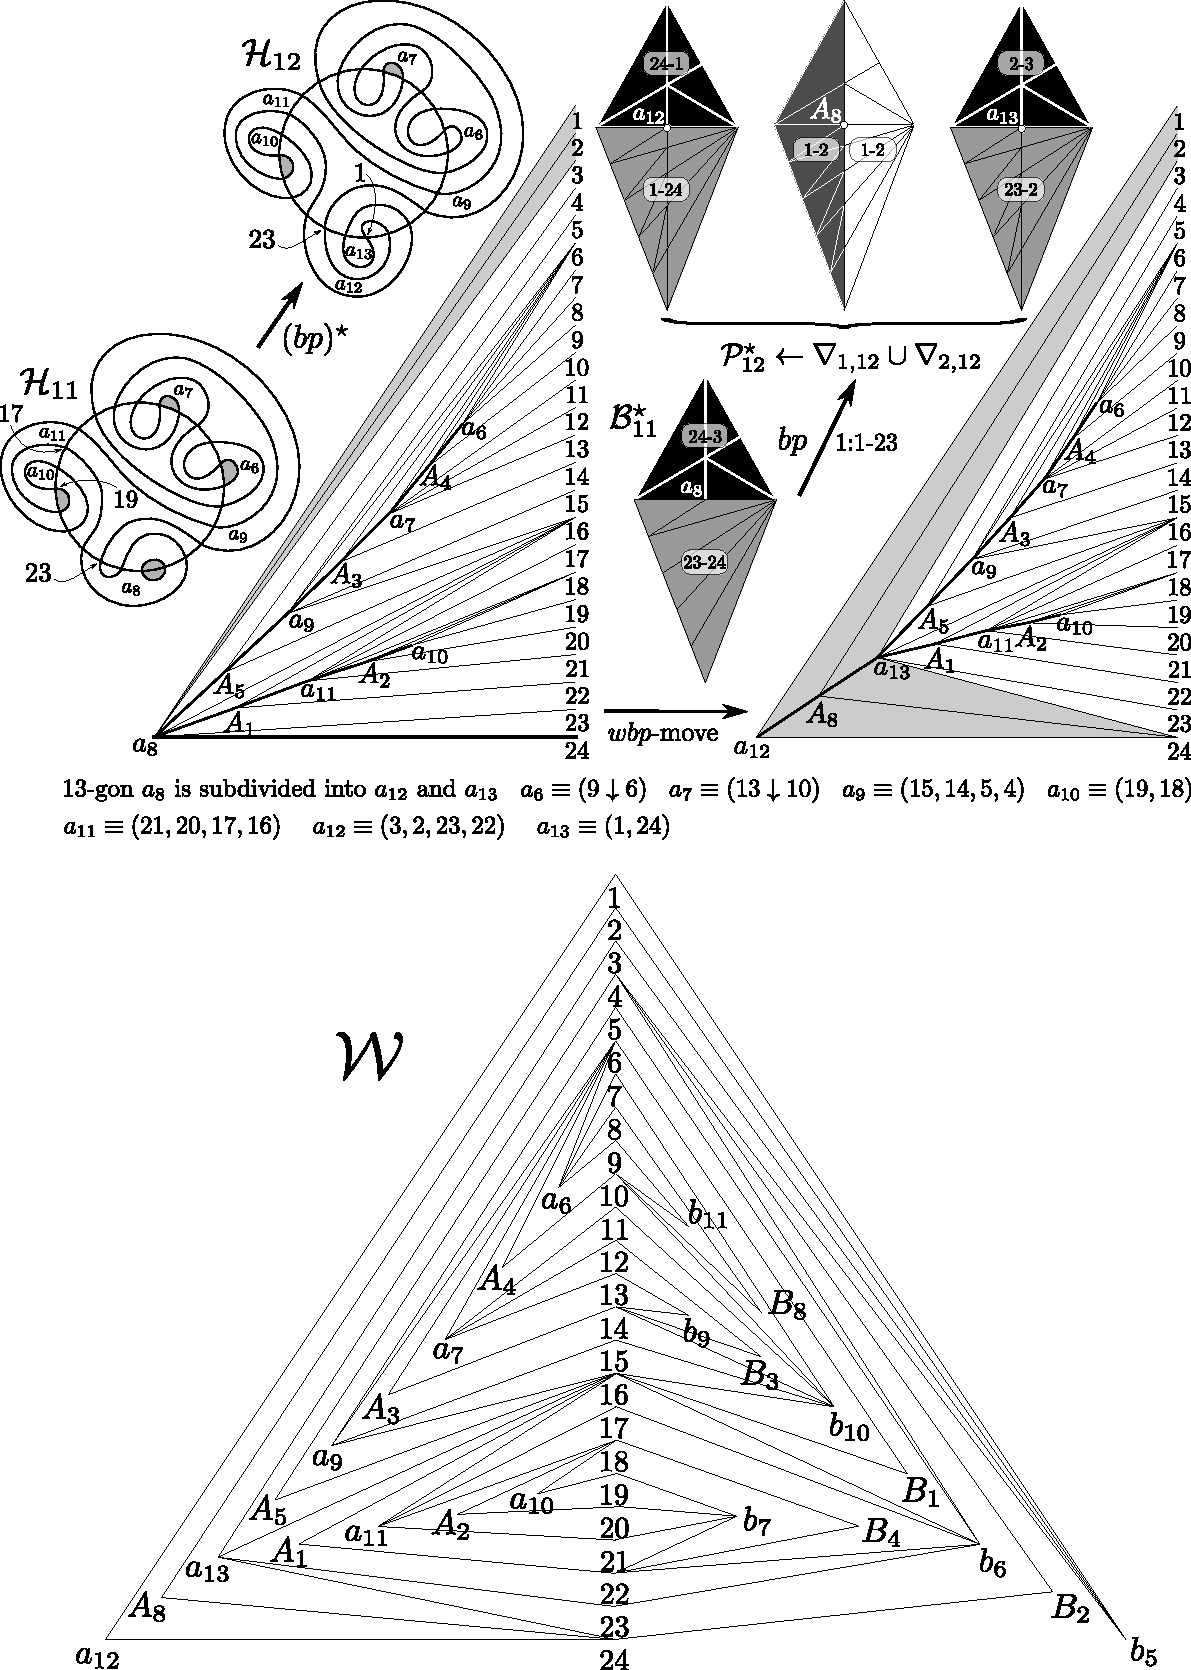
\includegraphics[width=15cm]{A.figs/bpandwinglist1112LW.pdf} \\
\caption{\sf 
$\mathcal{H}^\star_{7} \leftarrow \mathcal{H}^\star_6 
\cup (\mathcal{P}_{7}^\star \backslash \mathcal{B}_6^\star)$. 
Pillow $\mathcal{P}_{7}^\star \leftarrow 
\nabla_{23,12}\cup \nabla_{24,12}$
($r^{24}_5$-example).}
\label{fig:winglist06}
\end{center}
\end{figure}
%-----------------------------------


%-----------------------------------
\begin{figure}[H]
\begin{center}
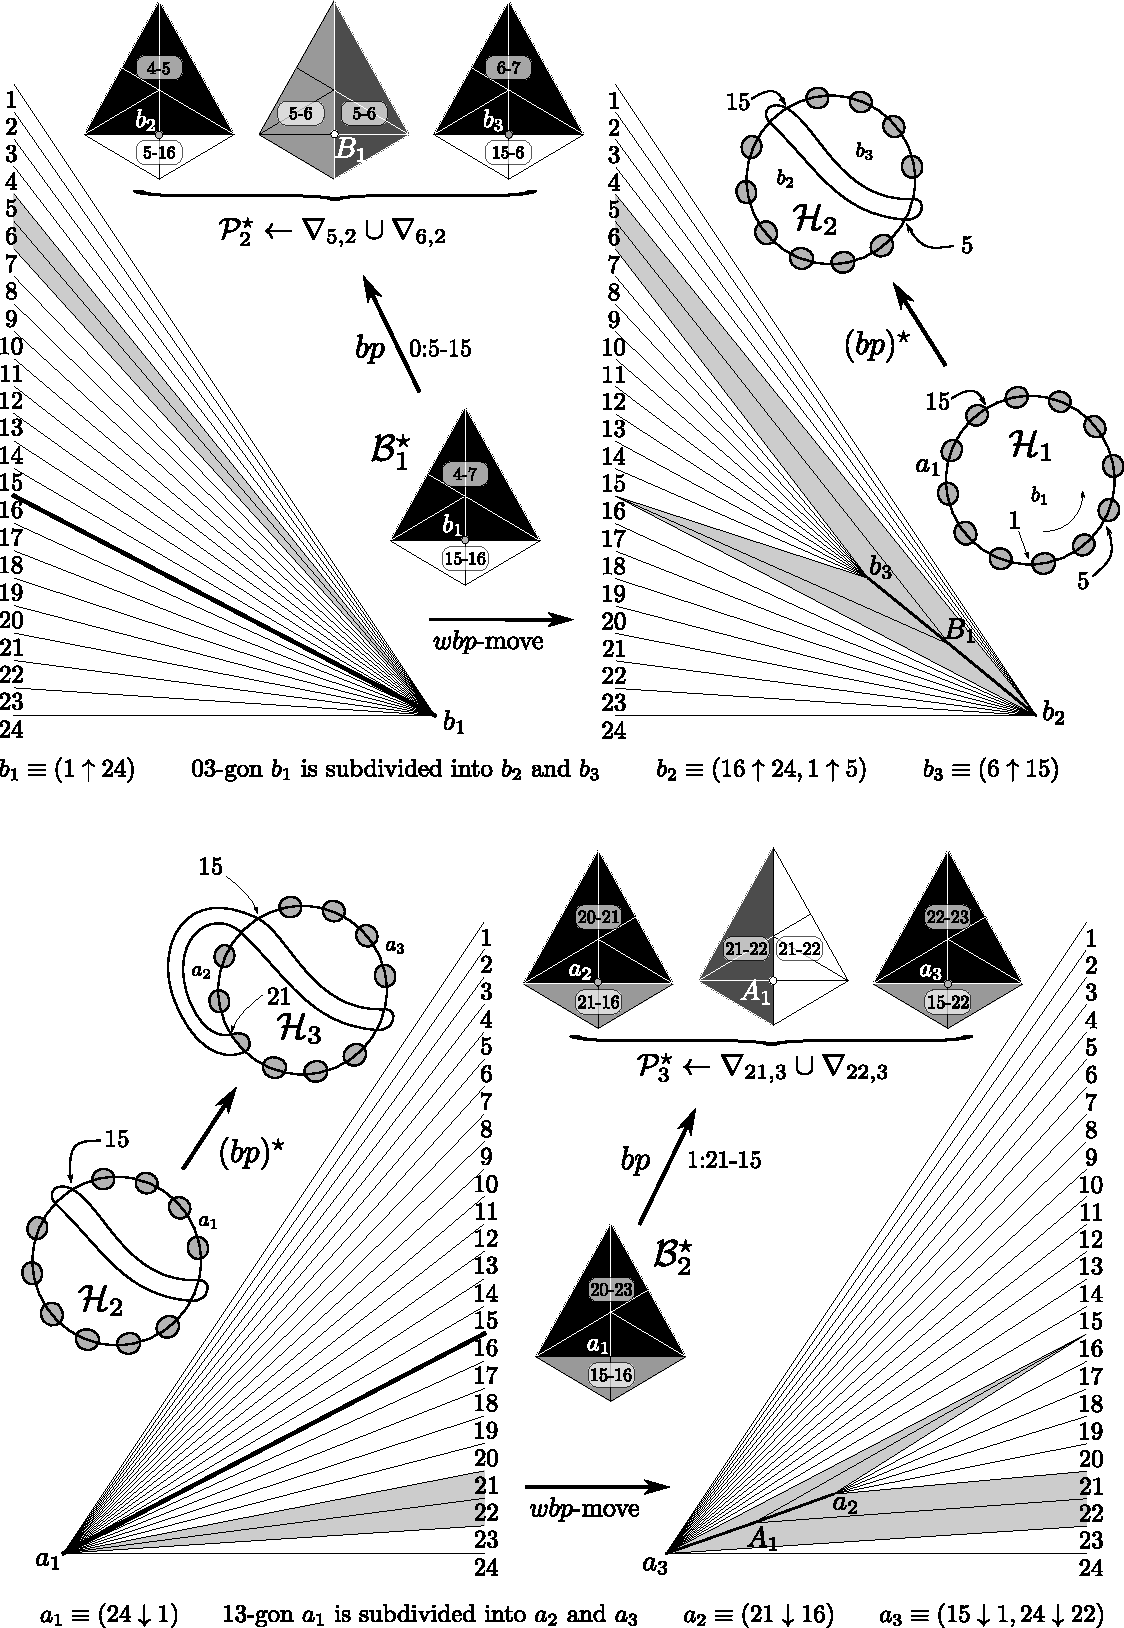
\includegraphics[width=15cm]{A.figs/bpandwinglist123.pdf} \\
\caption{\sf The initial right wing $\mathcal{W}''_1$
is a pincel of lines emanating from $b_1$.
The initial right nervure $\mathcal{N}''_1$ is empty. 
The initial left wing $\mathcal{W}'_1$
is a pincel of lines emanating from $a_1$.
The initial left nervure $\mathcal{N}'_1$ is empty.
At the end of each $wpb$-move a pair of edges is added to the nervure.
Lower case symbols $a_j, b_k$ refer to 13-gons and 03-gons. Upper case symbols
$A_j, B_k$ are auxiliary 0-simplexes.
}
\label{fig:winglist01}
\end{center}
\end{figure}
%-----------------------------------

%-----------------------------------
\begin{figure}[H]
\begin{center}
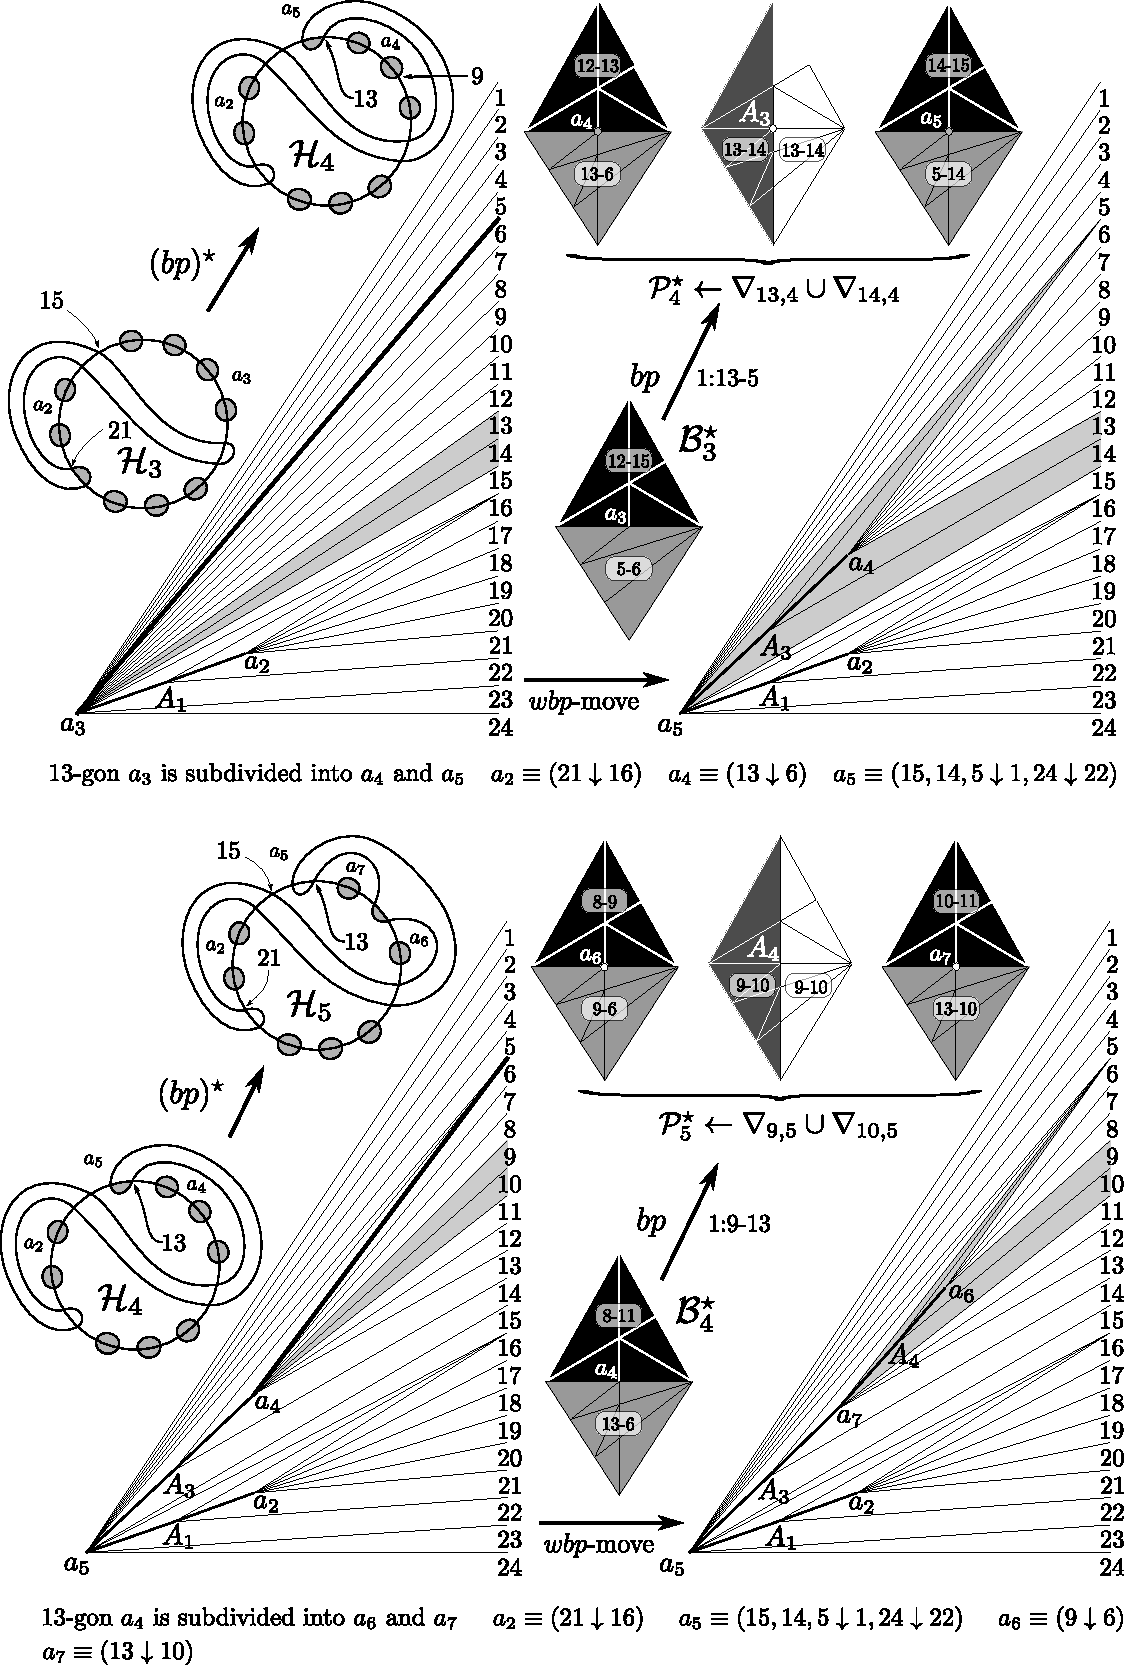
\includegraphics[width=14.1cm]{A.figs/bpandwinglist345.pdf} \\
\caption{\sf A left strut is modified by a $wbp$-move. What is needed as input 
is a pair of adjacent 
shaded triangles and a thick edge. In the lower the left strut is further 
modified by another $wbp$-move. The modification of balloons into pillows define the new
colored abstract combinatorial complexes. The nervures $\mathcal{N}_m$ are auxiliar devices
that will be disposed after we find the rectilinear embedded
$\mathcal{W}$ by a deterministic linear algorithm,
See Fig. \ref{fig:winglist06}.}
\label{fig:winglist02}
\end{center}
\end{figure}
%-----------------------------------

%-----------------------------------
\begin{figure}[H]
\begin{center}
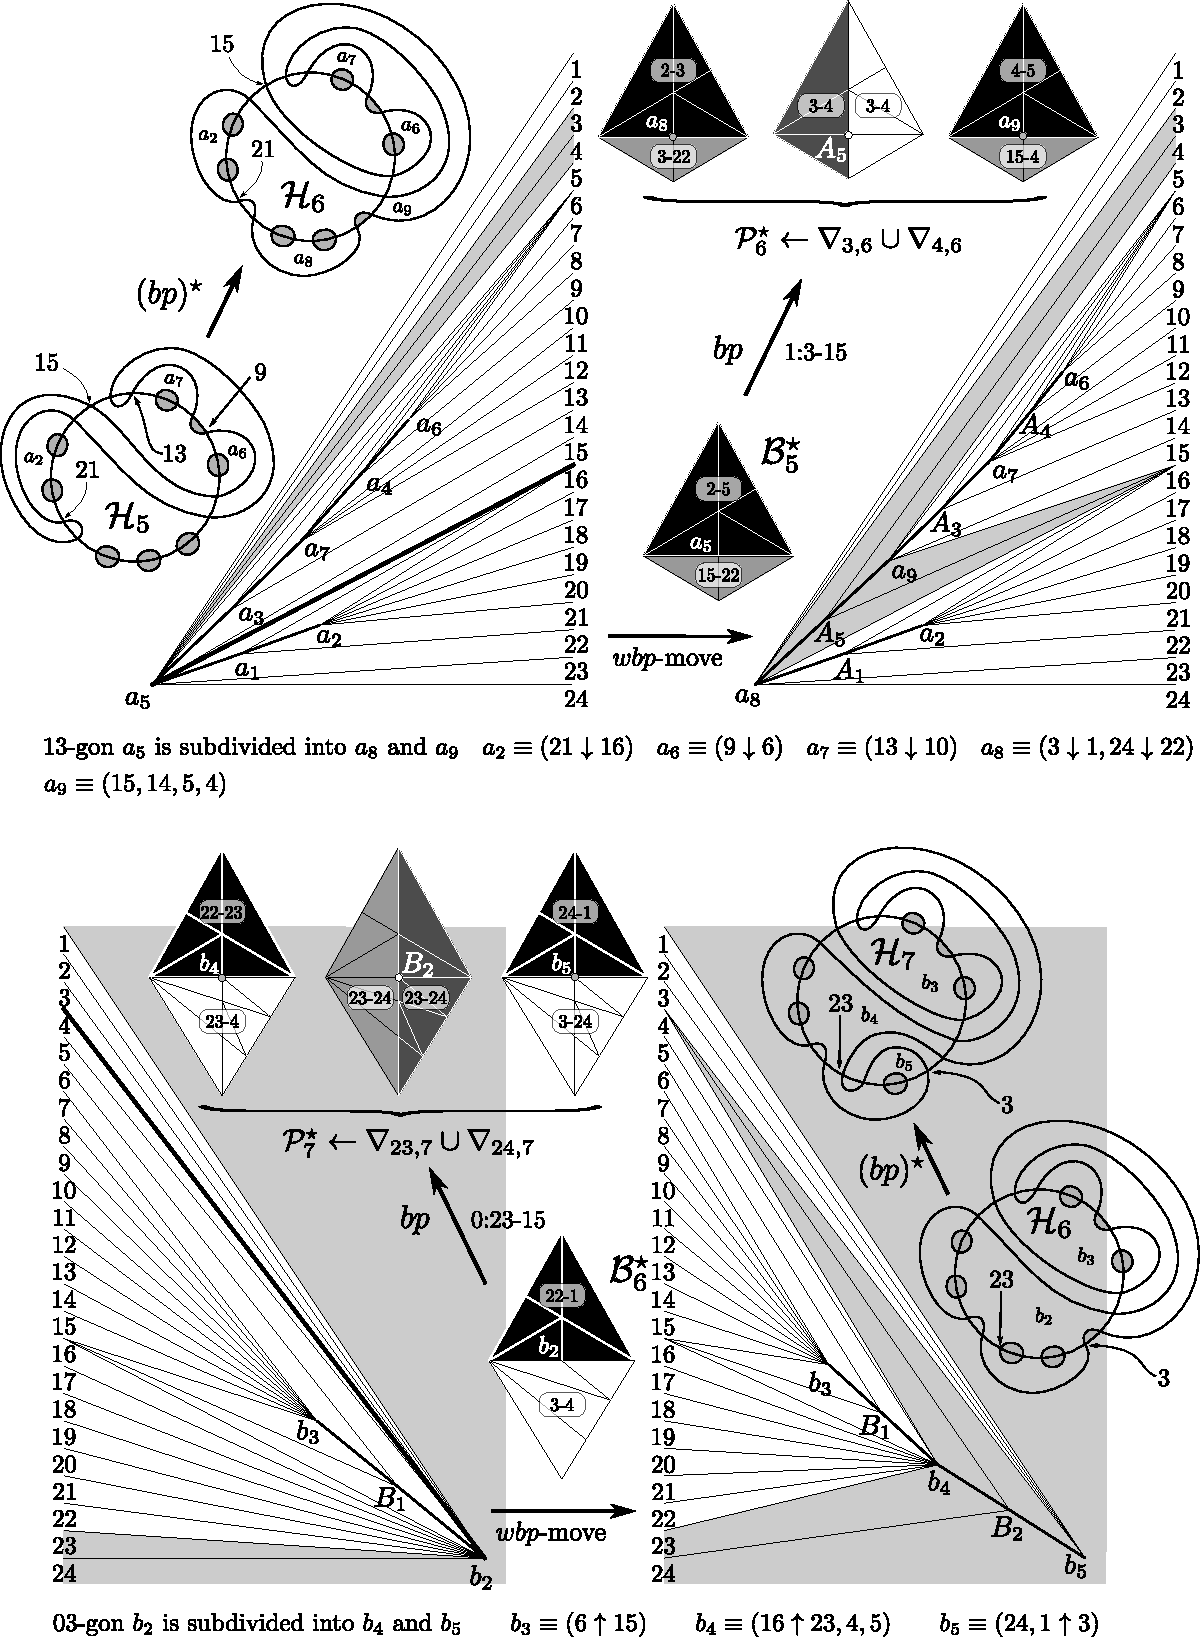
\includegraphics[width=15cm]{A.figs/bpandwinglist567.pdf}
\caption{\sf
In the first $wbp$-move a left strut is {\em extended based on $a_5$}. 
In all the figures of this $r^{24}_5$-example (except for the $\mathcal{W}$ at the last one) 
we have used Tutte's barycentric
method \cite{tutte1963dg,colin2003tutte} to obtain the embedded final struts. 
However, except for $\mathcal{W}$, only the combinatorics of the embeddings (the rotations)
are needed to encode the struts in an implementation of the algorithm.
In the second $wbp$-move one of the two shaded triangles
is in the outside. Depite this special case, the rotation manifestation of the 
move behaves as usual.
}
\label{fig:winglist03}
\end{center}
\end{figure}
%-----------------------------------

%-----------------------------------
\begin{figure}[H]
\begin{center}
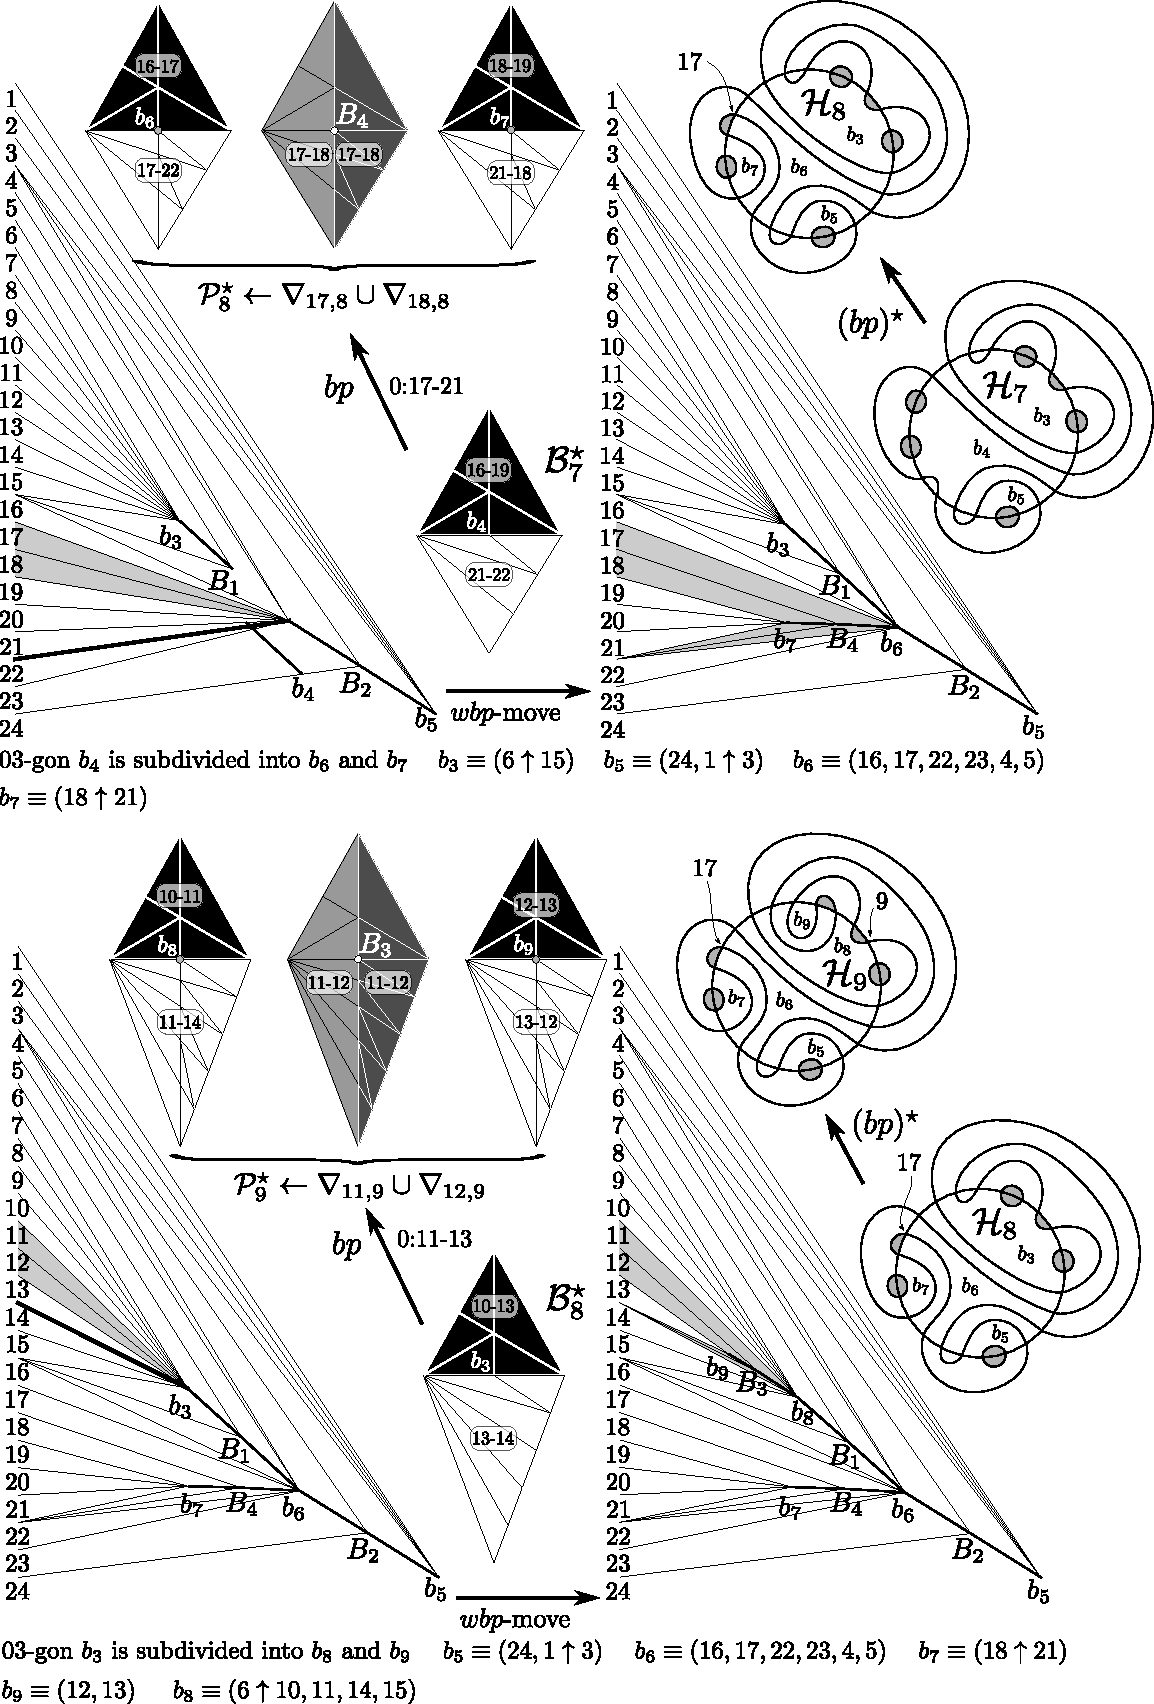
\includegraphics[width=14.7cm]{A.figs/bpandwinglist789.pdf} \\
\caption{\sf The first $wbp$-move induces a bifurcation on the nervure of a
right wing based on $b_4$. 
The second $wbp$-move produces an extension based on $b_3$ 
of the nervure of the final right
wing of the first $wbp$-move.
}
\label{fig:winglist04}
\end{center}
\end{figure}
%-----------------------------------

%-----------------------------------
\begin{figure}[H]
\begin{center}
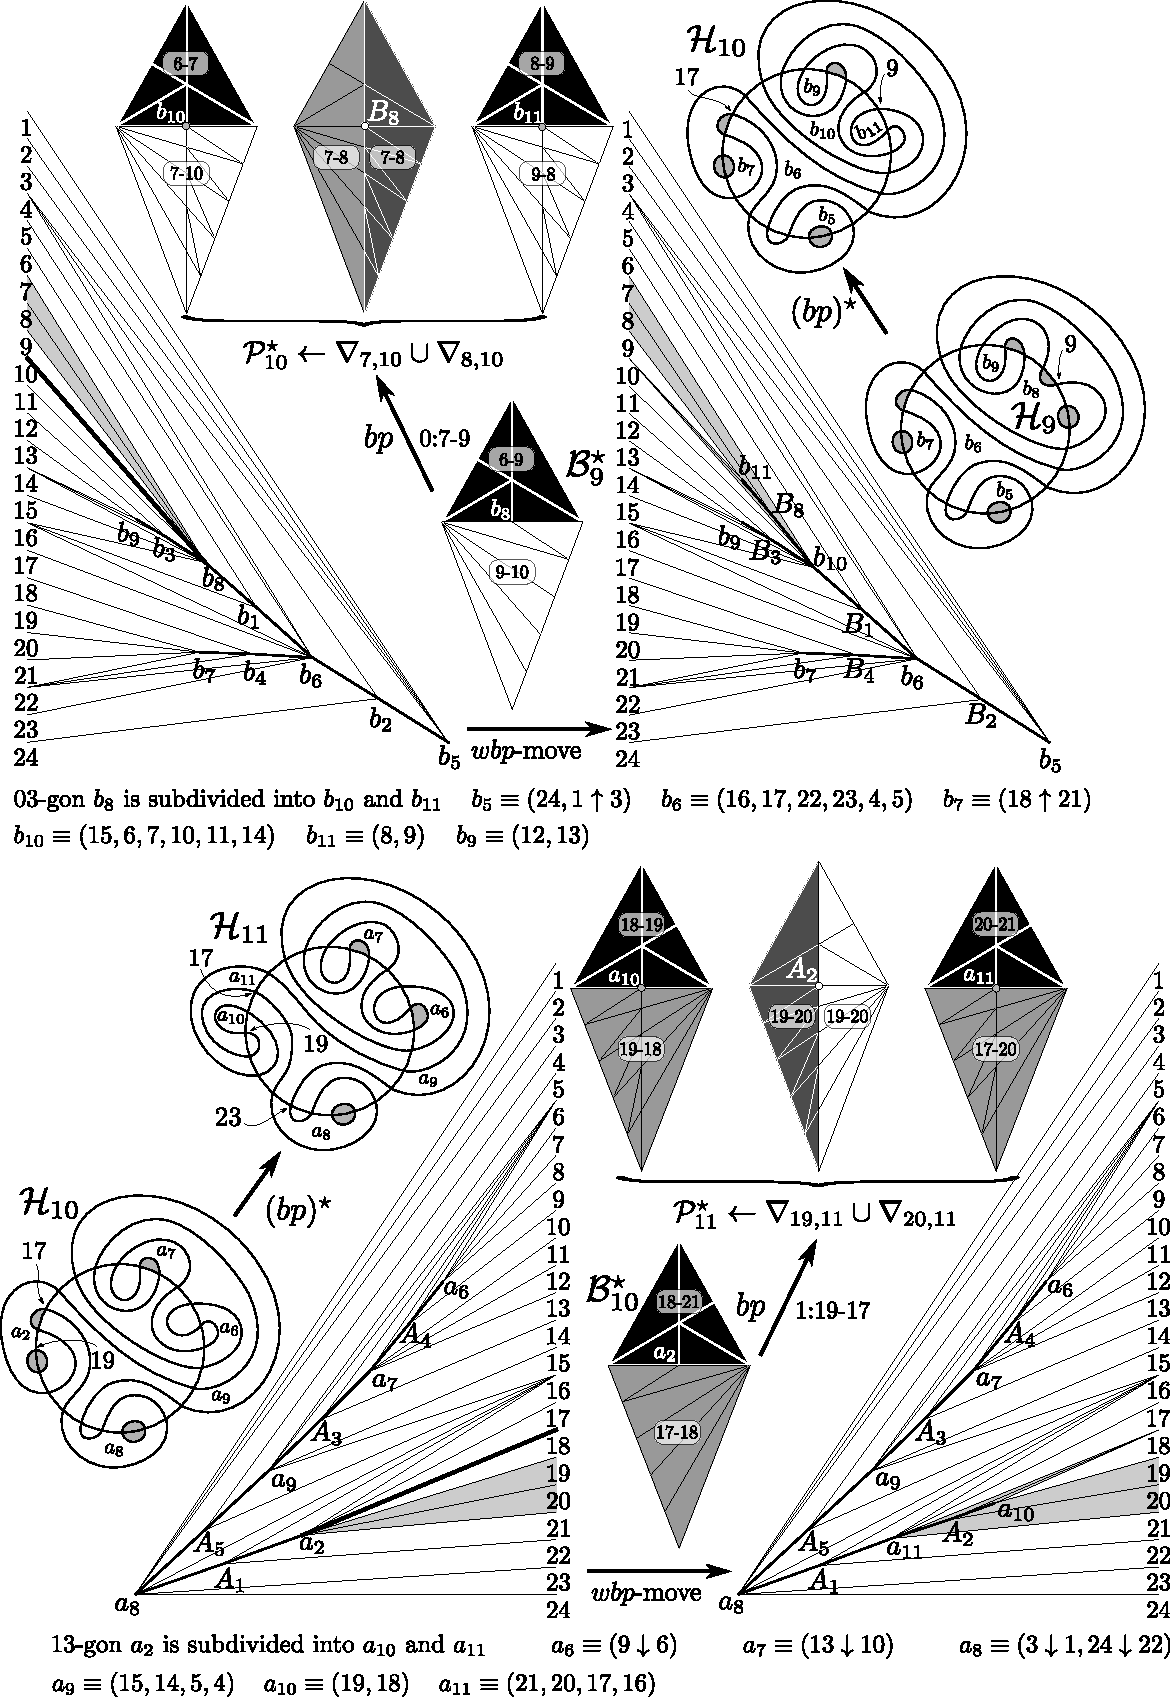
\includegraphics[width=15cm]{A.figs/bpandwinglist91011.pdf} \\
\caption{\sf The first $wbp$-move induces another bifurcation on the nervure of a
right wing based in $b_8$. The second $wbp$-move 
produces an extension of the nervure of a left
wing based on $a_2$.}
\label{fig:winglist05}
\end{center}
\end{figure}
%-----------------------------------

%-----------------------------------
\begin{figure}[H]
\begin{center}
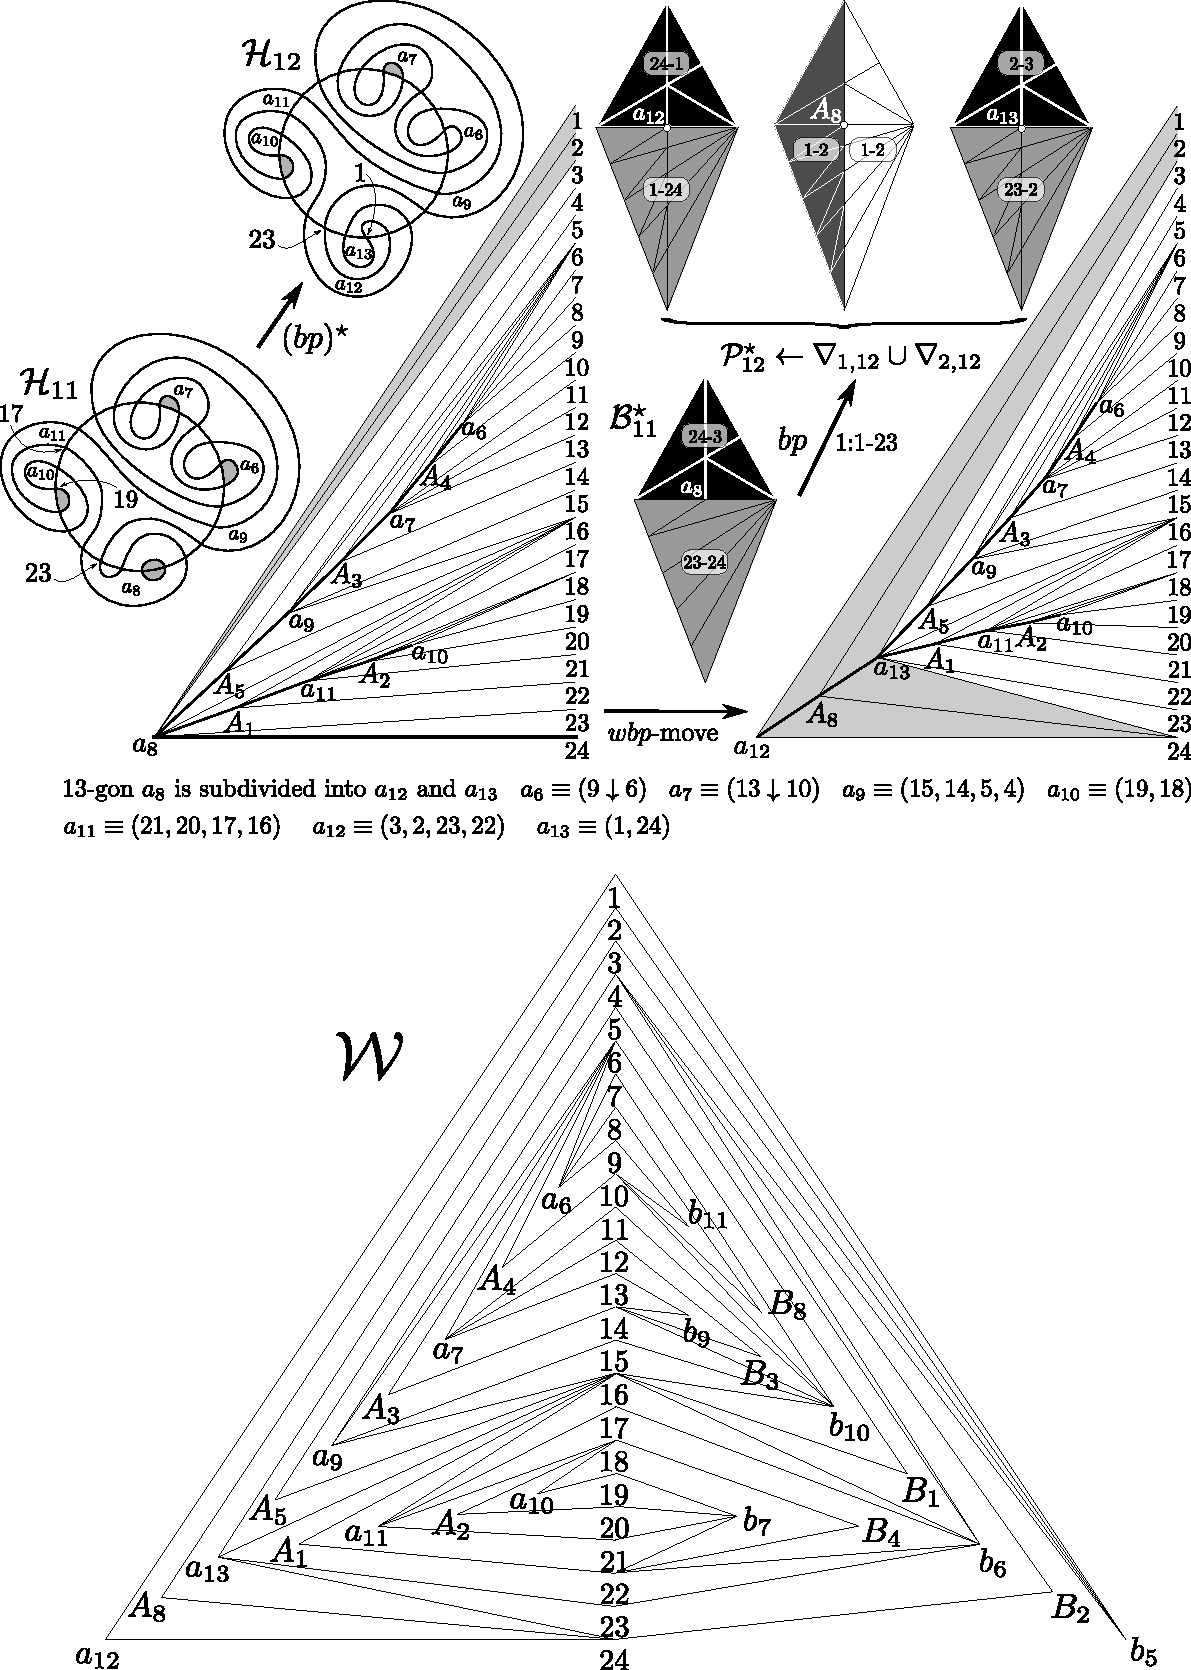
\includegraphics[width=14.5cm]{A.figs/bpandwinglist1112LW.pdf} \\
\caption{\sf The globally last $wbp$-move is the extension based at $a_8$ 
(correponding to a 13-gon which breaks into two $a_{12}$ and $a_{13}$). The bottom part of
the figure despict the final pair of wings $\mathcal{W}$. For this object we have
a rectilinear embedding based on the deterministic 
linear algorithm which we explain in Section{??}.
Obtaining this embedding by a linear deterministic 
algorithmic is central for our purposes. The passage 
$\mathcal{W} \rightarrow \mathcal{H}_1^\diamond$ is straighforward by a cone algorithm.
}
\label{fig:winglist06}
\end{center}
\end{figure}
%-----------------------------------

%-----------------------------------
\begin{figure}[H]
\begin{center}
\includegraphics[width=14.5cm]{A.figs/Wdiamond1.pdf} \\
\caption{\sf To get $\mathcal{W}^\diamond_1=\mathcal{W}^{\diamond'}_1 
\cup \mathcal{W}^{\diamond''}_1$ from $\mathcal{W}$ remove
all but two straight line segments emanating from  $z_3^k$, one in each side.
The two segments that survive are the ones finishing at the smallest index upper case $A_p$
and the smallest indexed upper case $B_q$.
Let $\{x\} \cup Y \subseteq \mathbb{R}^N$, for $1\le N \in \mathbb{N}$. 
The \index{cone} {\em cone} \cite{rourke1982introduction} 
with vertex $x$ and base $Y$, denoted $x \ast Y \subseteq \mathbb{R}^N$,
is the union of $Y$ with all line 
segments which link $x$ to $y \in Y$.
The passage 
$\mathcal{W}_1^ \diamond \rightarrow \mathcal{H}_1^\diamond$ is 
straighforward by a cone algorithm:
for each $e'\in \mathcal{W}_1^{\diamond'}$ add the two 2-simplices $z_0\ast e'$ and $z_2\ast e'$
to $\mathcal{H}^\diamond_1$;
for each $e''\in \mathcal{W}_1^{\diamond''}$ add the two 2-simplices $z_1\ast e''$ and $z_2\ast e''$
to $\mathcal{H}^\diamond_1.$ 
To complete $\mathcal{H}^\diamond_1$ add the 2-simplices $\{z_3^jz_1z_0 ~|~ j=1, \ldots, 2n \}.$
}
\label{fig:Wdiamond1}
\end{center}
\end{figure}
%-----------------------------------


\subsection{Acknowledgements}
We thank the anonimous referees, which made us think and provide an $O(n)$-solution
for finding the wing sequence, instead of an $O(n^3)$-solution based on a bare Tutte's
barycetric methods.

\section{Details of the whole construction}
\subsection{First phase: from a $J^2$-gem $\mathcal{H}$ to a bloboid $\mathcal{B}$}

A $k$-dipole $\{u,v\}$ involves color $i$ if it 
if there is an edge of color $i$ linking $u$ to $v$.

Let $H$ be the $J^2$-gem formed by the two Jordan curves $X$ and $Y$.
A {\em $(X,Y)$-duet} in $H$ is a pair of crossings which are consecutive in $X$ and in $Y$.
A {\em $(X,Y)$-trio} in $H$ is, likewise, a triple of crossings that 
are consecutive in $X$ and in $Y$.

\begin{lemma}
\label{lem:trio}
Let $H$ be a $J^2$-gem with $2n\geq4$ vertices. Then $H$ has a $(X,Y)$-trio. 
\end{lemma}
\begin{proof}
By the Jordan theorem $H$ has a $(X,Y)$-duet $D$. If $n=2$ then $H$ has clearly a 
$(X,Y)$-trio establishing the basis of the induction.
Suppose $H$ has $2n\geq 4$ vertices. It has a $(X,Y)$-duet $D$.
If $D$ extends to a trio, then we are done.
Otherwise slightly deform $Y$ to miss $D$. The resulting
$J^2$-gem $H'$ has $2n-2$ crossings and by induction hypothesis $H'$ has a $(X,Y)$-trio $T$,
which is present in $H$, establishing the Lemma.
\end{proof}

\begin{proposition}
\label{prop:startingwith}
Starting with a $J^2$-gem $\mathcal{H}$ with $2n$ vertices we can arrive to an
$n$-bloboid $\mathcal{B}$ by means of $n-1$ operations which 
thickens a 2-dipole involving color 2 into a 3-dipole, where the new edge is of color 0 or color 1,
producing a sequence of $J^2B$-gems each inducing $\mathbb{S}^3$,
$$(\mathcal{H}=\mathcal{H}_{n},\mathcal{H}_{n-1},\ldots, 
\mathcal{H}_{2},\mathcal{H}_{1}=\mathcal{B}).$$

\end{proposition}
\label{prop:backsequence}
\begin{proof}
The proof is by backward induction. 
For $\ell=n$ we have $\mathcal{H}_{n}=\mathcal{H}$ and
so it is a $J^2B$-gem, establishing the basis of the induction. Assume that
$\mathcal{H}_\ell$ is a $J^2B$-gem.
For $\ell>1$, let $\mathcal{H}'_\ell$ denote  $\mathcal{H}_\ell$ after cancelling the blobs.
By Lemma \ref{lem:trio} $\mathcal{H}_\ell'$ has a $(X,Y)$-trio $(x,y,z)$. Thus $y$
is incident to two 2-dipoles. One of these dipoles, call it $D$,
involves color 2, the other involves color 3.
Take the one involving color 2, name it $D$. Put back the blobs over the edges of color 3.
So, $D$ is present in $\mathcal{H}_\ell$. The colors involved in 
$D$ are $0$ and $2$ or $1$ and $2$. In the first case we use color 1 to thicken $D$ and
in the second we use color $0$ for the same purpose.
This defines the $J^2B$-gem $\mathcal{H}_{\ell-1}$, which
establishes the inductive step. In face of Proposition \ref{prop:j2shere} and from
the fact that thickening dipoles on gems produce gems inducing the same manifold, 
every member of the sequence induces $\mathbb{S}^3$.
\end{proof}

% The above proof is illustrated in Fig. \ref{fig:j2gemrSEQ}. Note that the thickenings are of two
% types: either of type $0$ where the edges $e$ and $f$ are $0$-edges in the interior of the $23$-gon, or else
% of type $1$ if they  are $1$-edges in its exterior. The above sequence is by no means unique because
% various 2-dipole choices present themselves along the way. We fix one and such a sequence and 
% used it as the basis for
% establishing bounds on the size of the colored complexes, 
% dual of the $J^2$-gem. This is done in the companion
% paper \cite{linsmachadoB2012}.

\subsection{Second phase: colored abstract complexes, their wings, nervures}
The second phase starts with an easy task, namely to define the dual of the bloboid,
named $\mathcal{H}_1^{\star}$. We get this first term in an embedded form. 
The others $\mathcal{H}_2^{\star}$, \ldots, $\mathcal{H}_n^{\star}$,
are, at this stage, obtained by slight modifications of the antecessor, but only in 
an abstract compinatorial way. In doing so we get the minimum 
level of refinement in the PL2-faces required, so that latter, the levels are sufficient
for a geometric PL-embedding in $\mathbb{R}^ 3$ which we seek.


\subsubsection{Primal and dual correspondence between the gem and the colored complex}
There is a simple topological interpretation between primal and dual complexes, given in 
\cite{lins1995gca} pages 38, 39. Let us take a look 
at this interpretation in our context. This will help 
 to understand the $PL$-embedding $\mathcal{H}_m^\star$.
In what follows the $k$ in PL$k$-face means the dimension $k\in\{0, 1, 2,3\}$ of the PL-face.

\begin{itemize}
 \item [i.] 
a vertex $v$ in $G$ $\rightleftharpoons$ a 
solid PL-tetrahedron or PL3-face,
denoted by $\nabla_v$ in the dual of the gem whose
PL0-faces are labelled $z_0$, $z_1$, $z_2$ e $z_3^v$; 
in this work, it is enough to work with the 
boundary of a PL3-face; this is topologically a sphere
$\mathbb{S}^2$ with four PL2-faces one of each color; the 3-simplices forming
a PL3-face need not be explicitly specified;
 \item [ii.] an $i$ colored edge $e_i$ in $G$ $\rightleftharpoons$ a set 
of $i$-colored 2-simplices defining 
a PL2$_i$-face in the dual of the gem;
 \item [iii.] a bigon $B_{ij}$ using the colors $i, j$ in 
$G$ $\rightleftharpoons$ a set of  1-simplices $b_{ij}$
 in $\mathcal{H}_n^\star$ defining a 
PL1$_{ij}$-face;
 \item [iv.] an $\overline{i}$-residue $V_i$ in $G$ 
$\rightleftharpoons$ a 0-simplex in $\mathcal{H}_n^\star$ defining a PL0$_i$-face.
\end{itemize}

\subsubsection{Defining $\mathcal{H}_1^\star$ and the colored abstract PL-complexes: 
$\mathcal{H}_2^{\star}$, \ldots, $\mathcal{H}_n^{\star}$}

We define the combinatorial 2-dimensional PL complex $\mathcal{H}_1^{\star}$ as follows.
%Let $j \in \{1, \ldots, 2n\}$, define $v_0^j, v_1^j$ and $v_2^j$ as the vertices of $2n$ 
%equilateral triangles and subdivide as in 
 %defining $v_3^j, v_4^j$ and $v_5^j$. The scheme of colors
%depends of parity, if $j$ is odd, all the triangles are 3-colored, 
%otherwise triangles $v_0^jv_3^jv_1^j$ are 2-colored, defining the PL2$_2$-faces, 
%triangles $v_0^jv_4^jv_3^j$ and $v_2^jv_3^jv_4^j$ 
%are 1-colored, defining the 
%PL2$_1$-faces, and the triangles $v_1^jv_3^jv_5^j$ and $v_2^jv_5^jv_3^j$ are 0-colored, defining the PL2$_0$-faces.

%-----------------------------------
\begin{figure}[H]
\begin{center}
\includegraphics[scale=1]{A.figs/dualPL2.pdf}
\caption{\sf PL2-faces of $\mathcal{H}^\star_1$: the figure is an abreviation of a stack
of tetrahedra, where $k = 0,1,\ldots,n-1.$ The 0-simplices 
$z_3^j$ are defined as $z_3^j=(0,0,2n-j)$, $1\le j \le 2n$. For even $j=2k$,
there are five simplices incident to $z_3^j$: two 0-colored, two 1-colored and 1 2-colored.
For odd $j=2k+1$, the five 2-simplices incident to $z_3^j$ are all 3-colored.
The 0-simplices $z_0$, $z_1$ and $z_2$ are positioned in clockwise order 
as the vertices of an equilateral triangle 
of side 1 in the 
$xy$-plane so that $z_0z_1$ is parallel to the $x$-axis and the center of the triangle
coincides with the origin of an $\mathbb{R}^3$-cartesian system. 
The 0-simplex $a_1$ is $\frac{z_0+z_2}{2}$. The 0-simplex
$b_1$ is $\frac{z_2+z_1}{2}$. Note that, in general, the PL3-faces are given
by their boundary. We never use 3-simplices explicitly to triangulate the PL3-faces.
From our construction, however, it will be clear that this is possible to achieve
without spurious intersections among the 3-simplices.
}
\label{fig:dualPL2}
\end{center}
\end{figure}
%-----------------------------------

We detail the connection of the $J^2$-gem and its dual. In particular we 
use the unique 23-gons of it to provide labels $1,2,\ldots,2n$ in the cyclic 
order of the 23-gon. This labellings correpond to PL3-faces of the 
$\mathcal{H}_1^{\star}$ and will be maintained for the PL3-faces 
of the whole remaining sequence $\mathcal{H}_2^{\star}$, 
\ldots, $\mathcal{H}_n^{\star}$. This invariance is a dual 
manifestation of the fact that in
the thickening of dipoles the labels of the vertices preserved.
Suppose $u$ is an odd vertex of the $J^2$-gem, $u'=u-1$, $v=u+1$ and $v'= v+1$.
The dual of a $\overline{3}$-residue is $z_3^j$ where $j$ is even. 
When $j$ is odd, then $z_3^j$ is a $0$-simplex in the middle of a PL2$_3$-face,
incident to five 2-simplices of color 3.
The dual of the 03-gon is the PL1-face formed by the pair of 1-simplices $z_1b_1$ 
and $b_1z_2$. The dual of the 13-gon is the PL1-face formed by the pair of 
1-simplices $z_0a_1$ and $a_1z_2$. 
The dual of the 23-gon is the PL1-face formed by the 1-simplex $z_0z_1$.
The dual of the 01-gon relative to vertices $u$ and $v$ is the 1-simplex $z_2z_3^v$. 
The dual of the 02-gon relative to vertices $u$ and $v$ is the 1-simplex $z_1z_3^v$.
The dual of the 12-gon relative to vertices $u$ and $v$ 
is the 1-simplex $z_0z_3^v$.
The dual of a 3-colored edge $u'u$ is the image of PL2$_3$-face with odd index $u$ in the vertices.
The dual of an $i$-colored 
edge $uv$ with $i\in\{0, 1, 2\}$ is the PL2$_i$-face with even index $v$.

\subsubsection{Primal and dual $bp$-moves}

Before presenting $\mathcal{H}_m^\star$, $1< m \le n,$ and its embeddings, we need to understand
the dual of the $(pb)^\star$-move and its inverse. In the primal, to apply a $(pb)^\star$-move, we need
a blob and a 0- or 1-colored edge. The dual of this pair is the {\em balloon:} the \index{balloon's head} {\em balloon's head} is
the dual of the blob; the {\em balloon's tail} \index{balloon's tail} is the dual of the $i$-edge. To make it easier to
understand, the $(pb)^\star$-move can be factorable into a 3-dipole move followed by a 2-dipole move, 
so in the dual, it is a smashing of the head of the balloon followed by the pillow move 
described in the book \cite{lins1995gca}, page 39.
This composite move is the {\em balloon-pillow move} \index{balloon-pillow move} or \index{bp-move} {\em bp-move}.
Restricting our basic change in the colored 2-complex 
to $bp$-moves we have nice theoretical properties which are responsible for avoiding an exponential
proccess. 

\begin{figure}[H]
\begin{center}
\includegraphics[width=15cm]{A.figs/pillowother2NOVO.pdf}
\caption{\sf Primal and dual $bp$-moves: in what follows we describe the $bp$-move assuming that the balloon's tail is 0-colored
using a generic balloon's tail, of which we just draw the contour. The other case, color 1, is similar.
(1) if the image of $v_5^u$ and $v_5^v$ is $b_q$, create two 0-simplices $b_{q'}$ and $b_{q''}$, 
define the images of $v_5^u$ and $v_5^{v'}$ as $b_{q'}$ 
and $b_{q''}$ and change the label of the image of $v_5^{v}$ from $b_q$ to $B_q$;
 %(if balloon's tail is 1-colored, to be the image of $v_4^u$ and $v_4^{v'}$)
(2) make two copies of the PL2$_0$-face, if necessary, 
refine each, from the middle vertex of the segment $z_2z_1$ to the third vertex $z_3^\dagger$, where $\dagger=j,$ for an adequate height $j$;
(3) change the colors of the medial layer of the pillow as specified by the 
dual structure, namely by the current $J^2B$-gem.
}
\label{fig:pillowother2NOVO}
\end{center}
\end{figure}


\subsubsection{Types of PL2-faces}

\begin{proposition}
\label{prop:allkinds}
Each PL2-face of the combinatorial simplicial complex $\mathcal{H}_m^\star$,
$1\le m \le n$, is isomorphic to 
one in the {\em set of types of triangulations} \index{types of triangulations}
$$\{G, P_{2k-1}, P_{2k-1}', B_{2k-1}, B_{2k-1}', R_{2k-1}^b, R_{2k-1}^p \ | 
\ k\in \mathbb{N} \},$$
described in Fig. 
\ref{fig:allkinds3}, where the index means the number of 
edges indicated and is called the {\em
rank of the type}. \index{rank of the type} Moreover, 
the PL2-faces that appear, as duals of the gem edges, 
have the minimum number of 2-simplices.
\end{proposition}

\begin{figure}[H]
\begin{center}
\includegraphics[width=13.1cm]{A.figs/allkinds3.pdf}
\caption{\sf All kinds of PL2-faces that we use: 
the choice of the letters $P, B, R, G$ 
comes from the colors $0=(P)ink$, $1=(B)lue$, 
$2=(R)ed$ and $3=(G)reen$. Define
$R_{2k-1}^b$ as the PL2$_2$-face which is inside
the pillow neighboring a PL2$_1$-face. Similarly  $R_{2k-1}^p$ is a PL2$_2$-face which is inside
the pillow neighboring a PL2$_0$-face.These PL2-faces 
are for now abstract combinatorial triangulations that
have the correct level of refinement so as to become PL-embedded into $\mathbb{R}^ 3$.
}
\label{fig:allkinds3}
\end{center}
\end{figure}

\begin{proof}
We need to fix a notation for the head of the balloon. Instead of drawing all the PL2-faces 
of the head, 
we just draw one PL2$_3$-face and put a label $u'$-$v'$. If the balloon's tail, is 
of type $P_1$, by applying a $bp$-move we can see at Fig. \ref{fig:pillowother5}
\begin{figure}[!htb]
\begin{center}
\includegraphics[width=12cm]{A.figs/pillowother5.pdf}
\caption{\sf A $bp$-move with the balloon's tail of type $P_1$.}
\label{fig:pillowother5}
\end{center}
\end{figure}
that we get a PL2$_1$-face of type $B_3$ and a PL2$_2$-face of type $R_3^b$. 
The others PL2-faces are already known. 
If the balloon's tail, is of type $B_3$, by applying a $bp$-move, we need to refine the tail 
and the copies, otherwise we would not be able to build a pillow
 because some 2-simplices would be collapsed, so
we get two PL2$_1$-faces of type $B_3'$, one PL2$_0$-face of type $P_5$ and a PL2$_2$-face
 $R_5^p$.  The others PL2-faces are already known.

\begin{figure}[!htb]
\begin{center}
\includegraphics[width=12cm]{A.figs/pillowother3.pdf}
\caption{\sf A $bp$-move with the balloon's tail of type $B_3$.}
\label{fig:pillowother3}
\end{center}
\end{figure}

In what follows given $X \in \{ P_{2k-1}', B_{2k-1}' \}$ denote by 
$\overline{X}$ the copy of $X$ which is a PL2-face of the PL-tetrahedra 
whose PL2$_3$-face is below the similar PL2$_3$-face of the other PL-tetrahedra 
which completes the pillow in focus. 
In face of these conventions, if balloon's tail is of type
\begin{itemize}
 \item $P_{2k-1}$, then by applying a $bp$-move, we get types
$P_{2k-1}', \widehat{P}_{2k-1}', B_{2k+1}, R_{2k-1}^b $%\backslash P_{2k-1}$
 \item $P_{2k-1}'$, then by applying a $bp$-move, we get types 
$P_{2k-1}, B_{2k+1}, R_{2k-1}^b$ 
 \item $B_{2k-1}$, then by applying a $bp$-move, we get types
$B_{2k-1}',  \widehat{B}_{2k-1}', P_{2k+1}, R_{2k-1}^p$% \backslash B_{2k-1}$
 \item $B_{2k-1}'$, then by applying a $bp$-move, we get types 
$B_{2k-1}, P_{2k+1}, R_{2k-1}^p$ 
\end{itemize}
The necessary increasing in the ranks of the types of faces shows that the rank of 
each face is at least the one obtained. It may cause a surprise the fact that these
ranks are enough to make the PL-embedding geometric into $\mathbb{R}^3$.

\end{proof}

It is whorthwhile to mention, in view of the above proof, 
that each PL2-face is refined at most one time. 
So, if $X$ is a type of PL2-face, $X'$ is its refinement, then
$X''=X'$. This idempotency is a crucial property inhibiting 
the exponentiality of our algorithm and enables a quadratic bound.

\subsubsection{Quadratic bounds on the numer of simplices}

\begin{corollary}
\label{theo:thequadratic}
The quadratic expressions $$3n^2-5n+9,~~~ 11n^2-17n+21,~~~ 8n^2-10n+12$$
 are upper bounds for the numbers of 0-simplices, 1-simplices and 2-simplices
of the colored 2-complex $\mathcal{H}_{n}^\star$ induced by a resoluble
gem $G$ with 2n vertices.
\end{corollary}
\begin{proof} 

We prove the first bound, on 0-simplices; the other are similar: in the worse case,
the increase of simplices is a linear function on the rank of the current PL2-face,
and to get the final number we sum an arithmetic progreesion.

We detail the strategy for 0-simplexes. Note that $\mathcal{H}_{1}^\star$ has exactly 
$z_0, z_1, z_2, a_1, b_1$ and $z_3^j, j\in \{1,\ldots,2n\}$ as 0-simplices, which is $2n+5$
0-simplices. In the first step, the balloon's tail has to be of type $P_1$ or $B_1$, 
so by applying a $bp$-move, we get two new 0-simplices.
In second step, the worst case is when the balloon's 
tail is of type $P_3$ or $B_3$, generated by last $bp$-move, 
so we add $6\times1+2=8$ to the number of 0-simplices in the upper bound.
In step $k$ we note that the worst case is when we use the greatest ranked PL2-face generated by 
last $bp$-move, therefore the balloon's tail has to be of type $P_{2k-1}$ or $B_{2k-1}$
and we add $6\cdot(k-1)+2$ 0-simplices. 
By adding the number of 0-simplices created by $bp$-moves from step 1 until step $k$ 
we get  $3k^2-k$ 0-simplices. Since the number of steps is $n-1$, 
and we have at the begining $2n+5$ 0-simplices, we have that $3n^2-5n+9$ is 
an upper bound for the number of 0-simplices. 
\end{proof}

\subsubsection{Detailing the combinatorics of the wings, nervures and struts}

An embedding of a graph into an oriented surface is combinatorially encoded
as a {\em rotation at the vertices} or simply a {\em rotation}. That is the cyclic ordering
of the edges around the vertices (induced by the surface) so that each edge appears exactly twice, 
one with each orientation. We encode the
struts as rotations. Since the struts have no two edges with the same ends, an edge is
conveniently encoded as a pair of label-vertices. The labels for the vertices of the 
strut are defined recursively and play an important role. 

At some point in our research it became evident that what was 
needed to obtain the embedded PL-complex $\mathcal{H}_n^\star$ 
was a proper embedding into $\mathbb{R}^3$ of two special sets 
of 0-simplices $\{a'_1, a'_2,\ldots,a'_f\}$ and $\{b'_1, b'_2,\ldots,b'_g\}$,
where $f+g=2n$. Each $a'_i \in\{a_i,A_i\}$ and each $b'_i \in\{b_i,B_i\}$. 
This terminology for the 0-simplices is obtained recursively
and detailed at the proper location in this section. For now we just say that all 
other 0-simplices of the colored complexes $\mathcal{H}^\star_m$
are obtained by bisections of segments linking previously defined points. It came as a surprise to discover
that this apparently difficult 3D problem can be reformulated as a plane problem with an easy solution,
via a linear algorithm. That is the role of the wings, nervures and
struts associated to the colored complexes.

\begin{figure}[H]
\begin{center}
\includegraphics[width=15.4cm]{A.figs/controlmaps01.pdf}
\caption{\sf Generic $wbp$-move: balloon's head section is painted in gray, 
and the part of balloon's tail that is intersecting the appropriate
semi-plane $(\Pi'')$ is depicted as a {\em thick edge}. \index{thick edge}}
\label{fig:controlmaps01}
\end{center}
\end{figure}
%--------------------

\begin{figure}[!htb] 
\begin{center}
\includegraphics[width=15 cm]{A.figs/controlmaps01novo2.pdf}
\caption{\sf The effect of the general $wbp$-move
in the combinatorial strut: the {\em star} \index{star} of a vertex 
of a graph embedded in an onrientable
surface (in our case the plane) is the counterclockwise cyclic sequence of 
edges incident to the vertex (such an ordering is induced by the surface).
The set of stars is called a { \em rotation} \index{rotation} and has the 
characterizing property that each edge appears twice.
The general case of changing rotation when going from 
$\mathcal{W}_{m-1} \cup \mathcal{N}_{m-1}$ to
$\mathcal{W}_{m} \cup \mathcal{N}_{m}$ is depicted above: 
labels $X,Y,Z$ stand for arbitrary (maybe empty) sequences of edges;
the vertex $XxyzYt$ breaks into three $Xxnt'$, $nyn't$ and $n'zYt''$ and
the vertex $Zt$ changes into $Zt'tt''$. Two new vertices and four new edges are created. 
Two of these edges ($n$ and $n'$) are in the nervure $\mathcal{N}_{m}$ and the other two ($t'$ and $t''$) are in the wing $\mathcal{W}_{m}$.
The new rotation completely specifies the topological 
embedding of $\mathcal{W}_{m} \cup \mathcal{N}_{m}$.}
\label{fig:controlmaps01novo2}
\end{center}
\end{figure}


\begin{figure}[H]
\begin{center}
\includegraphics[width=15cm]{A.figs/ExWings.pdf}
\caption{\sf An example of $wbp$-move: four new edges and two new vertices are created.
0-simplex $b_4$ corresponding to a 03-gon $(16\uparrow 23, 4, 5)$.
Here $X=(b_4-22.5,b_4-B_2,b_4-3.5,b_4-4.5,b_4-B_1,b_4-15.5)$, $x=(b_4-16.5)$,
$y=(b_4-17.5)$, $z=(b_4-18.5)$, $Y=(b_4-19.5,b_4-20.5)$, $t=(b_4,21.5)$, $Z=\varnothing$,
etc.
}
 %meaning that some faces are bounded by plane quadrilaterals instead of triangles.}
\label{fig:controlmaps01novo1}
\end{center}
\end{figure}



\subsection{Third phase: a rectilinear PL-embedding for 
$\mathcal{W}^\star \cup \mathcal{N}^\star$ 
and its induced diamond complex $\mathcal{H}_1^\diamond$, by a cone construction}

A graph is {\em rectilinearly embedded into $\mathbb{R}^3$} if 
the images of their edges are straight
line segments. We will find by a linear algorithm a rectilinear 
embedding for the final strut. We do it in the plane and lift it to space
by two simple rotations to position $\mathcal{S}'_n$ in $\Pi'$ and 
$\mathcal{S}''_n$ in $\Pi''$.

\begin{lemma}\label{lem:numberofedges}
 The number of edges of $\mathcal{S}_n$ is $8n-4$.
\end{lemma}
\begin{proof}
The number of 1-simplices in the strut associated with
initial complex in the sequence is $4n$. At each one of the $n-1$ $bp$-moves
we add 4 edges to it.
\end{proof}


\begin{figure}[H] 
\begin{center}
\includegraphics[width=16cm]{A.figs/coordX.pdf}
\caption{\sf Algorithm to find the $x$-coordinates of the vertices of the left nervure
$\mathcal{N}'$ (the right nervure $\mathcal{N}''$ is similar). BEGIN: 
find the BFS-number (\cite{cormen2001introduction}) of vertices of the tree $\mathcal{N}'$
with root vertex being the leftmost one of $\mathcal{N}'$. Let the vertices be labeled by its BFS-number.
In the algorithm, we use a partition of the edges of $\mathcal{N}'$
into paths; make all vertices except the root unused; $i=0$; 
make the path partition empty; REPEAT: $i \leftarrow i+1$; take the ancestor path $\pi_i$ 
starting with the highest BFS-numbered vertex not yet used and finishing at the 
first used vertex; put the sequence 
of vertices of $\pi_i$ defining a new member of the edge-path partition;
declare all the vertices in $\pi_i$ as used; 
let $\delta_i$ be $L_i/\lambda_i$, where $L_i$ is the $x$-distance from the first and last 
vertices of $\pi_i$ and $\lambda_i$ is the number of vertices in $\pi_i$; let $\delta_i$ be 
the $x$-distance  between consecutive vertices of $\pi_i$ 
(note that the $x$-coordinate of the last 
vertex of $\pi_i$ has been already defined and so the $x$-coordinates 
of the all the vertices of $\pi_i$ becomes fixed, never to change); 
UNTIL all vertices are used; END. 
}
\label{fig:coordX}
\end{center}
\end{figure}


\begin{figure}[H] 
\begin{center}
\includegraphics[width=15 cm]{A.figs/drawLastWing.pdf}
\caption{\sf A linear algorithm for 
rectilinearly embedding $\mathcal{W}'$, that is, the last left wing 
(the right side of the last wing $\mathcal{W}''$ is similar). BEGIN:
by using the Algorithm of Fig. \ref{fig:coordX} we have already the $x$-coordinates
of all the vertices of $\mathcal{W}'$. Let $\gamma_1, \gamma_2, 
\ldots \gamma_k$ be the sequence of inverses of the 
paths $\pi_i$'s, obtained in the algorithm of Fig. \ref{fig:coordX}; 
let $y_1^1$ be the $y$-coordinate of the first vertex of $\gamma_1$; 
$y_1^1 \leftarrow 0$; $i \leftarrow 0$; REPEAT: $i \leftarrow i+1$;  $j \leftarrow 0$; 
REPEAT: $j \leftarrow j+1$; let $e_{ij}$ be the edge in the 
nervure incident to $\gamma_i^{j}$ (the $j$-th vertex in the path $\gamma_i$)
and $\gamma_i^{j-1}$; 
let $e_{ij}'$ be the edge which succeeds $e_{ij}$ and $e_{ij}''$ 
be the edge that preceeds it in the counterclockwise 
rotation of vertex $\gamma_i^{j-1}$; note that the other ends of 
$e_{ij}'$ and $e_{ij}''$ are $z_3^p$ and $z_3^q$ for some $p<q$;
(Obs: in the case of $\gamma_1^1$ it might happen that $e_{11}''$ does not exist; 
in this case define $e_{11}''$ as a virtual edge that links $\gamma_1^1$ to $z_3^{2n}$, 
where $2n$ is the number of vertices of the $J^2$-gem);
let $v$ be the intersection of the line $x=x_i^j$ and the edge $e_{ij}'$;
let $w$ be the intersection of the line $x=x_i^j$ and the edge $e_{ij}''$;
$y_i^j \leftarrow (v+w)/2$; UNTIL $j$ = length of $\gamma_i$; UNTIL $i = k$; 
END.
}
\label{fig:drawLasWing}
\end{center}
\end{figure}


\subsection{Fourth phase: filling the pillows, 
to obtain the PL-embedding of $\mathcal{H}^\star$ we seek:
$\mathcal{H}^\diamond_1, \mathcal{H}^\diamond_2,\ldots$  
$\mathcal{H}^\diamond_{n-1}, \mathcal{H}^\diamond_n= \mathcal{H}^\star$}

We start the fourth phase with $\mathcal{W}^\diamond_1$ and $\mathcal{H}^\diamond_1$, which is defined in
Fig. \ref{fig:Wdiamond1}.

\begin{proposition}
\label{cor:embedcone}
If $\mathcal{W}_1^\diamond$ is embedded rectilinearly in $\Pi'\cup \Pi''$,
then it can be 
extended to an embedding of $\mathcal{H}^\diamond_1$ into $\mathbb{R}^3$,
via the cone construction.
\end{proposition}
\begin{proof}
 Straighforward from the simple geometry of the situation. See Fig. \ref{fig:Wdiamond1}. 
\end{proof}

Let $\mathcal{L}_{i+1}^\star$ be a subset of the pillow $\mathcal{P}_{i+1}^\star$, formed by the part
that comes from the tail of the balloon after the i-th $bp$-move is applied, see Fig. \ref{fig:U3}.

\begin{figure}[H]
\begin{center}
\includegraphics[width=13cm]{A.figs/U3.pdf}
\caption{\sf The set $\mathcal{L}_{i+1}^\star$'s: at each step of 
Theorem \ref{theo:teoremadeumalinha} we embed a set 
 $\mathcal{L}_{i+1}^\star$, $i=0,\ldots n-1$ of 2-simplices.
 These sets are the complemetary parts of the PL2-faces 
 already in $\mathcal{H}^\diamond_1$ after a change of colours
 in the medial layer. 
The process of replacing the combinatorial tail of a balloon 
by the corresponding
trio of embedded PL2-faces in the pillow is denominated 
\index{blow up a tail} {\em the blowing up of the 
balloon's tail}.
 } 
\label{fig:U3}
\end{center}
\end{figure}



%{\huge \bf Aqui insira seus $\alpha, \beta, \gamma$, bumps, etc}
%\begin{theorem}\label{theo:teoremadeumalinha}
% There is an $O(n)$-algorithm for blowing up a single balloon's tail.
%Thus finding $E\mathcal{L}_n^\star$ and  $E\mathcal{H}_n^\star= 
%E\mathcal{U}_n^\star \cup E\mathcal{L}_n^\star$
%take $O(n^2)$ steps.
%\end{theorem}
\begin{theorem}\label{theo:teoremadeumalinha}
 There is an $O(n)$-algorithm for blowing up a single balloon's tail.
Thus finding $\mathcal{H}_n^\star$ take, $O(n^2)$ steps.
\end{theorem}
\begin{proof}
%Here we get an explicit embedding $E\mathcal{L}_{n}^\star$.
%This finishes the description of $E\mathcal{H}_n^\star.$
%This 2-complex becomes geometrically
%consistent with the combinatorial one in the sense 
%that there are no spurious crossings. 
$\mathcal{H}_{i+1}^\diamond$ is the union of $\mathcal{H}_{i}^\diamond$ with $\mathcal{L}_{i+1}^\star$
and an {\em $\epsilon$-change} in some PL3-faces, if the rank of the type of balloon's tail of the i-th $bp$-move has rank greater than 1
(we call $\epsilon$-change because this change is small, as described below).
At the same time we update the colors of the middle layer to match the colors of the $i$-th pillow in the sequence of $bp$-moves.


%(We proceed the embed of $\mathcal{L}_i^\star$ in the same order as the $bp$-move.
%In each step from $E\mathcal{U}_i^\star$ to $E\mathcal{U}_{i+1}^\star$,
% we change the color of two 2-simplices in the medial layer, of the open balloon's head of this step in $E\mathcal{U}_i^\star$,
%to match with the medial layer of the $bp$-move and embed $\mathcal{L}_i^\star$.
%Basically $E\mathcal{U}_{i+1}^\star$ is the union of $E\mathcal{U}_{i}^\star$ with 
%$E\mathcal{L}_{i}^\star$ and a change of the color in two 2-simplices of $\mathcal{U}_{i}^\star$
%(in some steps we make changes in some tetrahedra which is already embedded to create space to the embed of $\mathcal{L}_i^\star$).
% The final embedding $E\mathcal{U}_n^\star$ is equals to $E\mathcal{H}_n^\star$,
%but $E\mathcal{U}_i^\star \neq E\mathcal{H}_i^\star$ if $i<n.$

Now we describe how to embed each kind of $\mathcal{L}_{i}^\star$ 
(explaining how to $\epsilon$-change some PL3-faces,
to get space for $E\mathcal{L}_i^\star$).


If the balloon's tail is of type $P_1$ (the case $B_1$ is analogous).
Make two copies of $P_1$, resulting in three $P_1$, but change the color of the one which will be in
the middle, and define the 0-simplices like in Fig. \ref{fig:3d2}.

\begin{figure}[!htb] 
\begin{center}
\includegraphics[width=14cm]{A.figs/3d2.pdf}
\caption{\sf Embedding the part of the pillow corresponding to the tail of the balloon: case $P_1$ of the tail.}
\label{fig:3d2}
\end{center}
\end{figure}
If the balloon's tail is of type $B_i$, $i>1$ (the case $P_i$ is analogous).
Make two copies of $B_i$, refine the copies and the original, resulting in three $B_i'$, 
but change the color of the one which will be in
the middle, and define the 0-simplices like in Fig. \ref{fig:3d3}.


The images $\chi_j$ we already know from previous $bp$-move, now we need to define all the images
$\alpha_j, \beta_j$ and $\gamma_j.$
Let $\beta_j$ be $\frac{z_2+\chi_{j+1}}{2}$ 
for each $j=1,\ldots, i$.
As the images $\alpha_j$ and $\gamma_j$ can be defined in analogus way, we just explain how to define each $\alpha_j$.
We know that each $\alpha_j$ is in the PL3-face $\nabla_r$. To 
define each $\alpha_j$ we need 
to reduce the PL3-face $\nabla_r$
in order to get enough space for the PL2-faces of color 0 and 2 of the PL3-faces $\nabla_u$ and $\nabla_v$.
Consider the PL3-face $\nabla_r$, each $\beta_j$ is already defined, so 
define each $\zeta_j$ as $\frac{z_2+\omega_{j+1}}{2}$, where $\omega_k$ is previously defined, %that they are as if we where going to refine
 see Fig. \ref{fig:nextdual3}. Define $\alpha_j$ as $\frac{\zeta_j+\beta_j}{2}$. 

\begin{figure}[!htb] 
\begin{center}
\includegraphics[width=14cm]{A.figs/3d3.pdf}
\caption{\sf Embedding the part of the pillow corresponding to the tail of the balloon: case $B_i$ of the tail.}
\label{fig:3d3}
\end{center}
\end{figure}

\begin{figure}[!htb] 
\begin{center}
\includegraphics[scale=0.8]{A.figs/nextdual3.pdf}
\caption{\sf Using the PL3-face corresponding to $r$ to define the $\alpha_j$ as $\frac{\zeta_j+\beta_j}{2}$.}
\label{fig:nextdual3}
\end{center}
\end{figure}


The last case is when balloon's tail is refined, that means it is of type $P_i'$ or $B_i'$, $i>1$. We treat the case $B_i'$,
 see Fig. \ref{fig:3d4}. All the 0-simplices $\beta_j$ are already defined, we need to define each
$\alpha_j$ and each $\gamma_j$. Observe that here $r\neq s-1$ and the definitions of $\alpha_j$ and $\gamma_j$ 
are not analogous.

\begin{figure}[!htb] 
\begin{center}
\includegraphics[width=15cm]{A.figs/3d4.pdf}
\caption{\sf Embedding the part of the pillow corresponding to the tail of the balloon: case $B_i'$ of the tail.}
\label{fig:3d4}
\end{center}
\end{figure}


In this case, we need to reduce the PL3-faces $\nabla_r$ and $\nabla_s$
to create enough space to build PL2-faces 0- and 2-colored.
To define 0-simplices $\alpha_j$ and $\gamma_j$, one of these cases is analogous to the case not
 refined, but the other we describe here. ($\nabla_r$ is in the new case is the rank 
%of
%the PL2$_0$- and PL2$_1$-faces of $\nabla_r$, the new case 
%happens when the rank
 of PL2$_0$-face is equals to the rank of the PL2$_1$-face plus 2, if its not true,
the new case is in the PL3-face $\nabla_v$).
Suppose that the new case is in the PL3-face, $\nabla_r$. To define $\alpha_j$,
suppose that the PL2$_0$-face of this PL3-face is not refined,
 see Fig. \ref{fig:3d5}. Define each $\alpha_j$  as the middle point between $\beta_j$ and $\omega_j$.



\begin{figure}[!htb] 
\begin{center}
\includegraphics[scale=0.7]{A.figs/3d5.pdf}
\caption{\sf Using the PL3-face $\nabla_r$ to define $\alpha_j$ as $\frac{\omega_j+\beta_j}{2}$.}
\label{fig:3d5}
\end{center}
\end{figure}

Consider the case that the PL2$_0$-face, of the PL3-face $\nabla_r$, is refined
see Fig. \ref{fig:3d6}.
 This is a final subtlety which 
is treated with the {\em bump}. \index{bump} This is characterized by a
non-convex pentagon shown in the bottom part of Fig. \ref{fig:3d6}.
Let $\nu_j$ be $\frac{z_2+\omega_j}{2}$
and $\alpha_j$ as $\frac{\beta_{j-1}+\nu_j}{2}$, for $j=1,\ldots, i-1$. Observe that
if we define $\alpha_j$ as if the PL2$_0$-face
where not refined, some 1-simplices may cross.




\begin{figure}[!htb] 
\begin{center}
\includegraphics[scale=0.7]{A.figs/3d6.pdf}
\caption{\sf The bump: a final subtlety and how to deal with it.}
\label{fig:3d6}
\end{center}
\end{figure}

\end{proof}

\section{Conclusion and further work}







%-----------------------------------
\bibliographystyle{plain}
%\bibliographystyle{is-alpha}
%\addcontentsline{toc}{bibliografia}{\MakeTextUppercase{Refer�ncias Bibliogr�ficas}}
%\bibliography{d:/slsl\3.DadosSostenes.35.ArtigosLivros.bibtexGoogleScholar/bibtexIndex.bib} % bib file is slsl.bib
%\bibliography{~/home/ricardo/Dropbox/35.ArtigosLivros.bibtexGoogleScholar/bibtexIndex.bib}
\bibliography{bibtexIndex.bib}
%\bibliography{slsl}

\vspace{10mm}
\begin{center}


\hspace{7mm}
\begin{tabular}{l}
   S\'ostenes L. Lins\\
   Centro de Inform\'atica, UFPE \\
   Av. Jornalista An�bal Fernandes s/n \\
   Recife--PE 50740-560\\
   Brazil\\
   sostenes@cin.ufpe.br
\end{tabular}
\hspace{15mm}
\begin{tabular}{l}
   Ricardo N. Machado\\
   N�cleo de Forma��o de Docentes, UFPE\\
   Av. Jornalista An�bal Fernandes s/n \\
   Caruaru--PE \\
   Brazil\\
   ricardonmachado@gmail.com
\end{tabular}

\end{center}
%

\vspace{10mm}
\begin{center}


\hspace{7mm}
\begin{tabular}{l}
   S\'ostenes L. Lins\\
   Centro de Inform\'atica, UFPE \\
   Recife--PE \\
   Brazil\\
   sostenes@cin.ufpe.br
\end{tabular}
\hspace{20mm}
\begin{tabular}{l}
   Ricardo N. Machado\\
   N�cleo de Forma��o de Docentes, UFPE\\
   Caruaru--PE \\
   Brazil\\
   ricardonmachado@gmail.com
\end{tabular}

\end{center}


\end{document}



